\documentclass[conference]{IEEEtran}
\IEEEoverridecommandlockouts

\usepackage{cite}
\usepackage{amsmath,amssymb,amsfonts}
\usepackage{graphicx}
\usepackage{textcomp}
\usepackage{xcolor}
\usepackage{listings}
\usepackage{pgfplots}
\usepackage{dblfloatfix}

\lstset{
    basicstyle=\ttfamily\scriptsize,   % smaller font
    numbers=left,
    numberstyle=\tiny,
    frame=single,
    breaklines=true,
    columns=flexible
}

\begin{document}

\title{
Deep Learning models exploration
}

\author{
\IEEEauthorblockN{PG60301 Rodrigo Domingues}
\IEEEauthorblockA{
MEI -- Computer Vision and Image processing \\
University of Minho \\
Email: pg60301@alunos.uminho.pt}
\and
\IEEEauthorblockN{PG61539 Rafael Correia}
\IEEEauthorblockA{
MEI -- Computer Vision and Image processing \\
University of Minho \\
Email: pg61539@alunos.uminho.pt}
}

\maketitle

\begin{abstract}

This project explores the impact of data augmentation techniques on the performance of deep learning models applied to the \textit{German Traffic Sign Recognition Benchmark} (GTSRB) dataset. A convolutional neural network architecture was trained using multiple augmentation strategies, including both dynamic and static approaches, with the objective of improving classification accuracy and model generalization.

Several image processing techniques were evaluated, including geometric, photometric, and quality-based transformations such as \textit{ColorJitter}, \textit{RandomAffine}, \textit{Gaussian Blur}, and \textit{Random Erasing}. The experiments were conducted under a controlled setup where all models shared the same architecture and training configuration, allowing performance differences to be attributed exclusively to the augmentation strategy.

The obtained results were analyzed using quantitative metrics such as validation and test accuracy, as well as qualitative methods including confusion matrices and misclassification analysis. The study highlights the influence of data augmentation on robustness and generalization in traffic sign recognition tasks.

\end{abstract}




\section{Introduction}

Traffic sign recognition is an important problem in computer vision and autonomous driving systems, where accurate classification of road signs is essential for safe navigation. Convolutional neural networks (CNNs) have shown strong performance in image classification tasks due to their ability to automatically learn hierarchical visual features from data.

This project focuses on the \textit{German Traffic Sign Recognition Benchmark} (GTSRB), a widely used dataset for traffic sign classification research. The dataset contains a large variety of traffic signs captured under different real-world conditions, including illumination changes, geometric distortions, blur, and partial occlusions. These variations introduce significant challenges for model generalization.

The primary objective of this work is to study the impact of different data augmentation techniques on CNN performance. Multiple augmentation strategies were implemented and evaluated, including both dynamic augmentation applied during training and static augmentation generated offline before training. The experiments aim to analyze how different image transformations influence robustness, feature learning, and overall classification accuracy.

To ensure a fair comparison between experiments, all models share the same architecture, training configuration, and evaluation methodology, differing only in the augmentation strategy employed. The obtained results are analyzed quantitatively through accuracy metrics and qualitatively through confusion matrices and misclassification inspection.



\section{Methodology}

To evaluate the impact of data augmentation on traffic sign classification performance, several experiments were conducted using the same convolutional neural network architecture and training configuration. The experiments were divided into three main stages: a baseline model without augmentation, dynamic augmentation methods applied during training, and static augmentation methods generated offline before training.

\subsection{Baseline Model}

The baseline model was trained without any augmentation techniques and serves as a reference for comparison against all augmented experiments. Images were resized to a fixed resolution of $32 \times 32$ pixels and converted to floating-point tensors before being used as input to the network.

The model architecture consists of multiple convolutional blocks with progressively increasing feature depth ($32 \rightarrow 64 \rightarrow 128$ filters), allowing the network to learn hierarchical visual representations. This design is particularly relevant for the GTSRB dataset, where many traffic sign classes differ through subtle visual details such as symbols, digits, and internal structures.

Training was performed using the Adam optimizer and the CrossEntropyLoss function. A ReduceLROnPlateau scheduler and an early stopping mechanism were also employed to improve convergence and reduce overfitting. Each experiment was repeated multiple times, and the final results correspond to the mean test accuracy across all runs.

\subsection{Dynamic Data Augmentation}

Dynamic augmentation methods were applied online during training through the data loading pipeline. Several augmentation strategies were evaluated independently, including photometric transformations (\textit{ColorJitter}), geometric transformations (\textit{RandomAffine}), image quality degradation (\textit{Gaussian Blur}), and partial occlusion simulation (\textit{Random Erasing}).

Additionally, a combined augmentation pipeline integrating multiple transformations through probabilistic application was implemented to study the cumulative effect of complementary augmentation techniques on model robustness and generalization.

\subsection{Static Data Augmentation}

Static augmentation methods were implemented by generating augmented samples offline before training. For each image in the original dataset, multiple transformed versions were created and stored on disk while preserving the original class-wise directory structure.

This approach increases dataset diversity without introducing augmentation overhead during training, allowing a direct comparison between offline and online augmentation strategies under identical training conditions.




\section{Augmentation Strategy Motivation}

The selected augmentation techniques were chosen based on the visual characteristics and variability present in the \textit{German Traffic Sign Recognition Benchmark} (GTSRB) dataset. Since traffic sign images are captured under real-world driving conditions, the dataset contains variations in illumination, orientation, sharpness, and visibility that can negatively affect model generalization if not properly addressed during training.

\textit{ColorJitter} was selected to simulate variations in brightness, contrast, saturation, and color intensity frequently observed in the dataset due to shadows, exposure differences, and weather conditions. This augmentation encourages the model to focus on structural features rather than absolute pixel intensities.

\textit{RandomAffine} was used to simulate small geometric distortions such as rotations, translations, scaling, and shearing. This choice was motivated by the presence of slightly tilted or off-centered traffic signs in the dataset, which may occur due to camera positioning and vehicle motion during image acquisition.

\textit{Gaussian Blur} was introduced to improve robustness to image quality degradation. Some images in the dataset exhibit blur caused by motion, focus limitations, or compression artifacts, making this augmentation relevant for reducing sensitivity to non-ideal image sharpness.

\textit{Random Erasing} was employed to simulate partial occlusions and missing visual information. Traffic signs in real driving environments may be partially obstructed by external objects or affected by image degradation, and this augmentation encourages the network to learn more distributed and robust feature representations.

Finally, a combined augmentation pipeline integrating multiple transformations was implemented to evaluate whether the complementary strengths of different augmentation methods could improve overall generalization performance beyond the effect of each individual technique.







\subsection{Baseline Model}

\textbf{Mean Test Accuracy: 98.50\%}

The baseline model was trained without any augmentation techniques and serves as the reference point for all subsequent experiments.

The analysis of misclassified samples and the confusion matrix reveal that the baseline model struggles particularly with darker images, blurry samples, slightly rotated traffic signs, and lower-quality images with reduced visual detail. Some of the most problematic classes correspond to \textit{120 km/h speed limit} signs captured under poor illumination or geometric distortion conditions, as well as \textit{pedestrian crossing} warning signs. These results highlight limitations in the model’s ability to generalize to common variations present in the GTSRB dataset and help justify the augmentation strategies explored in subsequent experiments.

Fig.~\ref{fig:baseline_confusion_matrix} highlights the main inter-class confusions observed during evaluation, while Fig.~\ref{fig:baseline_bad_predictions} shows examples of challenging samples incorrectly classified by the baseline model. 






\subsection{Dynamic ColorJitter}

\textbf{Mean Test Accuracy: 98.83\%}

The Dynamic ColorJitter augmentation improved overall performance on illumination-variant samples compared to the baseline model. The results show a reduction in errors related to \textit{pedestrian crossing} warning signs, while the misclassification of dark and slightly rotated \textit{120 km/h speed limit} signs still persists. However, an increase in confusions involving the \textit{crossroads with priority road} sign was observed, indicating some sensitivity to photometric alterations for this class.

Fig.~\ref{fig:colorjitter_confusion_matrix} highlights the main class confusions observed after applying photometric augmentation, while Fig.~\ref{fig:colorjitter_bad_predictions} presents examples of challenging samples incorrectly classified by the Dynamic ColorJitter model.







\subsection{Dynamic RandomAffine}

\textbf{Mean Test Accuracy: 98.74\%}

The Dynamic RandomAffine augmentation improved robustness to geometric distortions commonly present in the GTSRB dataset, reducing misclassifications involving slightly tilted or off-centered traffic signs, particularly for \textit{120 km/h speed limit} signs. However, the model still struggled with certain \textit{pedestrian crossing} warning signs, suggesting that geometric augmentation alone is insufficient to solve all challenging cases in the dataset.

Fig.~\ref{fig:affine_confusion_matrix} highlights the main inter-class confusions observed after applying geometric augmentation, while Fig.~\ref{fig:affine_bad_predictions} shows examples of challenging samples incorrectly classified by the Dynamic RandomAffine model.








\subsection{Dynamic Gaussian Blur}

\textbf{Mean Test Accuracy: 98.28\%}

The Dynamic Gaussian Blur augmentation produced mixed results compared to the baseline model. The qualitative analysis shows persistent difficulties in correctly classifying dark and slightly rotated \textit{120 km/h speed limit} signs, as well as \textit{no entry} signs under similar conditions. Errors also remain frequent for \textit{pedestrian crossing}, and \textit{double curve} warning signs, indicating limited impact on these challenging classes.

Fig.~\ref{fig:gaussianblur_confusion_matrix} highlights the main inter-class confusions observed after applying blur augmentation, while Fig.~\ref{fig:gaussianblur_bad_predictions} shows examples of challenging samples incorrectly classified by the Dynamic Gaussian Blur model.






\subsection{Dynamic Random Erasing}

\textbf{Mean Test Accuracy: 98.50\%}

The Dynamic Random Erasing augmentation showed limited improvements compared to the baseline model. The qualitative analysis indicates persistent misclassifications in classes involving curved road warning signs, particularly \textit{double curve} signs. This is likely due to partial occlusions introduced by the augmentation, which can remove critical internal features required for distinguishing these classes.

Fig.~\ref{fig:random_erasing_confusion_matrix} highlights the main inter-class confusions observed after applying random erasing, while Fig.~\ref{fig:random_erasing_bad_predictions} shows examples of challenging samples incorrectly classified by the Dynamic Random Erasing model.






\subsection{Dynamic Combined Augmentation}

\textbf{Mean Test Accuracy: 99.33\%}

The combined augmentation pipeline achieved the best overall performance among the augmentations, with a more balanced distribution of errors across classes compared to the individual augmentation strategies. Although errors are still present, they are less concentrated in specific failure modes.

The main remaining difficulty is observed in the \textit{end of no overtaking for heavy vehicles} sign, which corresponds to the highest class-specific error rate. This suggests that, despite improved generalization, certain visually subtle classes remain challenging for the model even under a more diverse augmentation regime.

Fig.~\ref{fig:combined_confusion_matrix} highlights the main inter-class confusions observed under the combined augmentation strategy, while Fig.~\ref{fig:combined_bad_predictions} shows examples of misclassified samples.







\subsection{Static ColorJitter}

\textbf{Mean Test Accuracy: 99.07\%}

The Static ColorJitter augmentation achieved a higher mean test accuracy compared to its dynamic counterpart, indicating improved overall generalization.

However, the main failure cases remain similar to those observed in the dynamic setting, particularly misclassifications of dark and slightly rotated \textit{120 km/h speed limit} signs. Additionally, an increase in errors is observed for blurrier images, suggesting reduced robustness to degraded image quality.

Fig.~\ref{fig:static_colorjitter_confusion_matrix} highlights the main inter-class confusions observed for the Static ColorJitter model, while Fig.~\ref{fig:static_colorjitter_bad_predictions} shows examples of misclassified samples.









\subsection{Static RandomAffine}

\textbf{Mean Test Accuracy: 99.08\%}

The Static RandomAffine augmentation achieved good performance, showing good overall generalization. However, the main failure cases are concentrated in \textit{double curve} signs, particularly in samples with high brightness, where discriminative structural details become less pronounced.

Fig.~\ref{fig:static_affine_confusion_matrix} highlights the main inter-class confusions observed for the Static RandomAffine model, while Fig.~\ref{fig:static_affine_bad_predictions} shows examples of misclassified samples.









\subsection{Static Gaussian Blur}

\textbf{Mean Test Accuracy: 99.26\%}

The Static Gaussian Blur augmentation achieved strong overall performance compared to the other augmentation strategies. The results indicate improved generalization while maintaining stable classification across most traffic sign classes.

The main remaining errors are concentrated in the \textit{end of prohibition for overtaking by heavy vehicles} sign. The exact cause of these misclassifications is not fully clear, but it may be related to the fine-grained internal structure of the sign, which could be more sensitive to feature degradation or subtle variations in visual appearance.

Fig.~\ref{fig:static_blur_confusion_matrix} highlights the main inter-class confusions observed for the Static Gaussian Blur model, while Fig.~\ref{fig:static_blur_bad_predictions} shows examples of misclassified samples.







\subsection{Static Random Erasing}

\textbf{Mean Test Accuracy: 99.14\%}

The Static Random Erasing augmentation showed limited improvements compared to other static methods. The main errors are consistently concentrated in \textit{double curve} warning signs, indicating a strong sensitivity to partial occlusion in these classes. This is likely due to the removal of visually critical regions of the sign during augmentation, which affects the model’s ability to learn discriminative structural features.

Fig.~\ref{fig:static_erasing_confusion_matrix} highlights the main inter-class confusions observed for the Static Random Erasing model, while Fig.~\ref{fig:static_erasing_bad_predictions} shows examples of misclassified samples.





\subsection{Static Combined Augmentation}

\textbf{Mean Test Accuracy: 99.27\%}

The Static Combined Augmentation achieved the best overall performance among the static methods, providing the most robust and balanced results across all traffic sign classes. Unlike the individual static augmentation strategies, no single dominant failure mode is observed, with errors being more evenly distributed across different classes.

Fig.~\ref{fig:static_combined_confusion_matrix} highlights the main inter-class confusions observed for the Static Combined model, while Fig.~\ref{fig:static_combined_bad_predictions} shows examples of misclassified samples.










\section{Ensemble Methods}

Although the combined augmentation pipelines achieved the highest individual accuracies, the analysis performed throughout the previous sections revealed that different augmentation strategies tend to specialize in different types of challenging samples.

For example, ColorJitter improves robustness to illumination and color variations but may still struggle with rotated traffic signs and lower-quality images. RandomAffine specifically addresses geometric distortions such as rotations and translations, often improving performance on tilted signs, but can exhibit difficulties on samples affected by extreme brightness conditions. Gaussian Blur augmentation improves robustness to image degradation, motion blur, and reduced visual quality, yet it remains sensitive to significant illumination changes and geometric distortions. Random Erasing was designed to simulate partial occlusions and missing visual information, encouraging the model to rely on more distributed feature representations when relevant sign regions are partially hidden.

These observations suggest that the strengths and weaknesses of the different augmentation strategies are often complementary. Consequently, samples incorrectly classified by one model may still be correctly recognized by another model trained under a different augmentation regime.

Although the Dynamic and Static Combined Augmentation models were specifically designed to incorporate the benefits of multiple transformations within a single training process, ensemble learning offers an alternative approach. Instead of attempting to learn all invariances within a single model, ensemble methods combine the predictions of multiple specialized models, allowing each model to contribute according to its own strengths.

For this reason, several voting-based ensemble strategies were evaluated using all trained models. The objective was to determine whether combining models trained under different augmentation configurations could further improve classification performance and reduce the impact of the individual failure modes observed throughout the experimental analysis.



\subsection{Hard Voting Ensemble}

The first ensemble strategy evaluated was hard voting, where the final prediction corresponds to the class receiving the majority of votes across all trained models.

The ensemble combined the predictions of 33 models and was evaluated on the 12,630 test samples. Among these, 12,024 samples were correctly classified by all models, while only one sample was incorrectly classified by every model. Additionally, 552 samples were correctly classified by the ensemble despite disagreement among individual models, whereas only 51 samples were misclassified due to an incorrect majority vote. Two samples resulted in tie votes.

Overall, the hard voting ensemble achieved an accuracy of \textbf{99.57\%}, outperforming all individual models. These results indicate that the different augmentation strategies learn complementary decision boundaries, allowing the ensemble to correct a substantial number of individual model errors.

%A qualitative analysis further supports this observation. Several samples incorrectly classified by a small subset of models were successfully recovered by the ensemble through majority voting (\textit{ensemble fixes}). Although some cases of \textit{ensemble amplification} were also observed, where the majority vote overruled correct individual predictions, these were considerably less frequent than the corrected cases, resulting in an overall improvement in classification performance.

A qualitative analysis further supports this observation. Several samples incorrectly classified by a small subset of models were successfully recovered by the ensemble through majority voting (\textit{ensemble fixes}). An example of this behaviour is shown in Fig.~\ref{fig:hard_voting_fix}, where the correct class is predicted by the vast majority of models despite a few isolated misclassifications. Conversely, some cases of \textit{ensemble amplification} were also observed, where the majority vote overruled correct predictions produced by a subset of models. An example is presented in Fig.~\ref{fig:hard_voting_amplify}, where a dominant incorrect prediction leads the ensemble to misclassify the sample despite several models identifying the correct class. Nevertheless, these amplified errors were considerably less frequent than the corrected cases, resulting in an overall improvement in classification performance.

\begin{figure}[h]
    \centering
    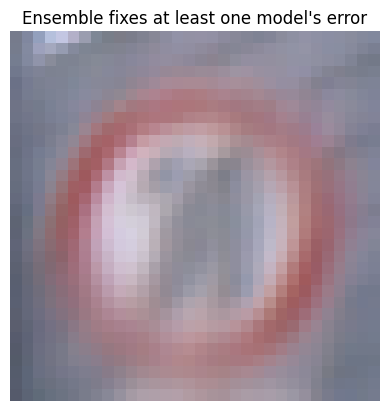
\includegraphics[width=0.9\linewidth]{images/hard_voting_fix.png}
    \caption{Example of an ensemble fix. Although a small number of models produce incorrect predictions, the majority vote correctly classifies the traffic sign.}
    \label{fig:hard_voting_fix}
\end{figure}

\begin{figure}[h]
    \centering
    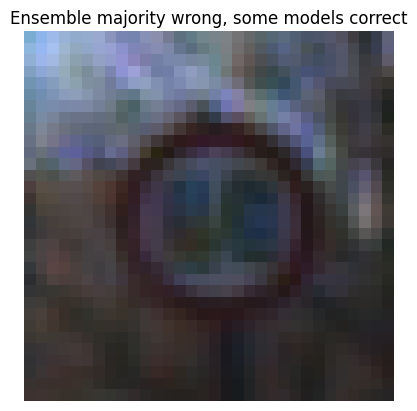
\includegraphics[width=0.9\linewidth]{images/hard_voting_amplify.png}
    \caption{Example of an ensemble amplification. The majority of models predict an incorrect class, causing the ensemble to misclassify a sample that some individual models classify correctly.}
    \label{fig:hard_voting_amplify}
\end{figure}






\subsection{Soft Voting Ensemble}

A soft voting ensemble was also evaluated using the same set of 33 trained models. Unlike hard voting, where only the predicted class of each model is considered, soft voting combines the confidence scores produced by all models. For each test sample, the class probabilities obtained after the softmax operation were averaged across all models, and the final prediction corresponded to the class with the highest aggregated probability.

The soft voting ensemble achieved a test accuracy of \textbf{99.60\%}, slightly outperforming the hard voting ensemble (\textbf{99.57\%}). This improvement suggests that incorporating prediction confidence provides additional information beyond the final class label, allowing the ensemble to make more reliable decisions in samples where model predictions are uncertain or partially conflicting.

Although the performance gain is relatively small, the results indicate that probability aggregation can exploit the complementary strengths of the augmentation-specialized models more effectively than simple majority voting. This leads to a modest but consistent improvement in classification performance, demonstrating the benefit of incorporating model confidence into the ensemble decision process.





\subsection{Weighted Soft Voting Ensemble}

A weighted soft voting ensemble was also evaluated to account for the fact that not all individual models achieved the same level of performance. Instead of assigning equal importance to every model, the contribution of each model was weighted according to its individual test accuracy. The weights were computed using a normalized exponential function, giving greater influence to the most accurate models while still preserving contributions from the remaining ensemble members.

The weighted probabilities produced by all models were then aggregated to obtain the final prediction for each test sample. Using this strategy, the ensemble achieved a test accuracy of \textbf{99.62\%}, representing the best result obtained across all evaluated models and ensemble configurations.

Compared to hard voting (\textbf{99.57\%}) and standard soft voting (\textbf{99.60\%}), the weighted soft voting ensemble provided a small but consistent improvement. This result suggests that emphasizing predictions from the strongest individual models while still leveraging the diversity introduced by different augmentation strategies yields the most effective overall classifier.















\section{Conclusion}

This work investigated the impact of multiple data augmentation strategies on traffic sign classification using the GTSRB dataset. Through a controlled experimental setup where all models shared the same architecture and training configuration, it was possible to isolate and analyze the contribution of each augmentation technique to model performance and generalization.

Figure~\ref{fig:final_comparison} summarizes the mean test accuracy obtained by all evaluated models, providing a global comparison between the baseline model, individual augmentation strategies, and combined augmentation approaches.

\begin{figure}[ht]
    \centering
    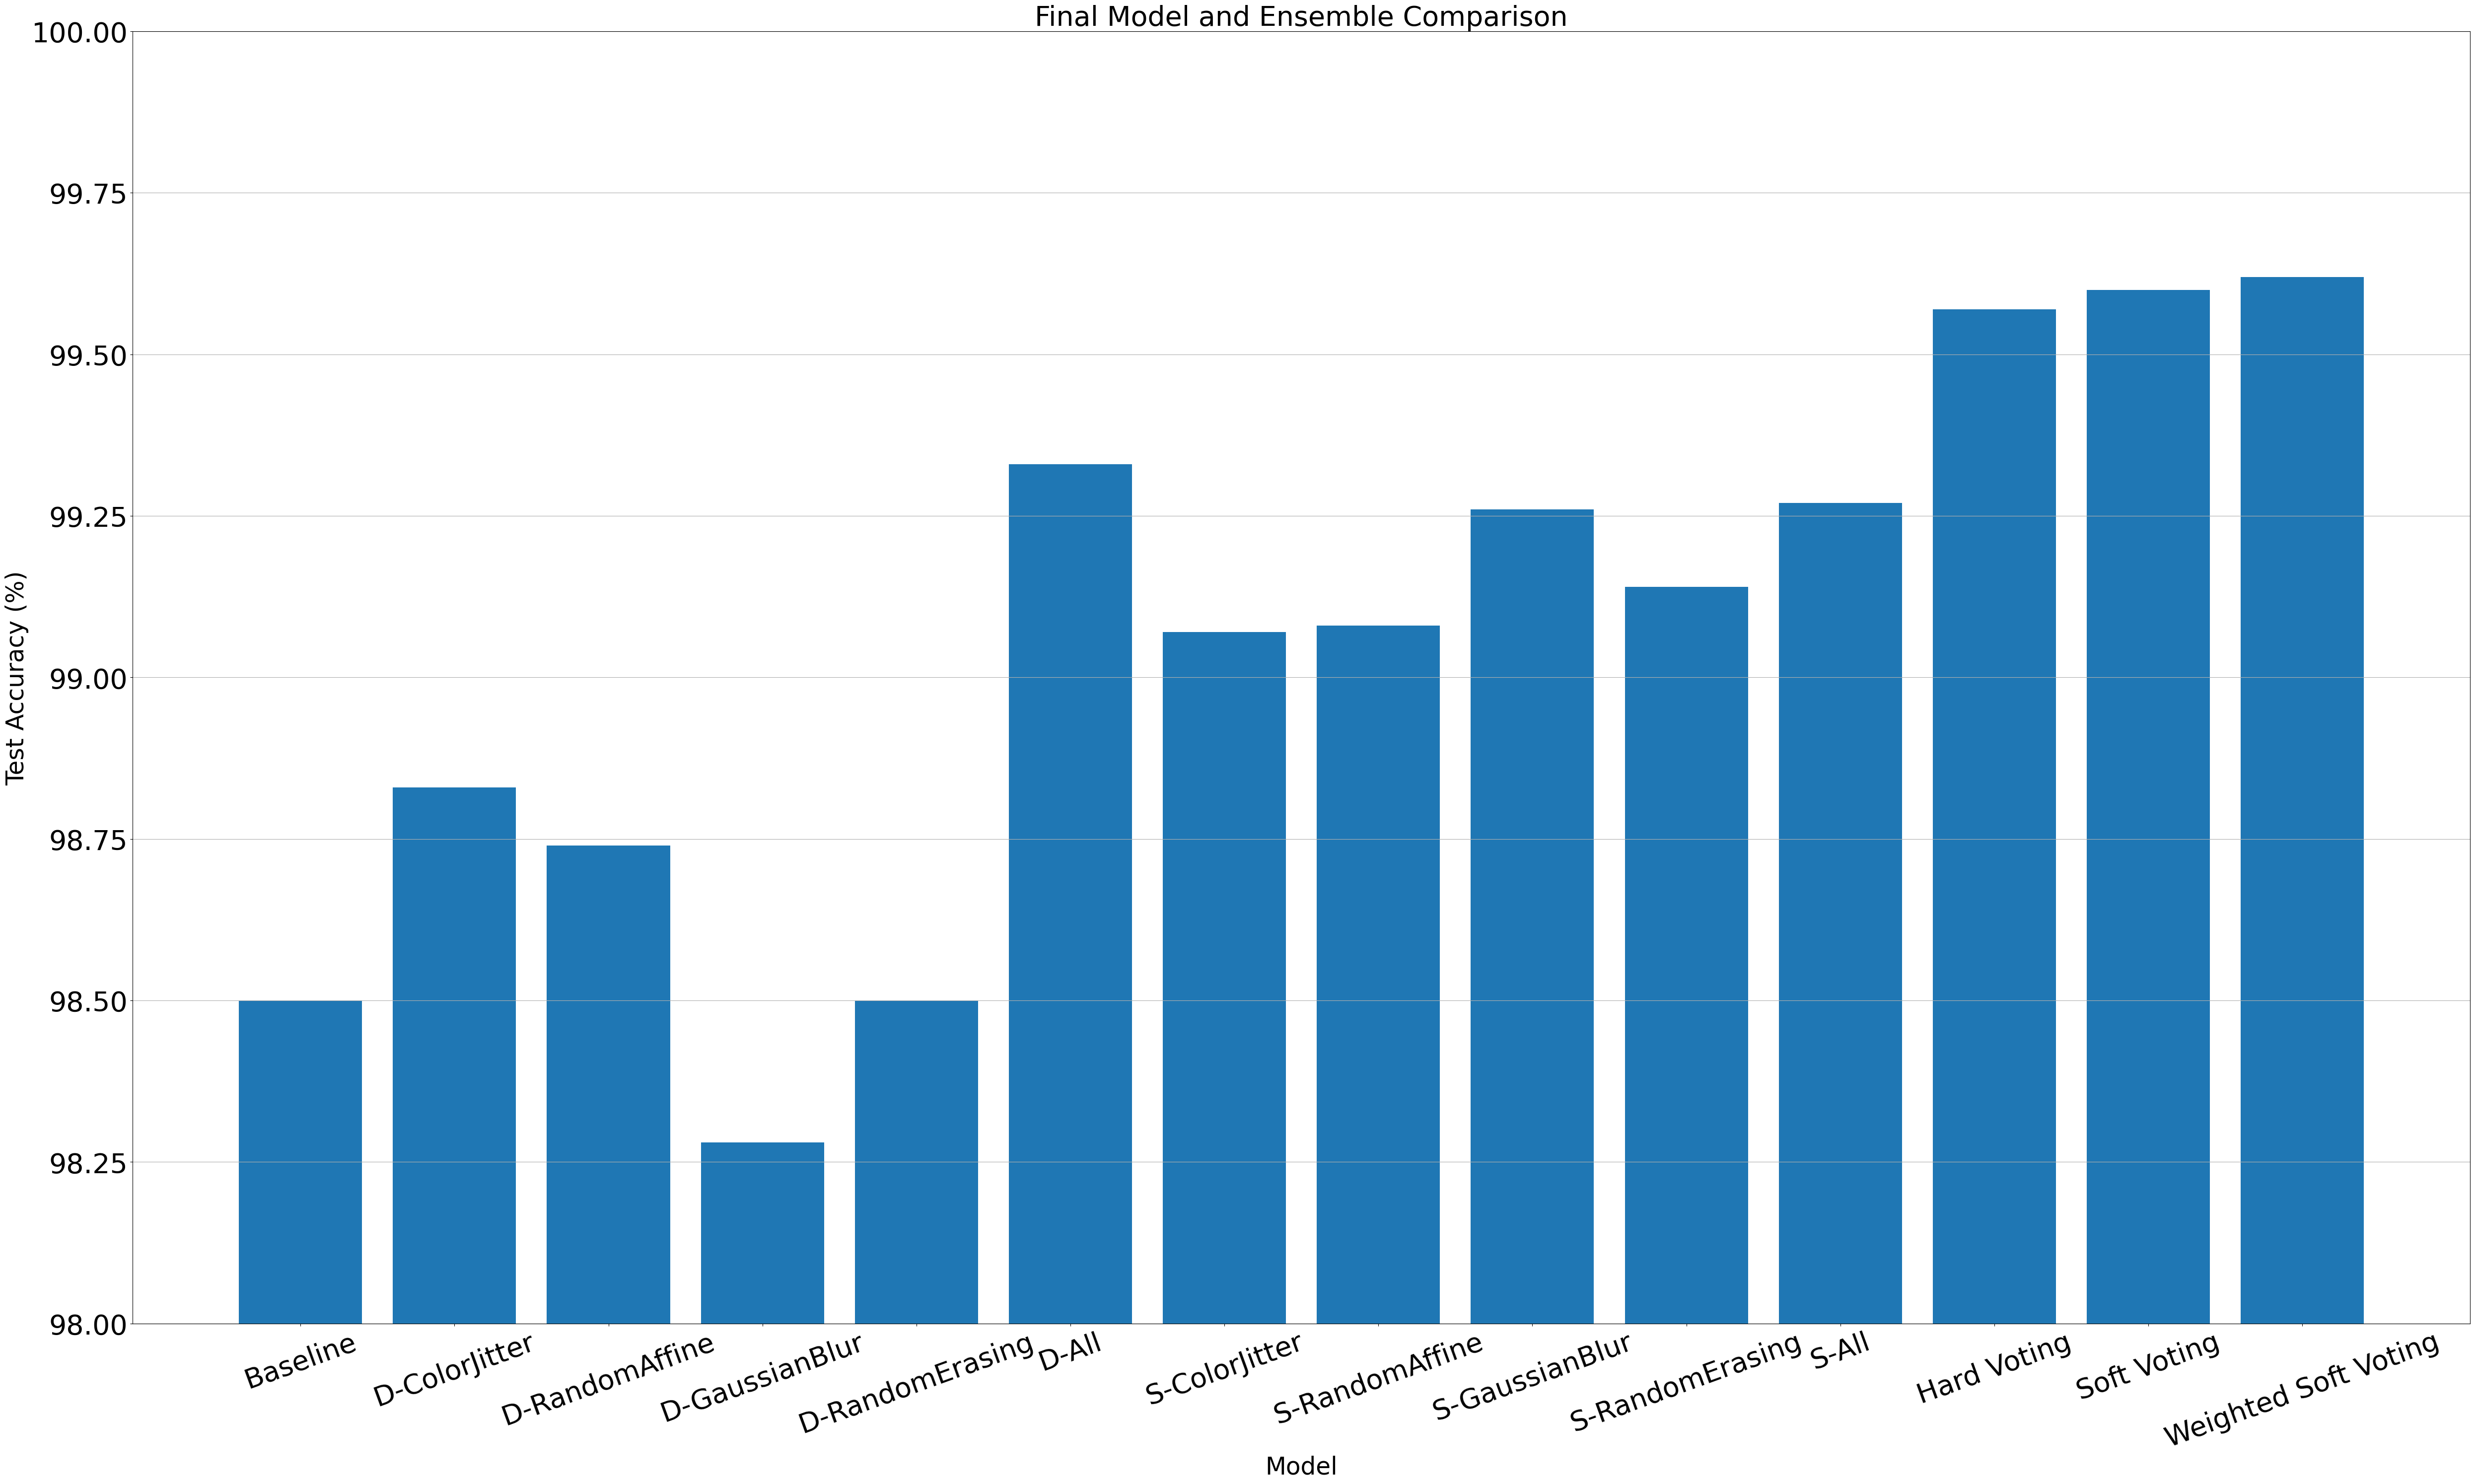
\includegraphics[width=1\linewidth]{images/final_comparision.png}
    \caption{Mean test accuracy comparison across all models.}
    \label{fig:final_comparison}
\end{figure}

The results demonstrate that data augmentation consistently improves classification performance when compared to the baseline model. While individual augmentation techniques provided gains by addressing specific failure modes, the strongest results were obtained through combined augmentation pipelines, which exposed the network to a broader range of visual variations during training.

Among the individual models, the Dynamic Combined Augmentation achieved the highest accuracy (\textbf{99.33\%}), closely followed by the Static Combined Augmentation (\textbf{99.27\%}) and Static Gaussian Blur (\textbf{99.26\%}). The qualitative analysis of confusion matrices and misclassified samples further revealed that different augmentation strategies tend to specialize in different types of challenging samples, confirming that their strengths are largely complementary.

Motivated by this observation, several ensemble methods were evaluated using all trained models. The results showed that combining models trained under different augmentation regimes provides additional gains beyond those achievable by any individual model. Hard voting reached \textbf{99.57\%} accuracy, while soft voting slightly improved the result to \textbf{99.60\%}. The best overall performance was obtained with the Weighted Soft Voting Ensemble, achieving \textbf{99.62\%} test accuracy. This represents the highest accuracy observed throughout the study and confirms that weighting model contributions according to their individual performance allows the ensemble to exploit both model diversity and prediction reliability.

Overall, the experiments show that augmentation diversity is a key factor for improving robustness and generalization in traffic sign recognition tasks. Furthermore, the ensemble analysis demonstrates that models trained with different augmentation strategies learn complementary decision boundaries, enabling the correction of many individual model errors when their predictions are combined.

Future work could focus on evaluating additional augmentation techniques and testing the proposed approaches on other traffic sign datasets to verify their generalization capabilities. It would also be interesting to investigate whether similar improvements can be obtained using more recent deep learning architectures and smaller ensembles with fewer models but comparable performance.




\appendix

\section{Additional Visual Results}

Due to space and layout constraints in the main text, all confusion matrices and misclassification visualizations for the evaluated models are provided in this appendix. These figures complement the quantitative results presented in the main body of the report and allow a more detailed qualitative inspection of model behaviour across different augmentation strategies.

The following sections include the full set of visual results for both dynamic and static augmentation experiments, including confusion matrices and examples of incorrectly classified samples for each model configuration.

\subsection{Baseline Model}

\begin{figure}[h]
    \centering
    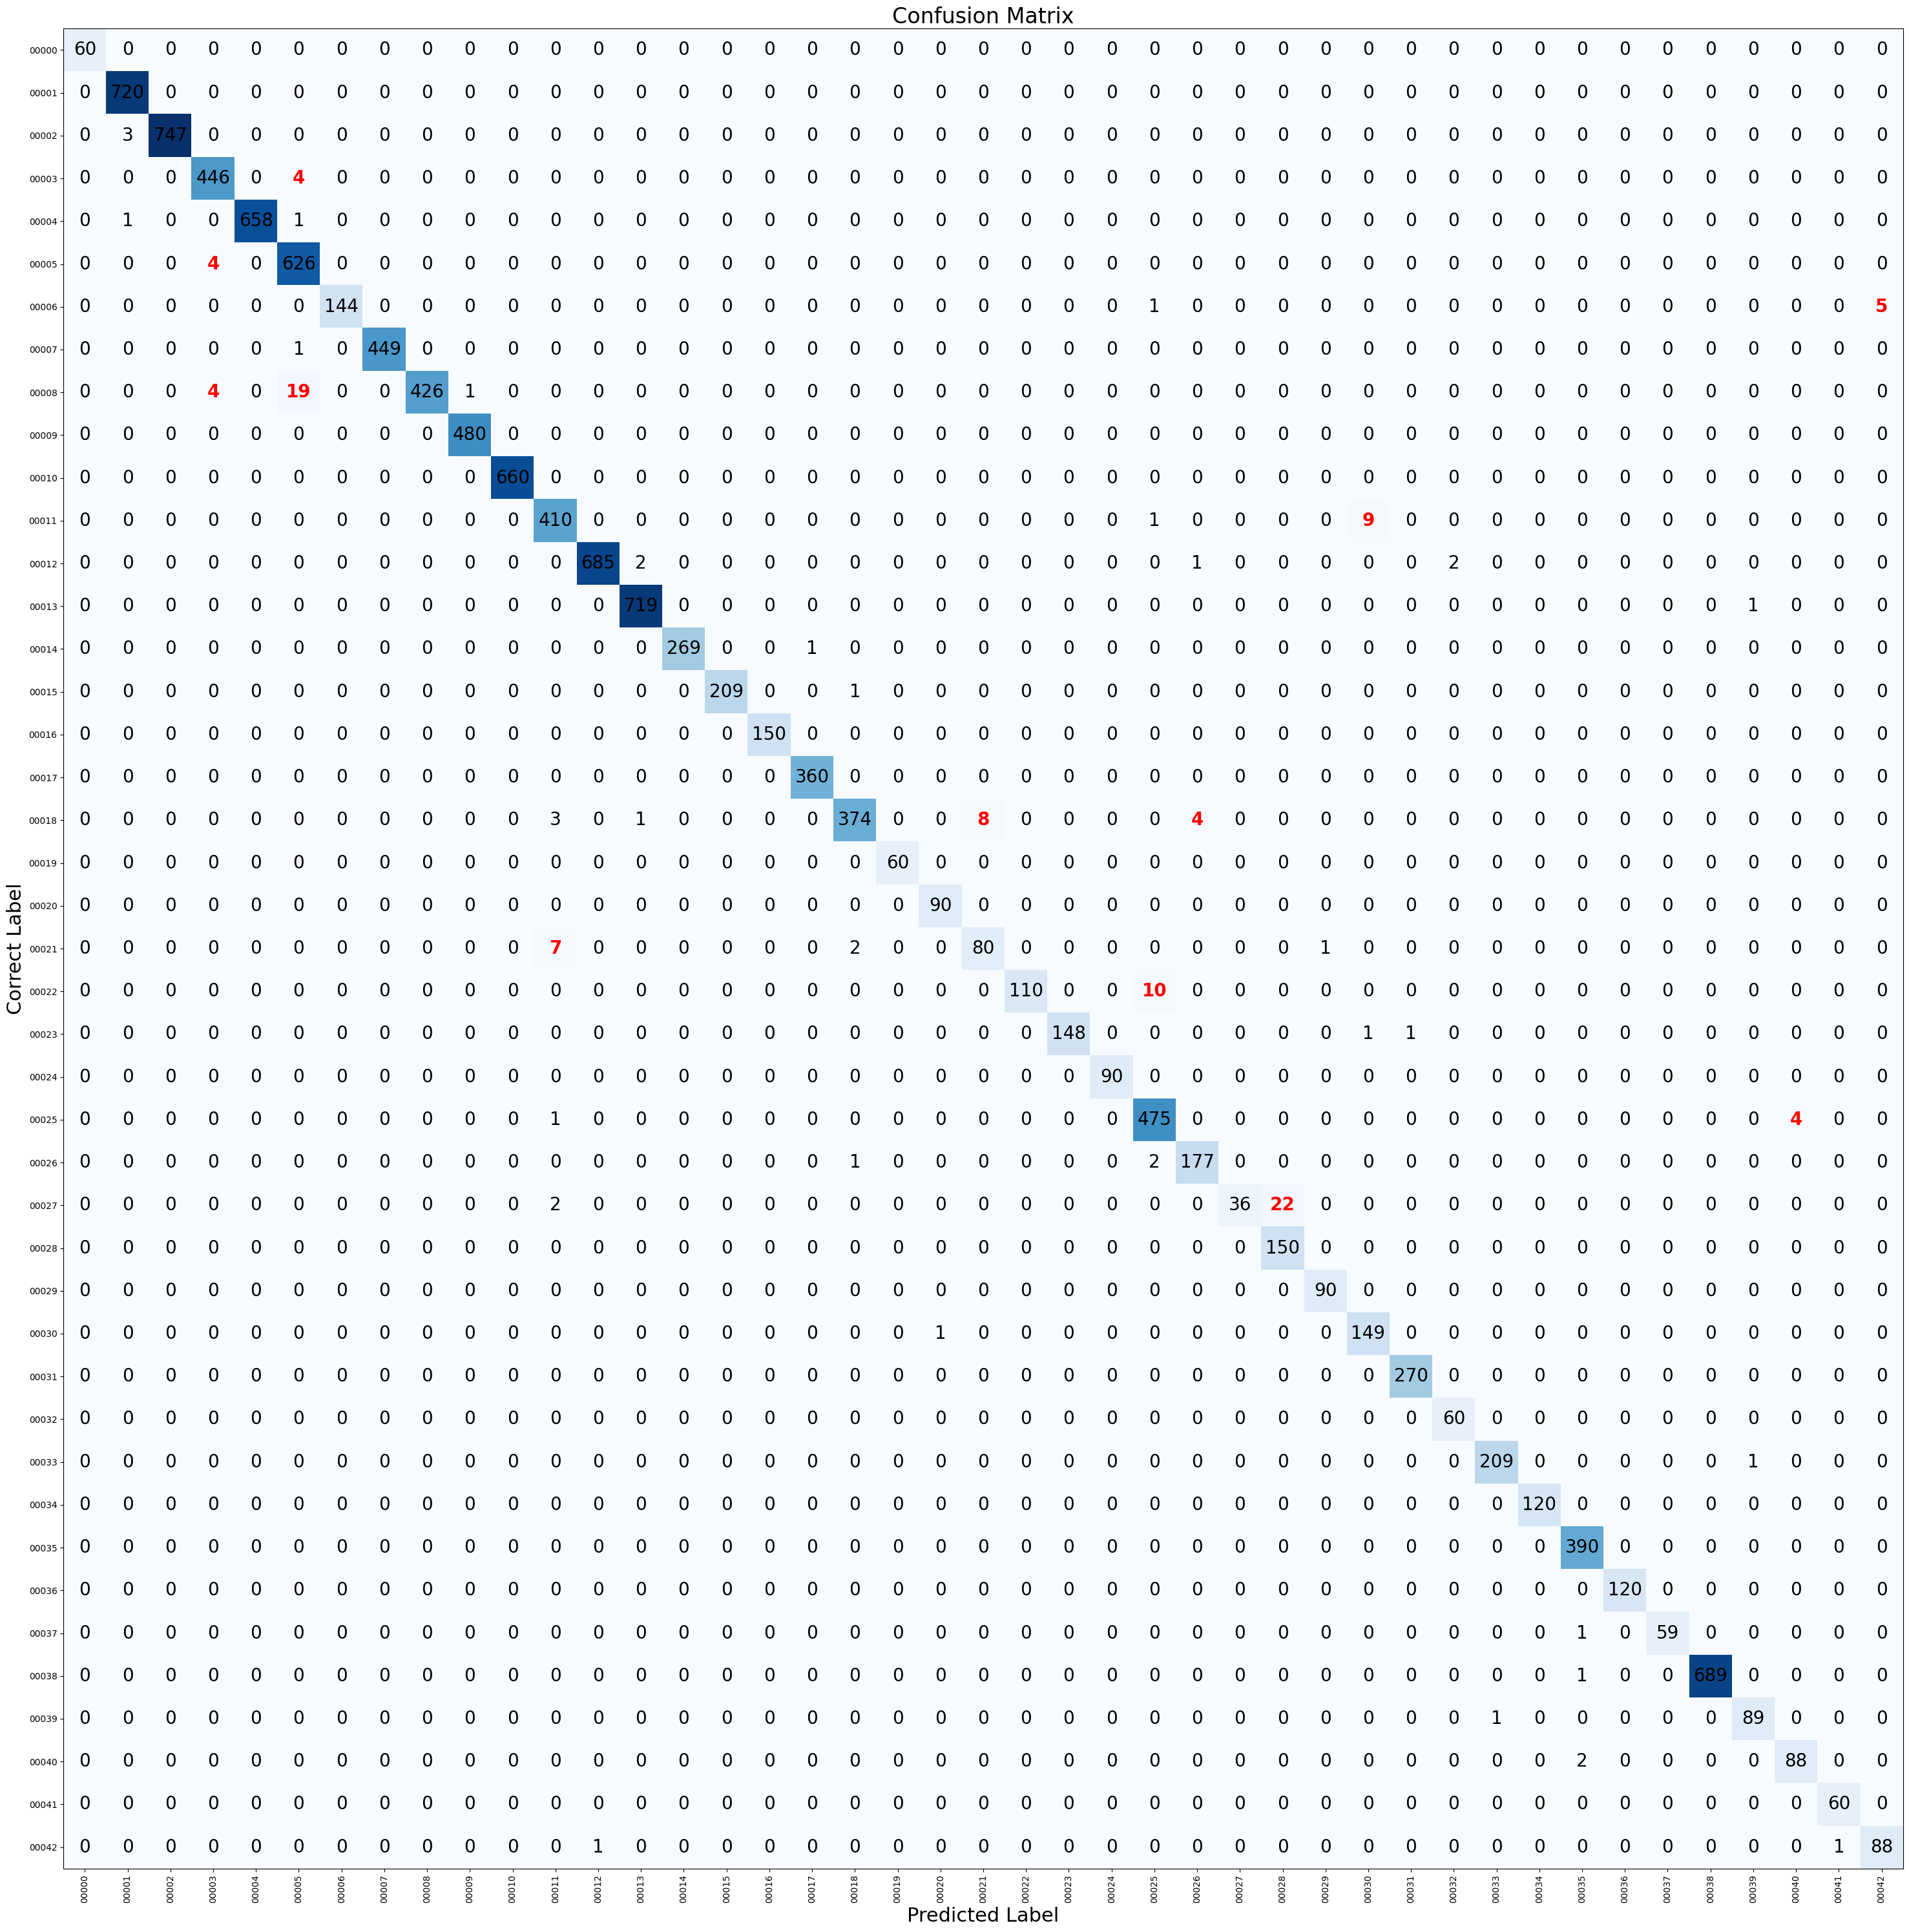
\includegraphics[width=0.8\linewidth]{images/baseline_confusion_matrix.png}
    \caption{Baseline model confusion matrix.}
    \label{fig:baseline_confusion_matrix}
\end{figure}

\begin{figure}[h]
    \centering
    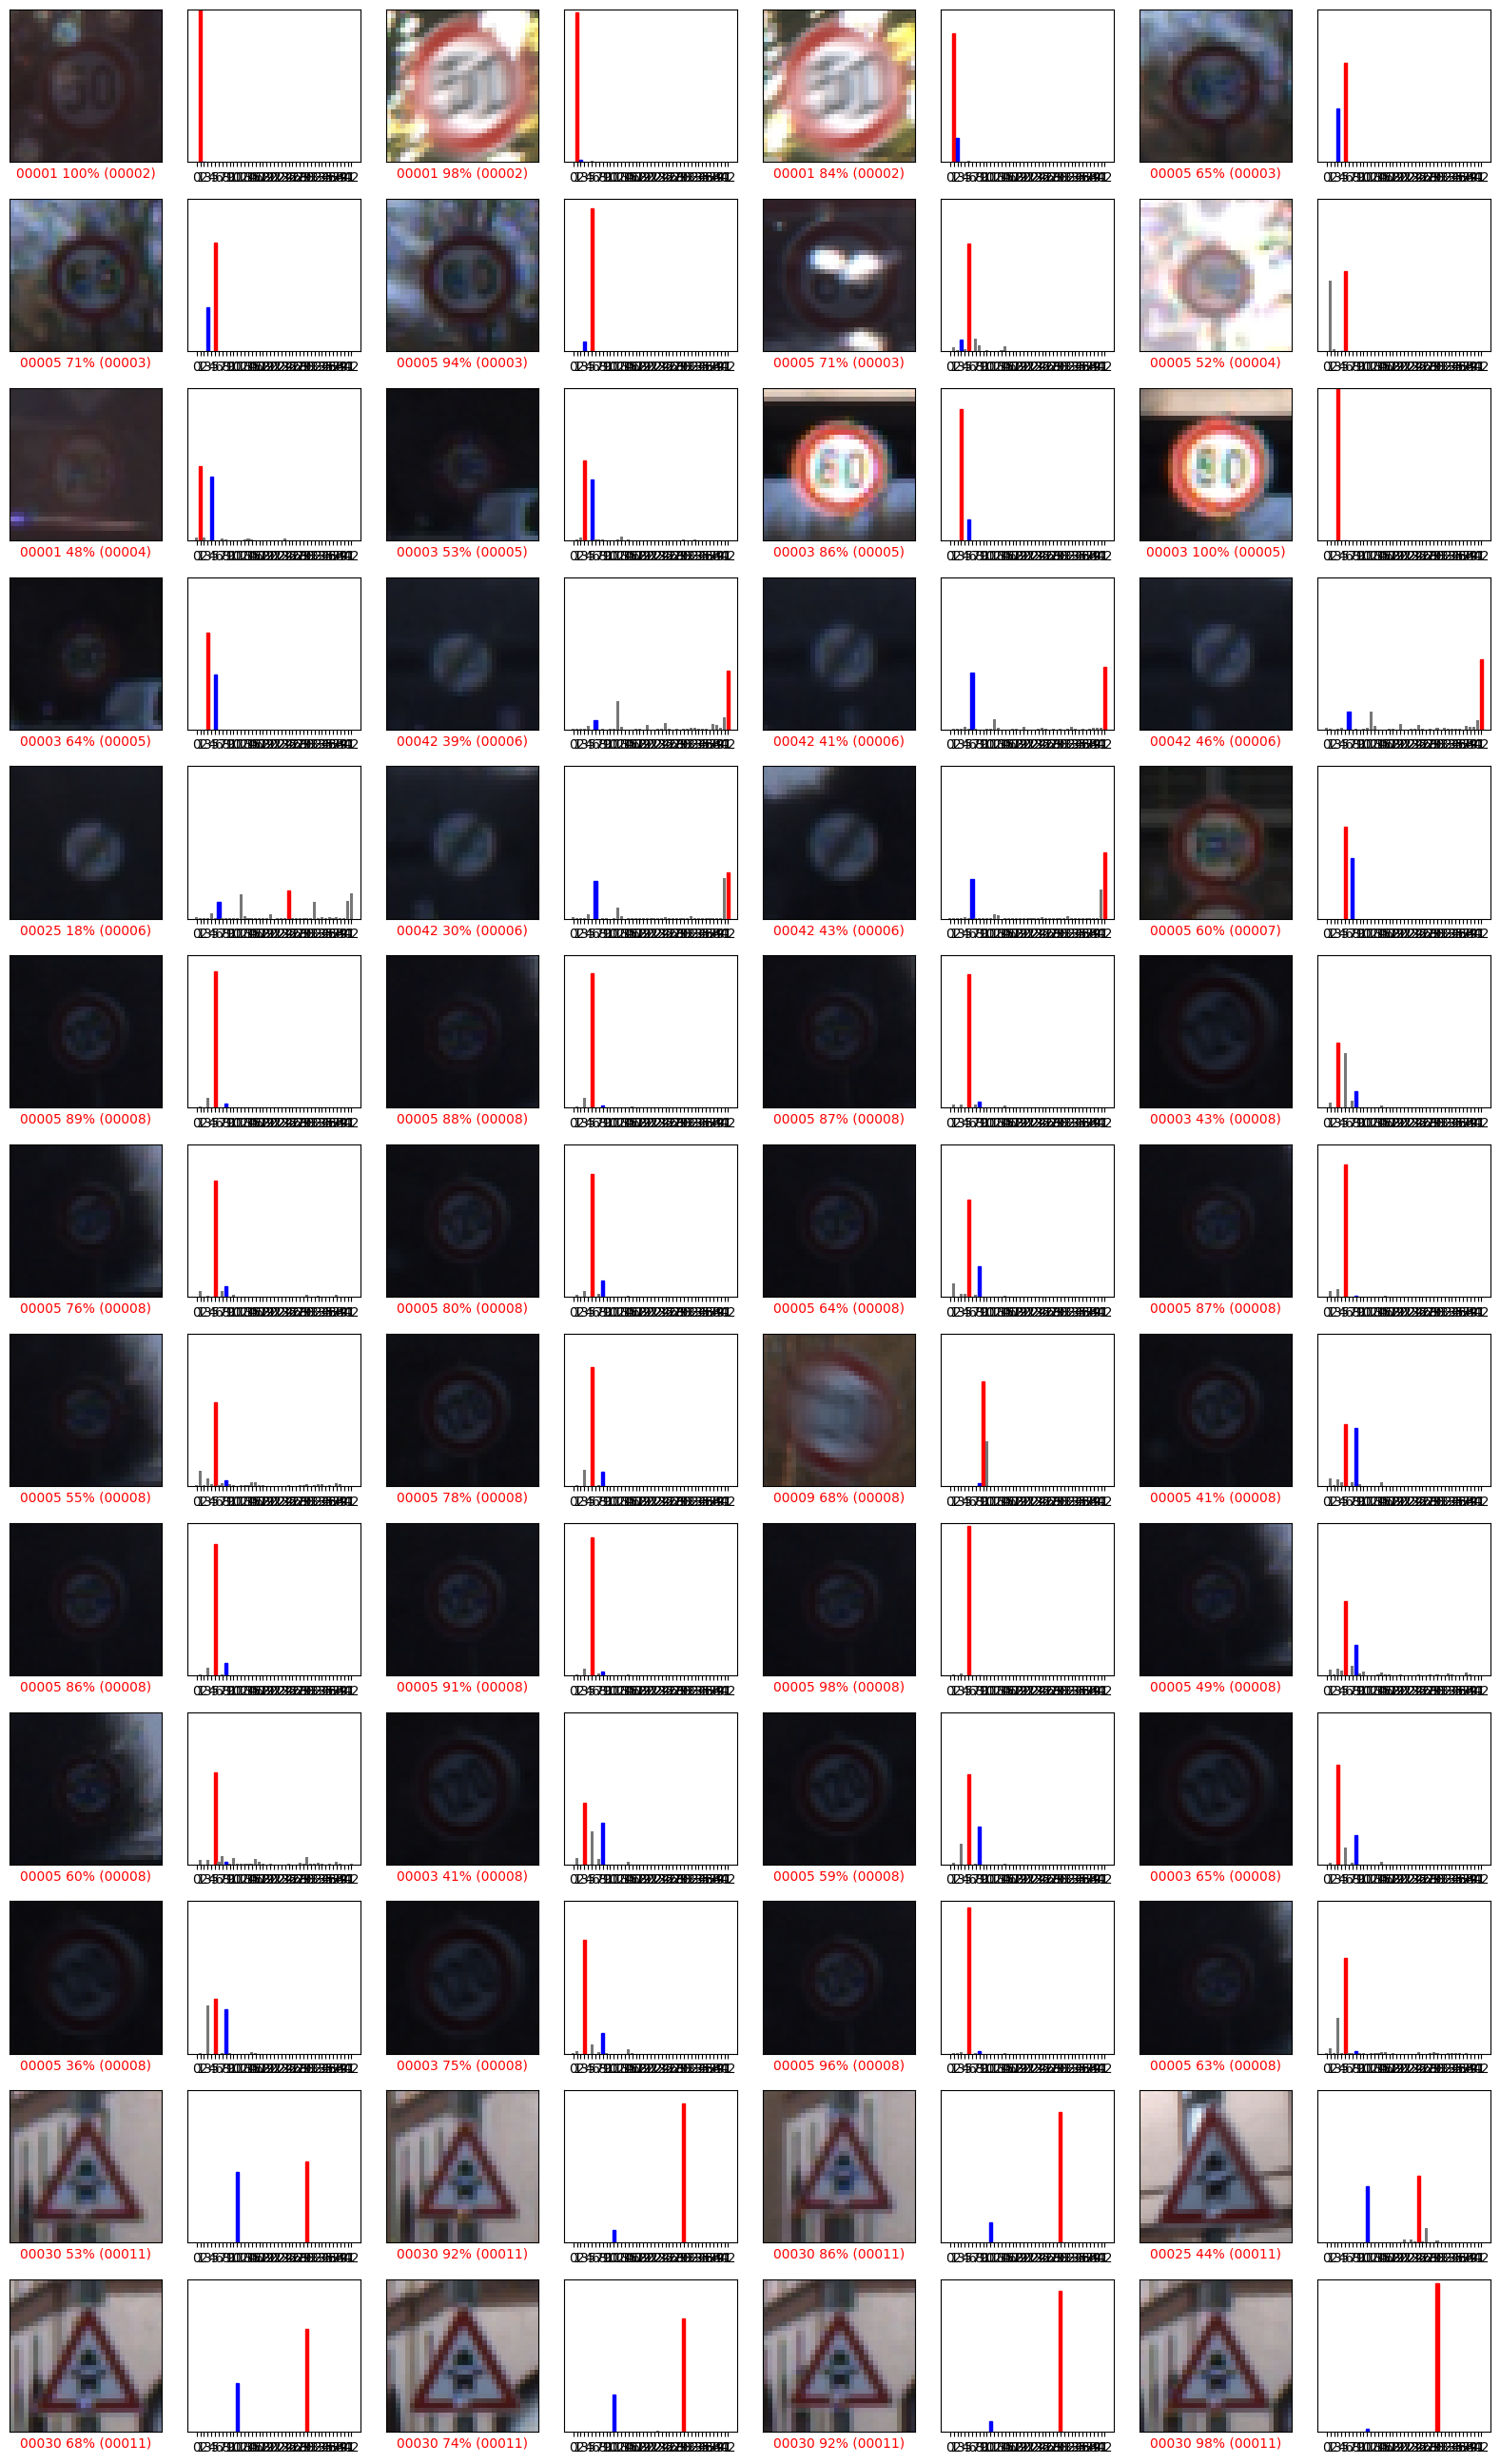
\includegraphics[width=0.8\linewidth]{images/baseline_bad_predictions.png}
    \caption{Baseline model misclassified samples.}
    \label{fig:baseline_bad_predictions}
\end{figure}

\subsection{Dynamic Models}

\subsubsection{ColorJitter}

\begin{figure}[h]
    \centering
    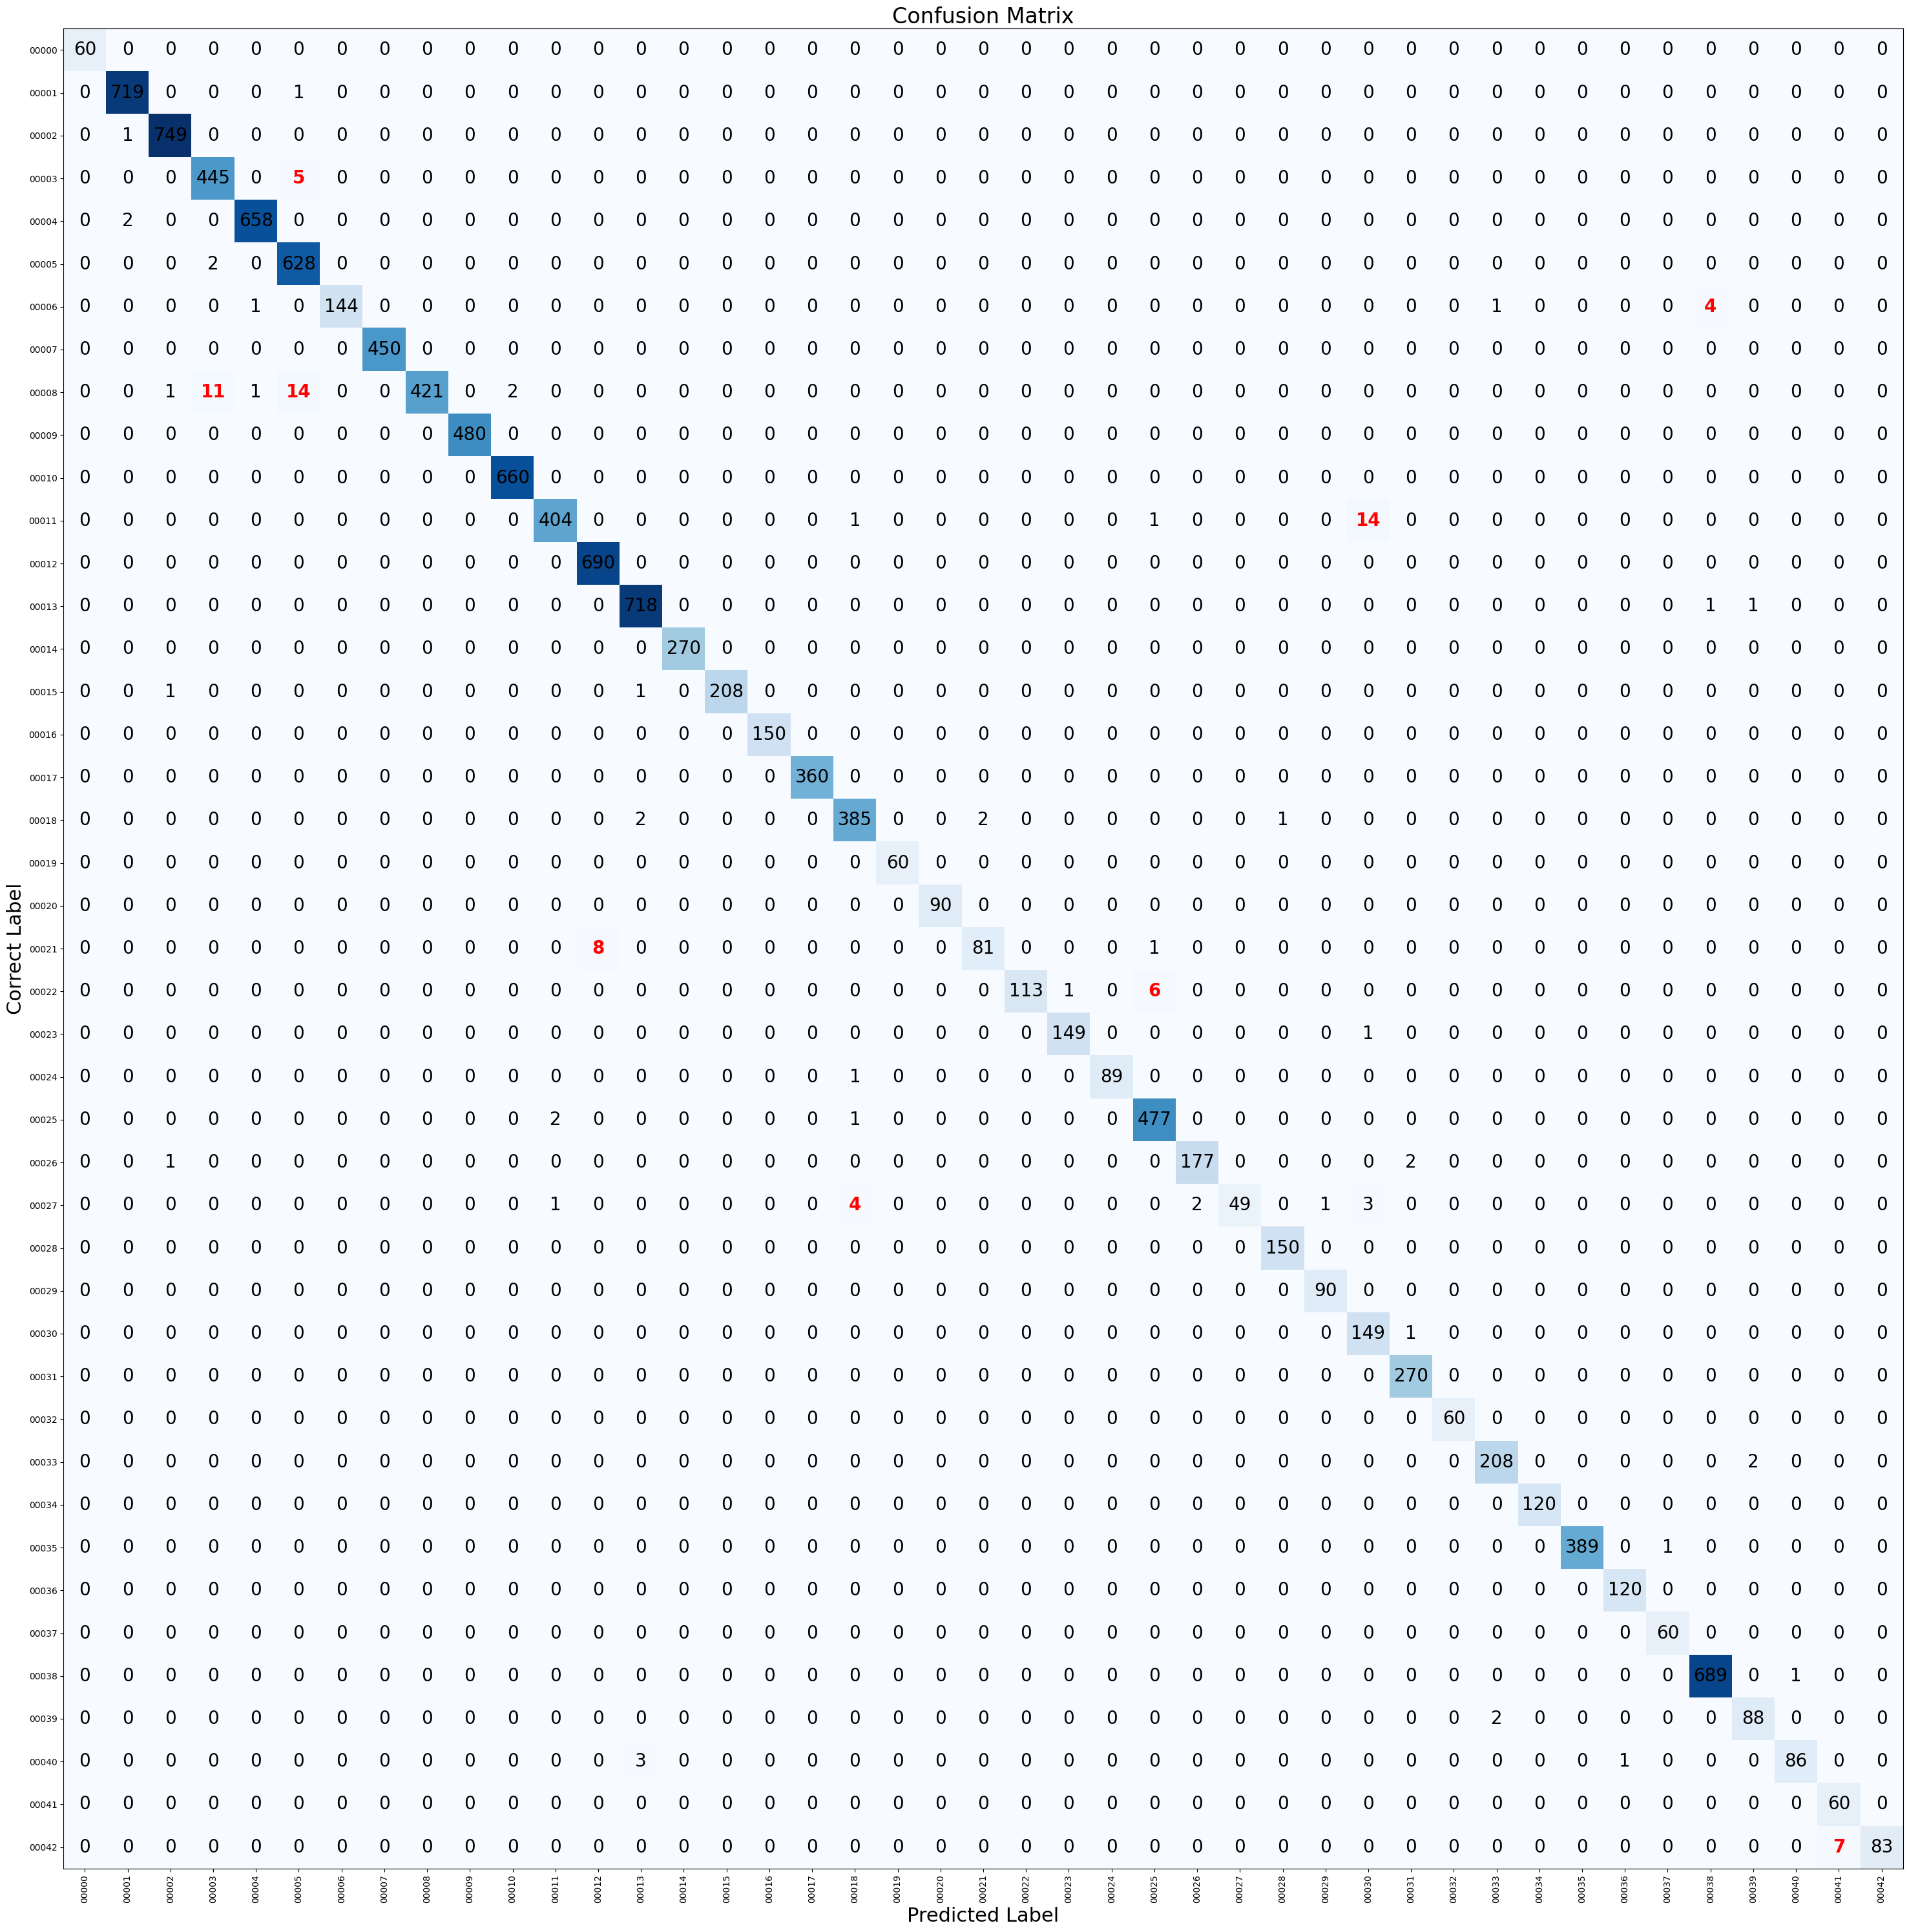
\includegraphics[width=0.8\linewidth]{images/colorjitter_confusion_matrix.png}
    \caption{Dynamic ColorJitter confusion matrix.}
    \label{fig:colorjitter_confusion_matrix}
\end{figure}

\begin{figure}[h]
    \centering
    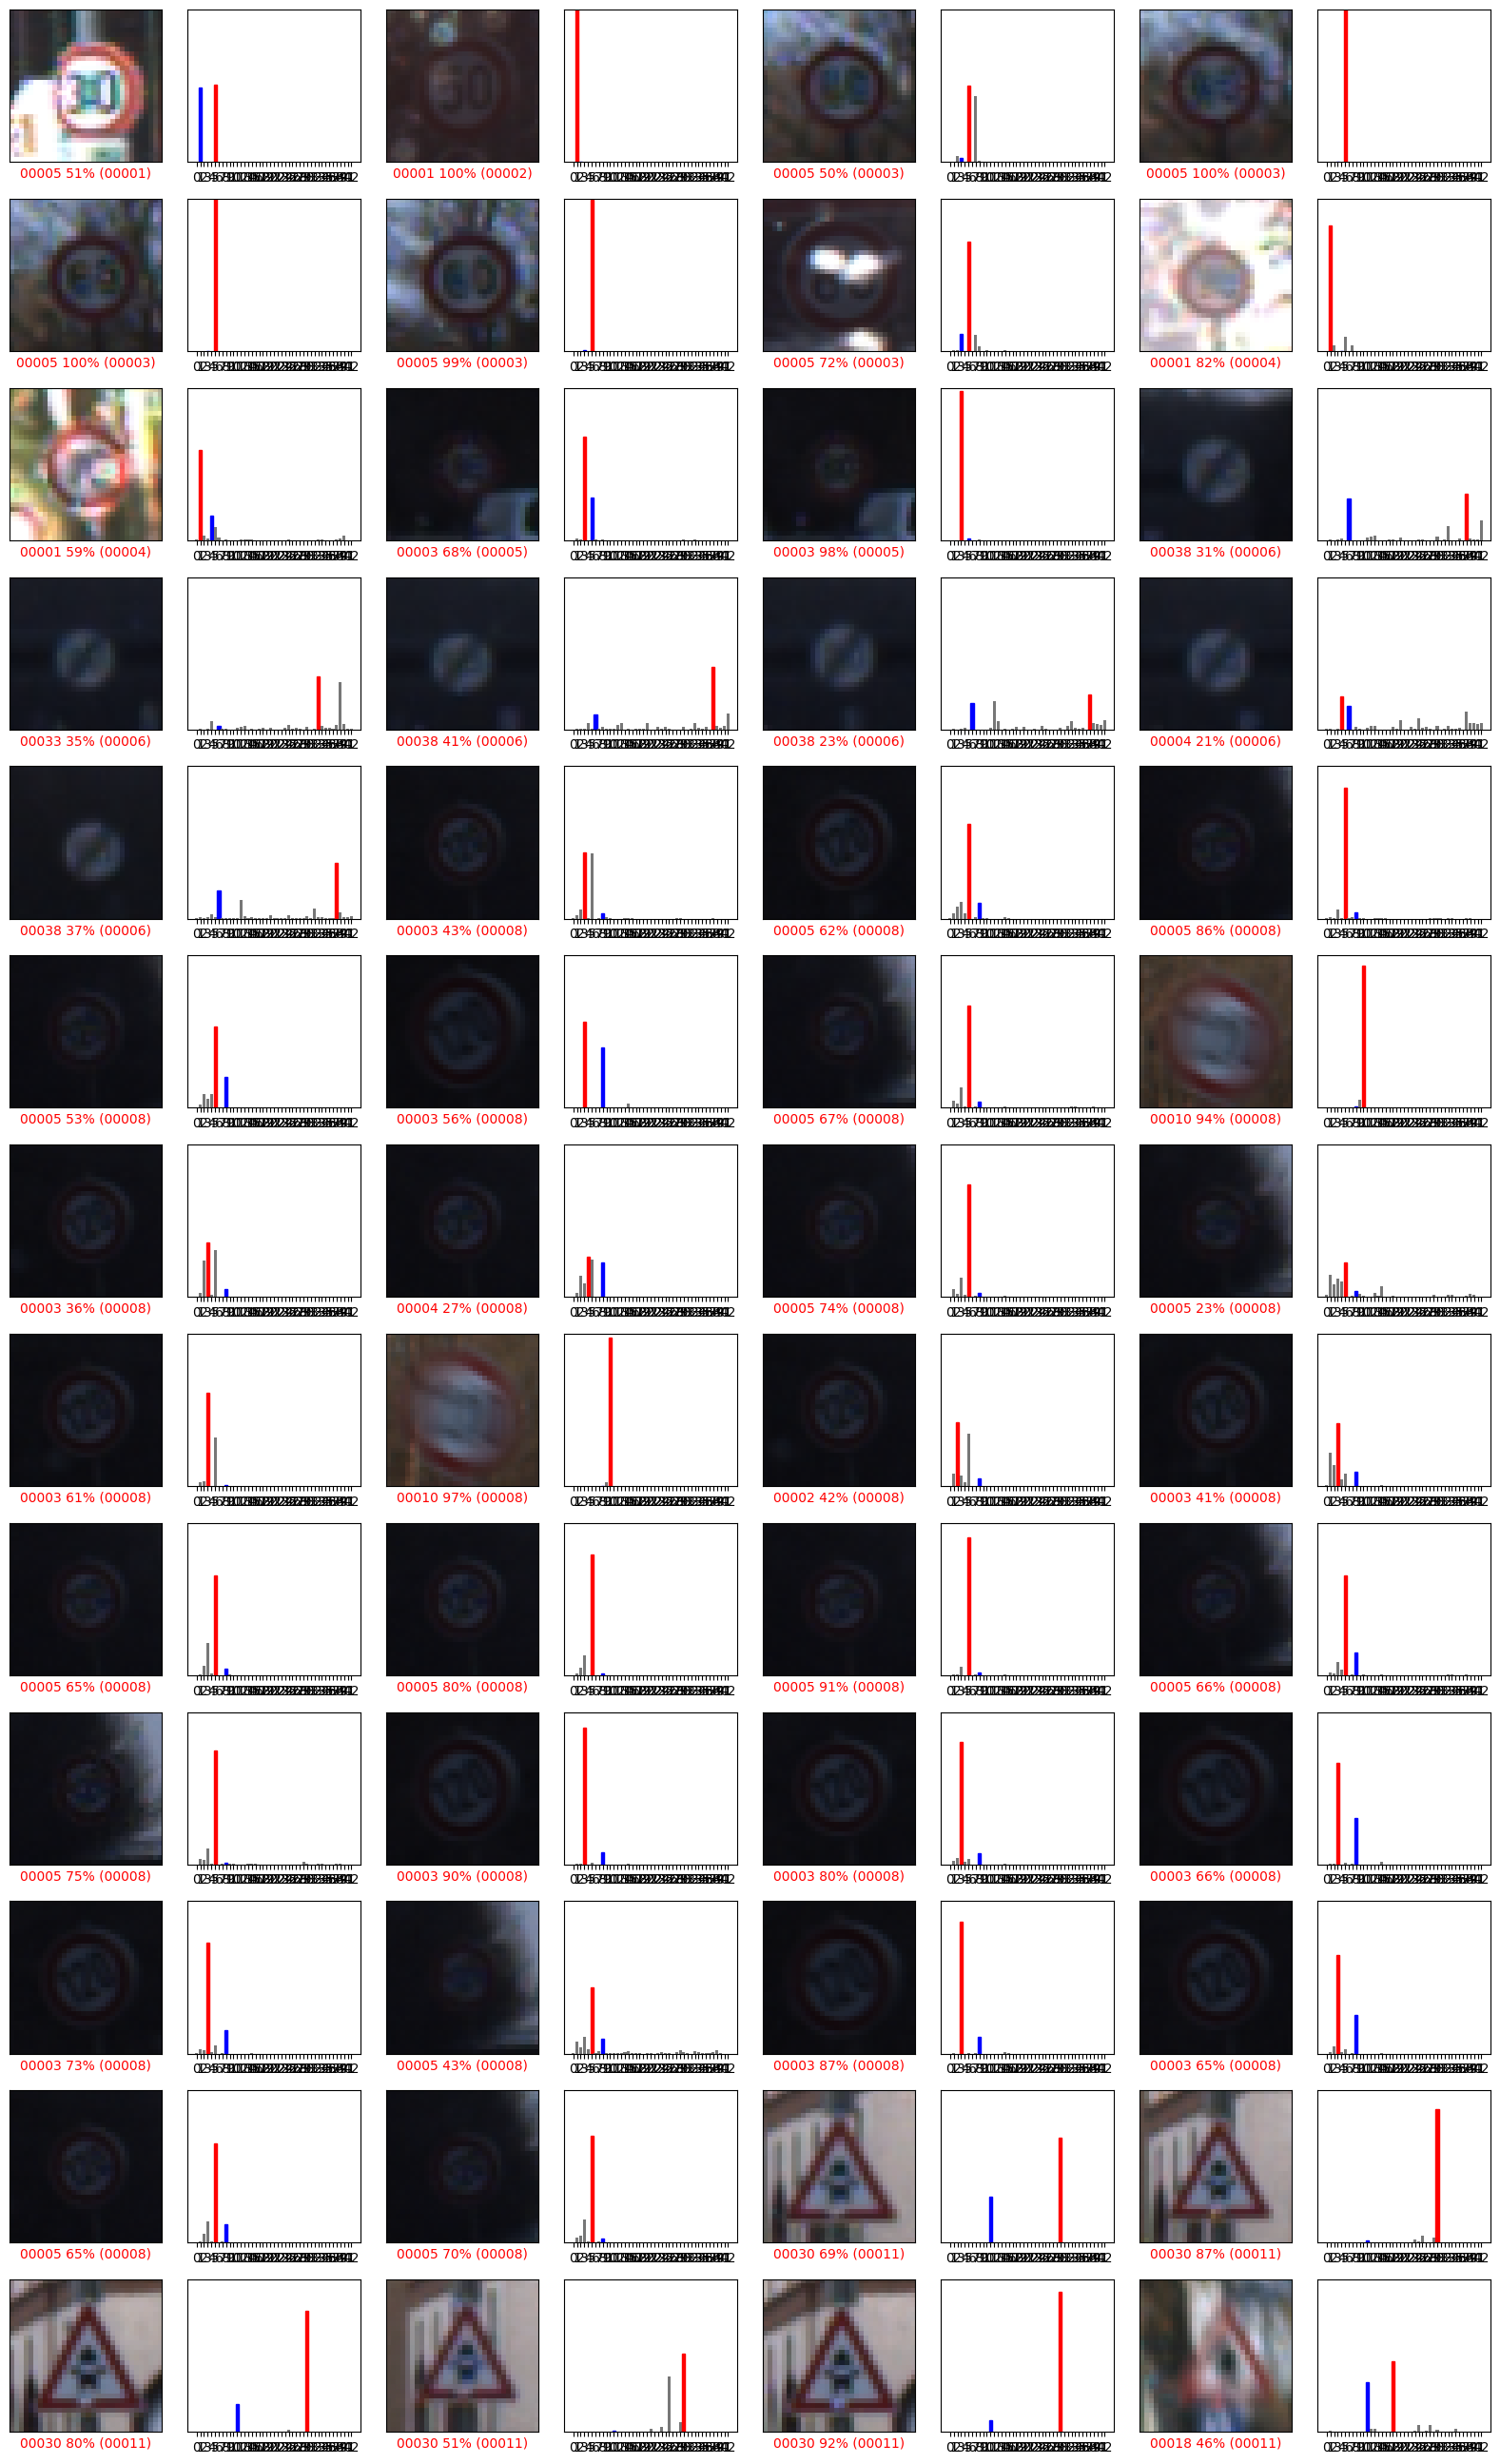
\includegraphics[width=0.8\linewidth]{images/colorjitter_bad_predictions.png}
    \caption{Dynamic ColorJitter misclassified samples.}
    \label{fig:colorjitter_bad_predictions}
\end{figure}

\subsubsection{RandomAffine}

\begin{figure}[h]
    \centering
    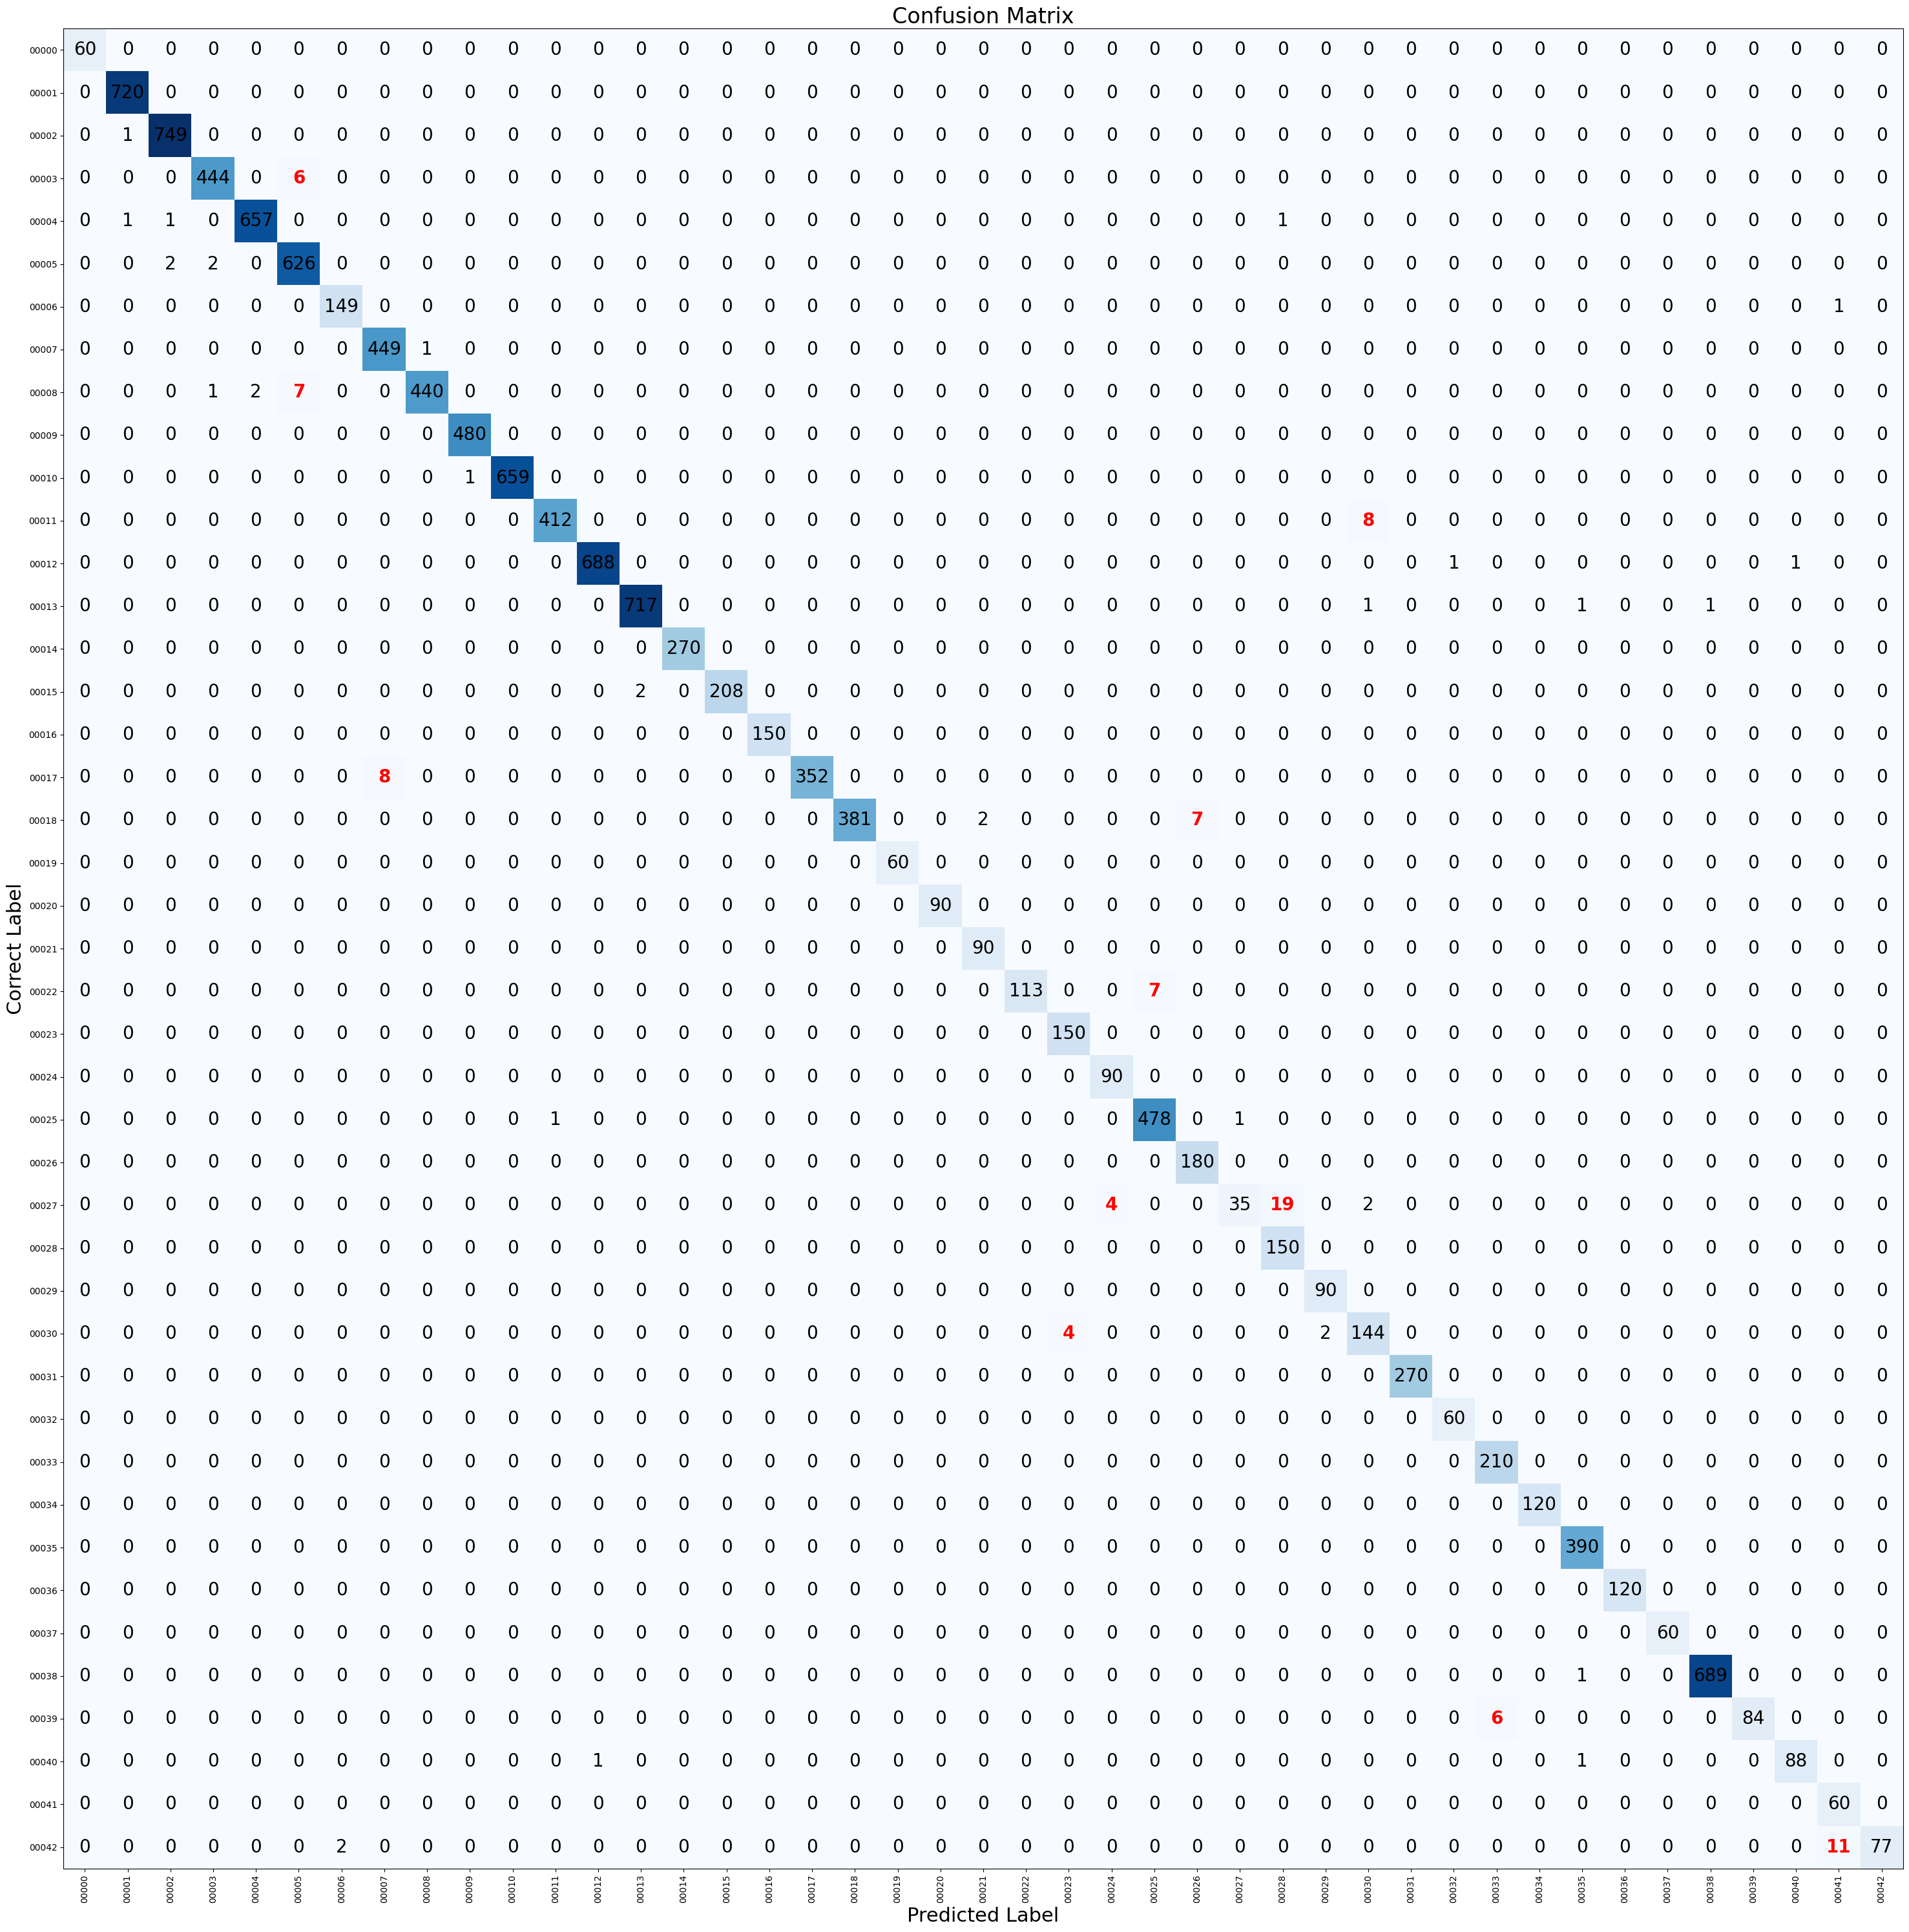
\includegraphics[width=0.8\linewidth]{images/affine_confusion_matrix.png}
    \caption{Dynamic RandomAffine confusion matrix.}
    \label{fig:affine_confusion_matrix}
\end{figure}

\begin{figure}[h]
    \centering
    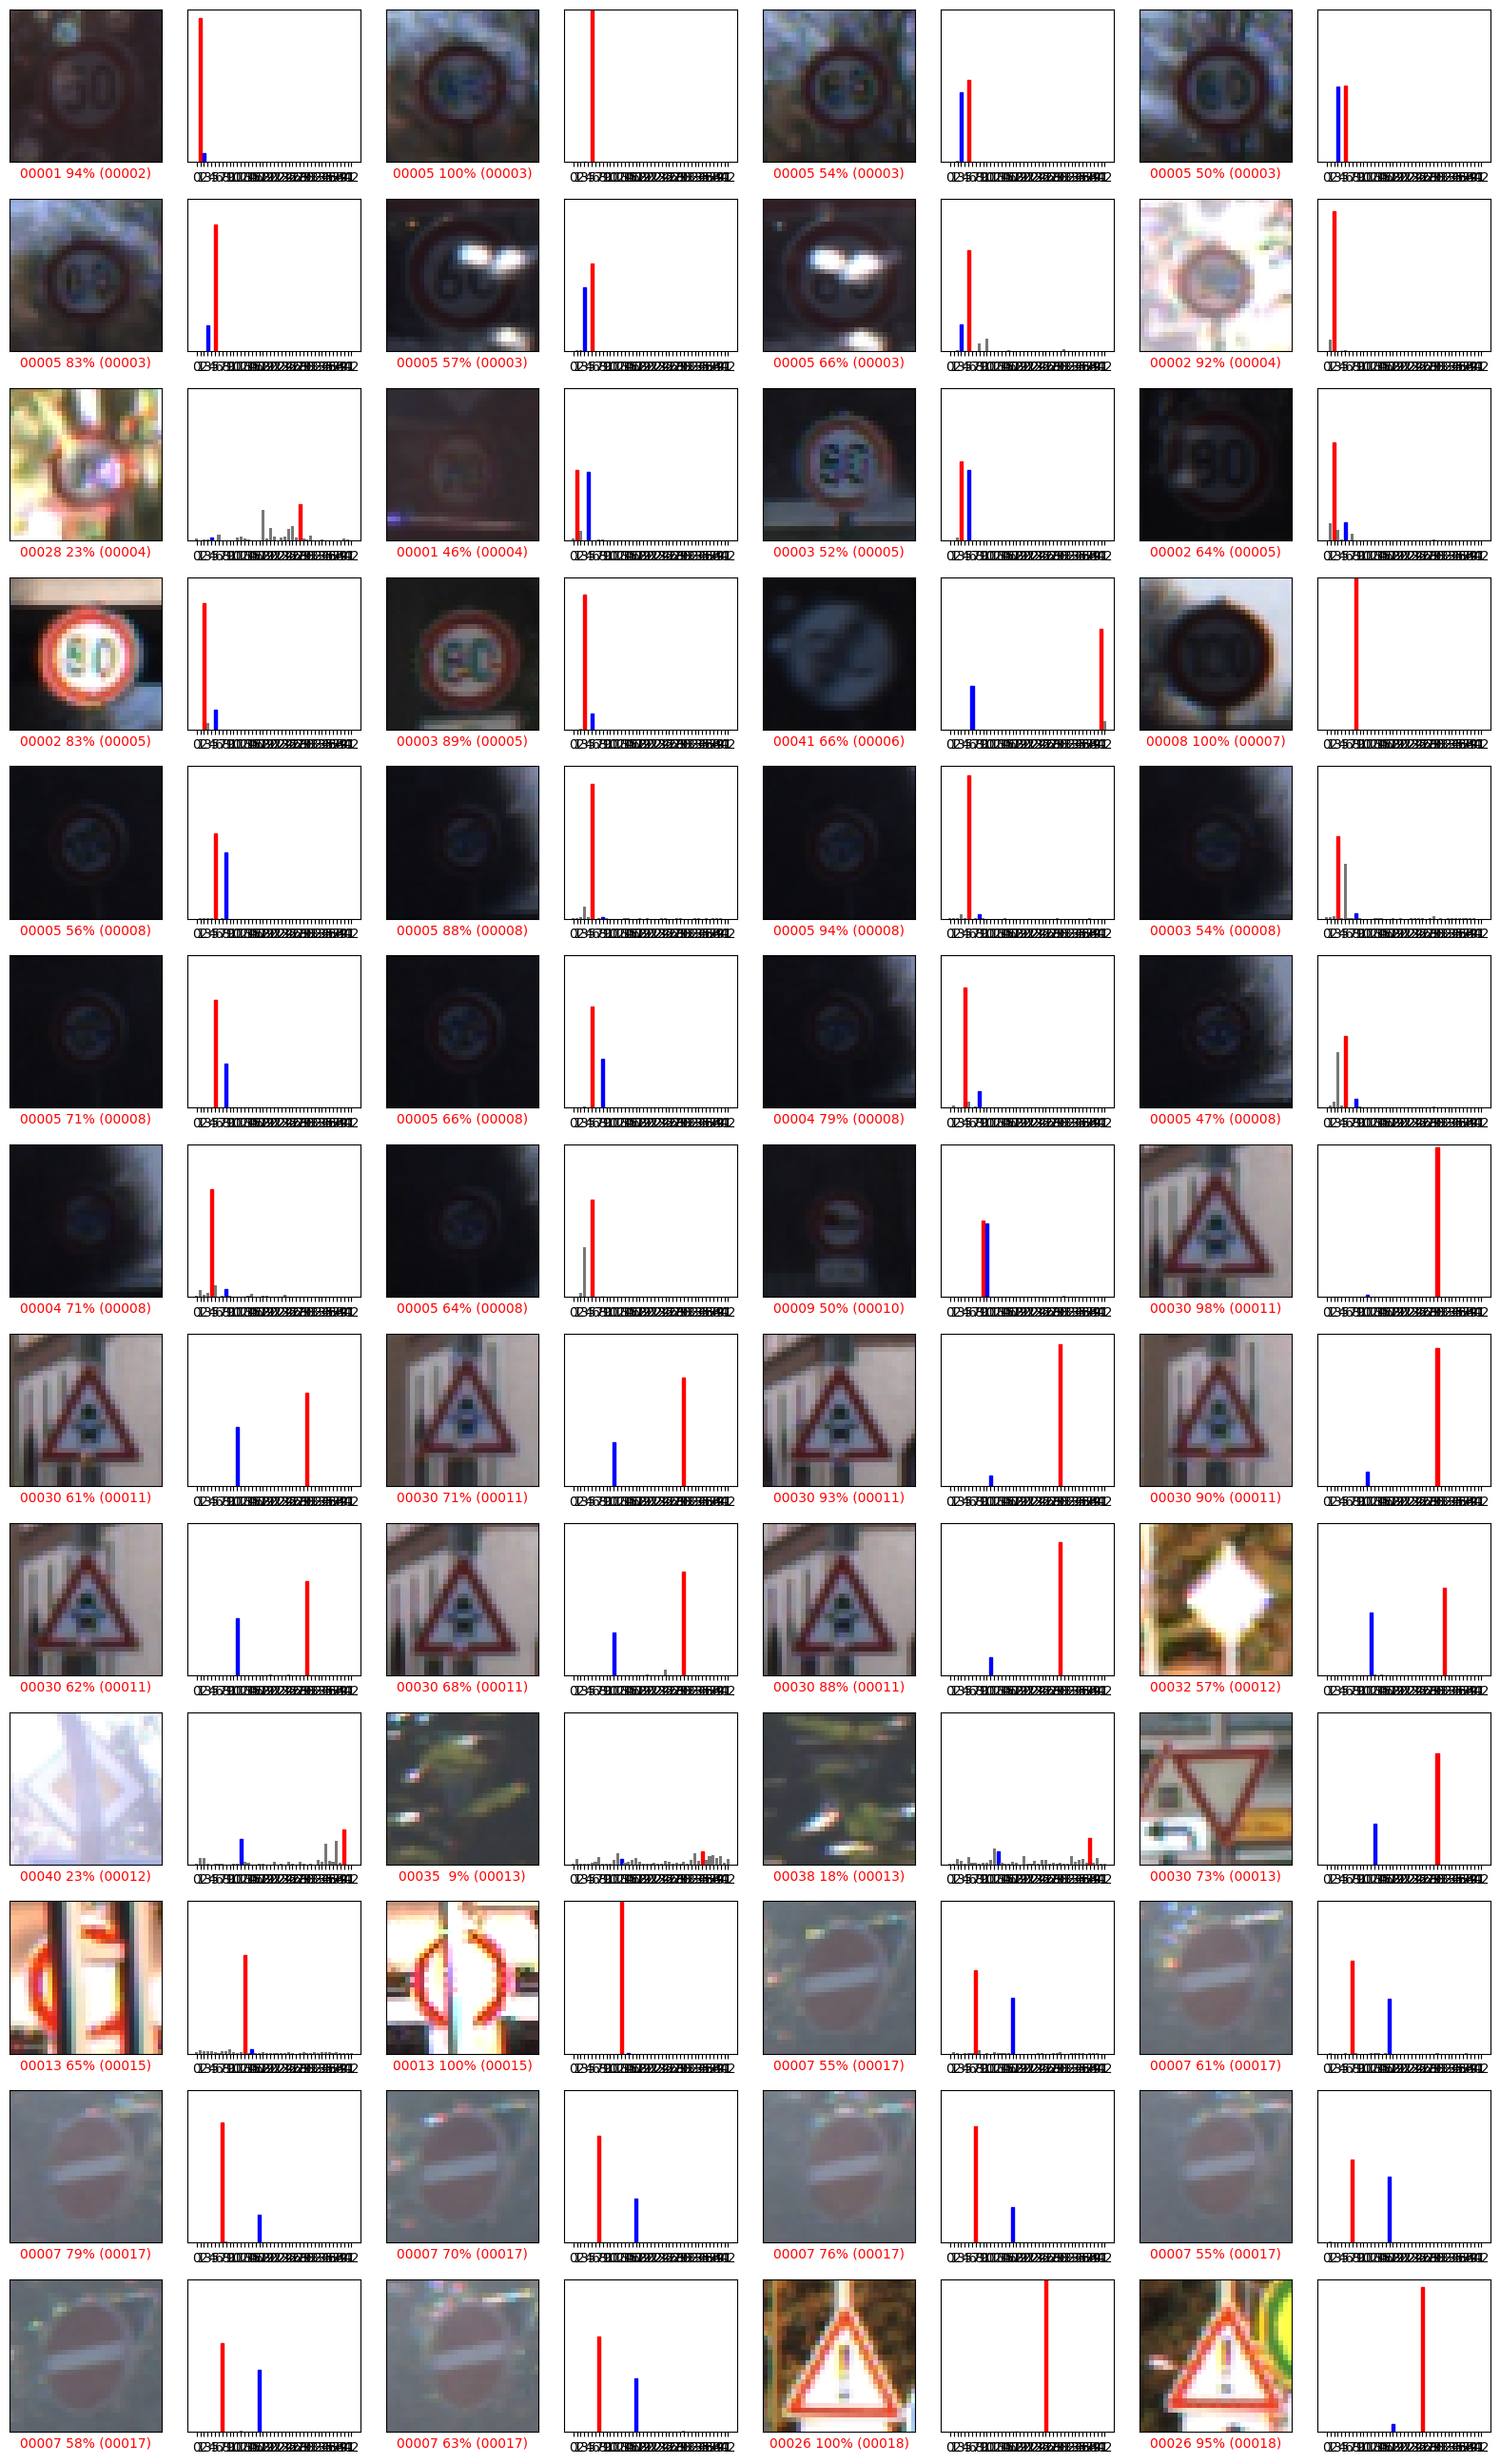
\includegraphics[width=0.8\linewidth]{images/affine_bad_predictions.png}
    \caption{Dynamic RandomAffine misclassified samples.}
    \label{fig:affine_bad_predictions}
\end{figure}

\subsubsection{Gaussian Blur}

\begin{figure}[h]
    \centering
    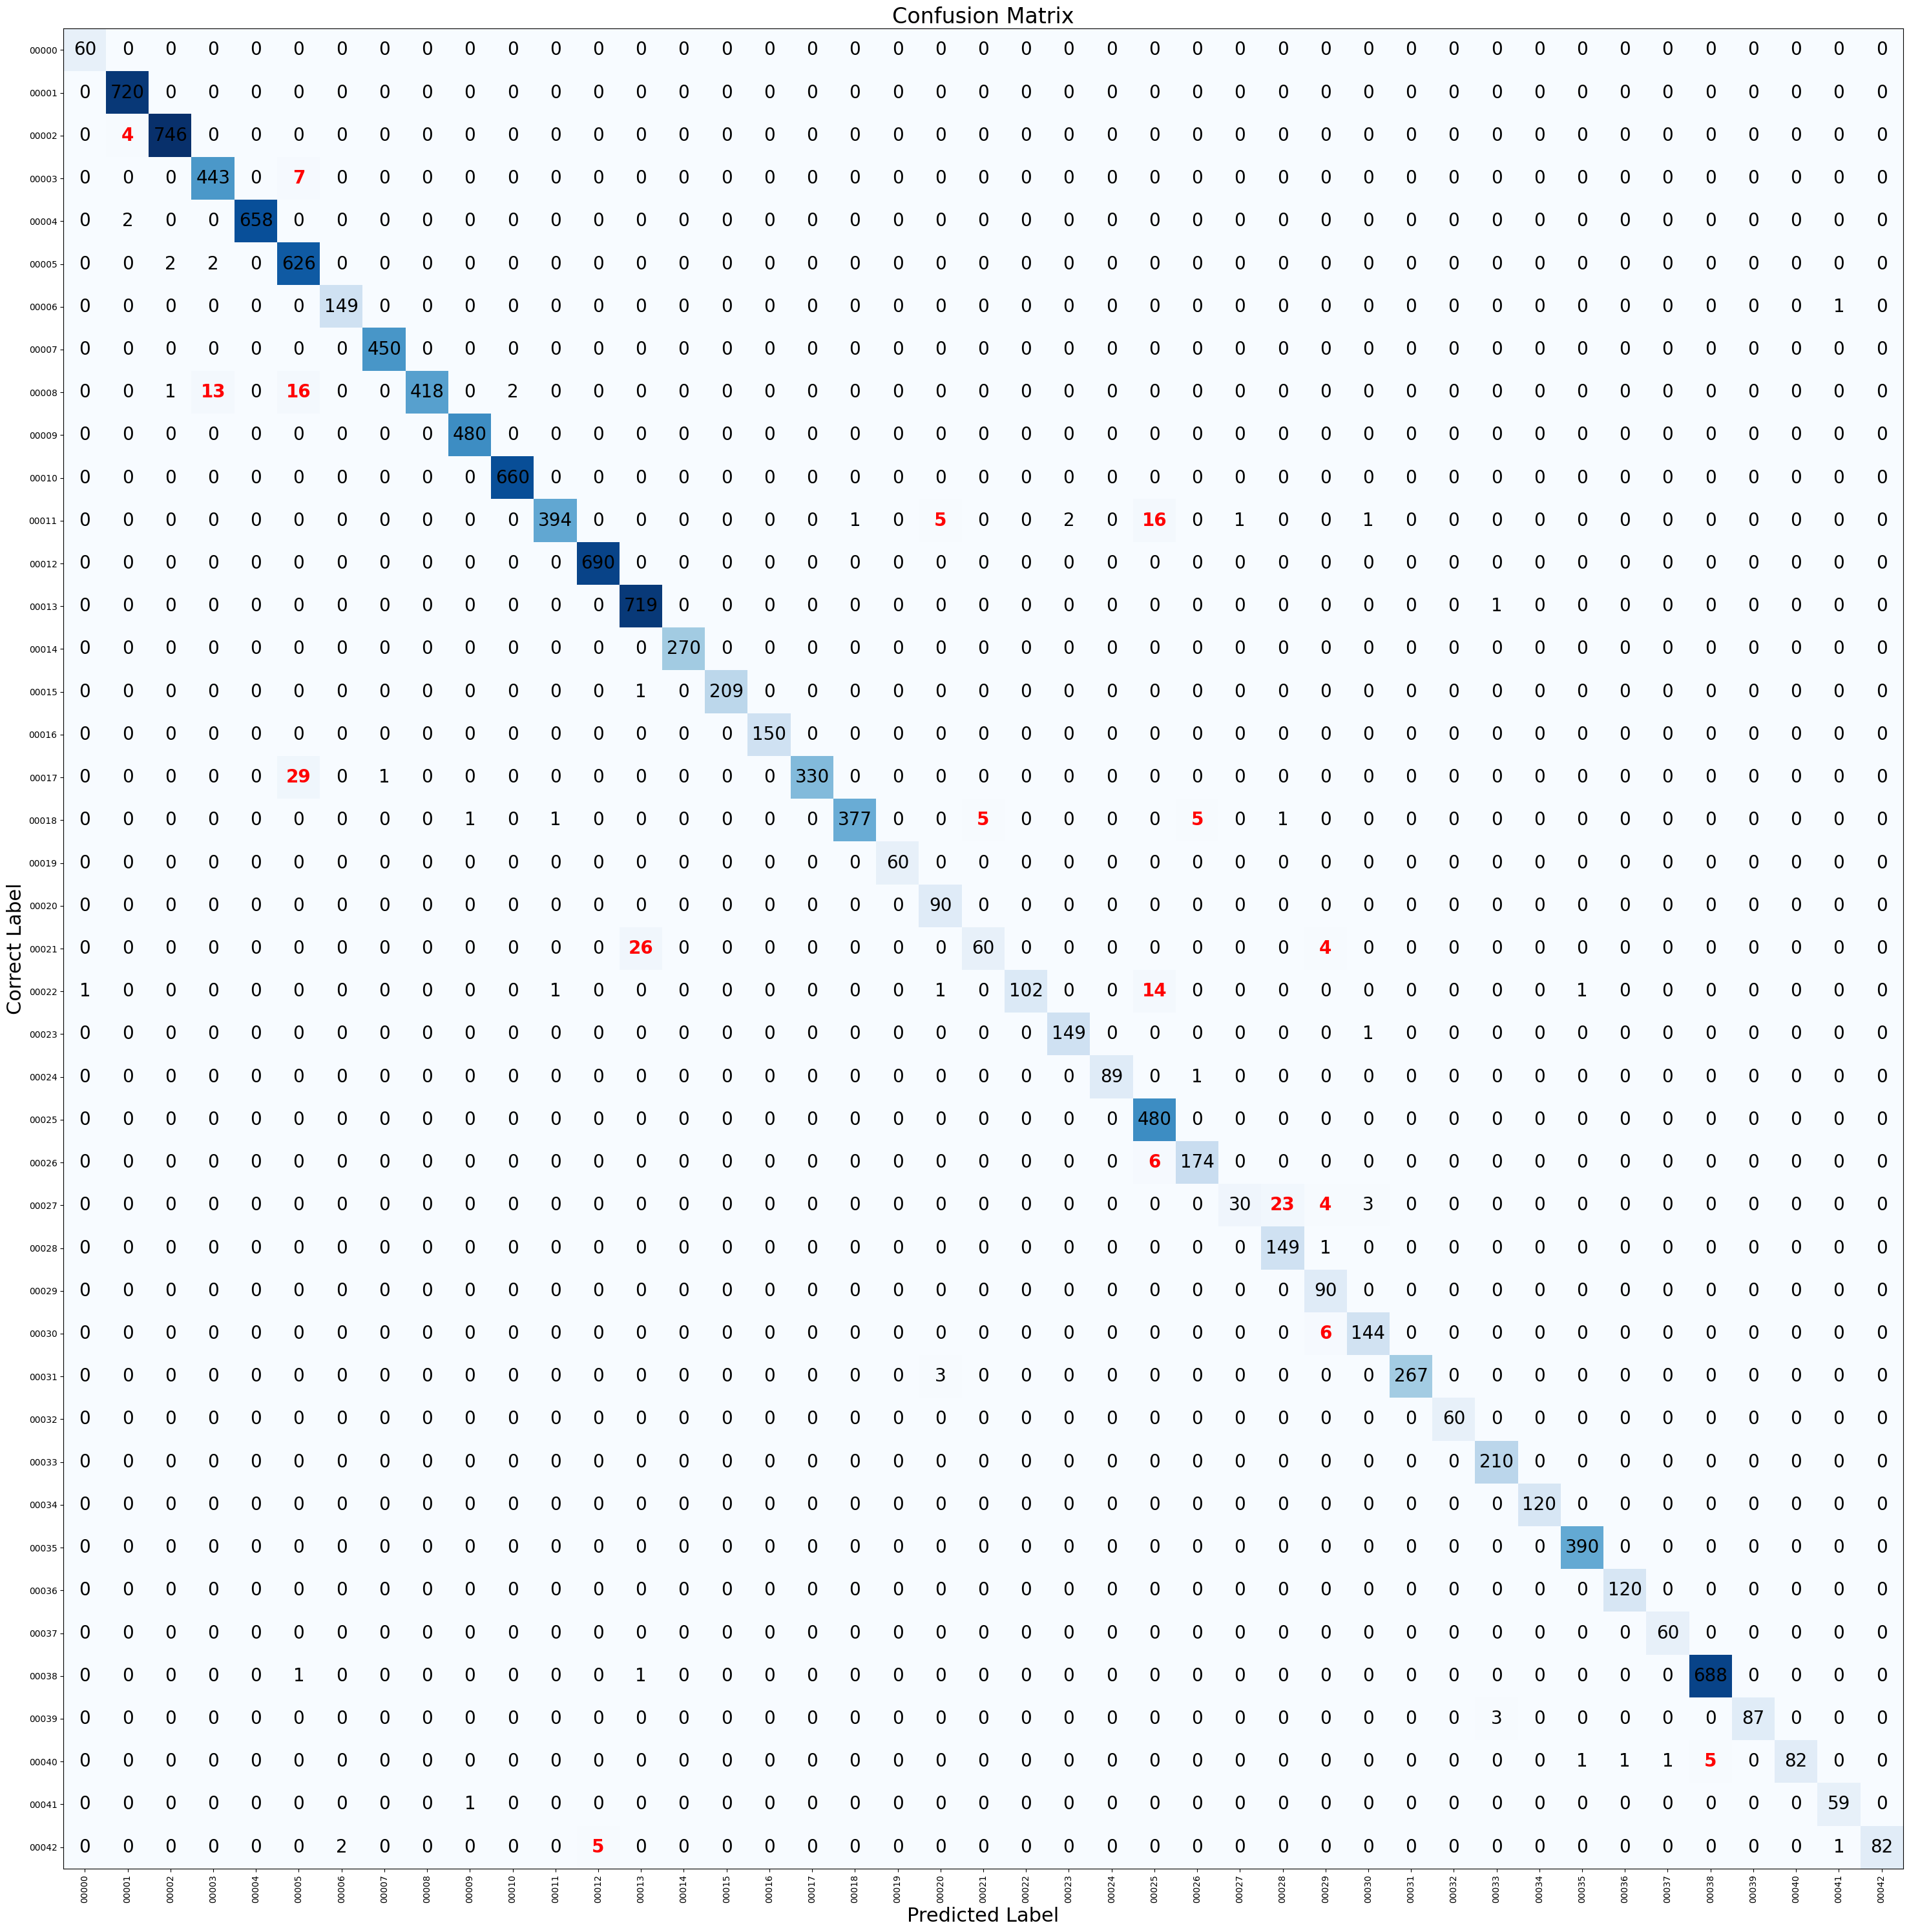
\includegraphics[width=0.8\linewidth]{images/gaussianblur_confusion_matrix.png}
    \caption{Dynamic Gaussian Blur confusion matrix.}
    \label{fig:gaussianblur_confusion_matrix}
\end{figure}

\begin{figure}[h]
    \centering
    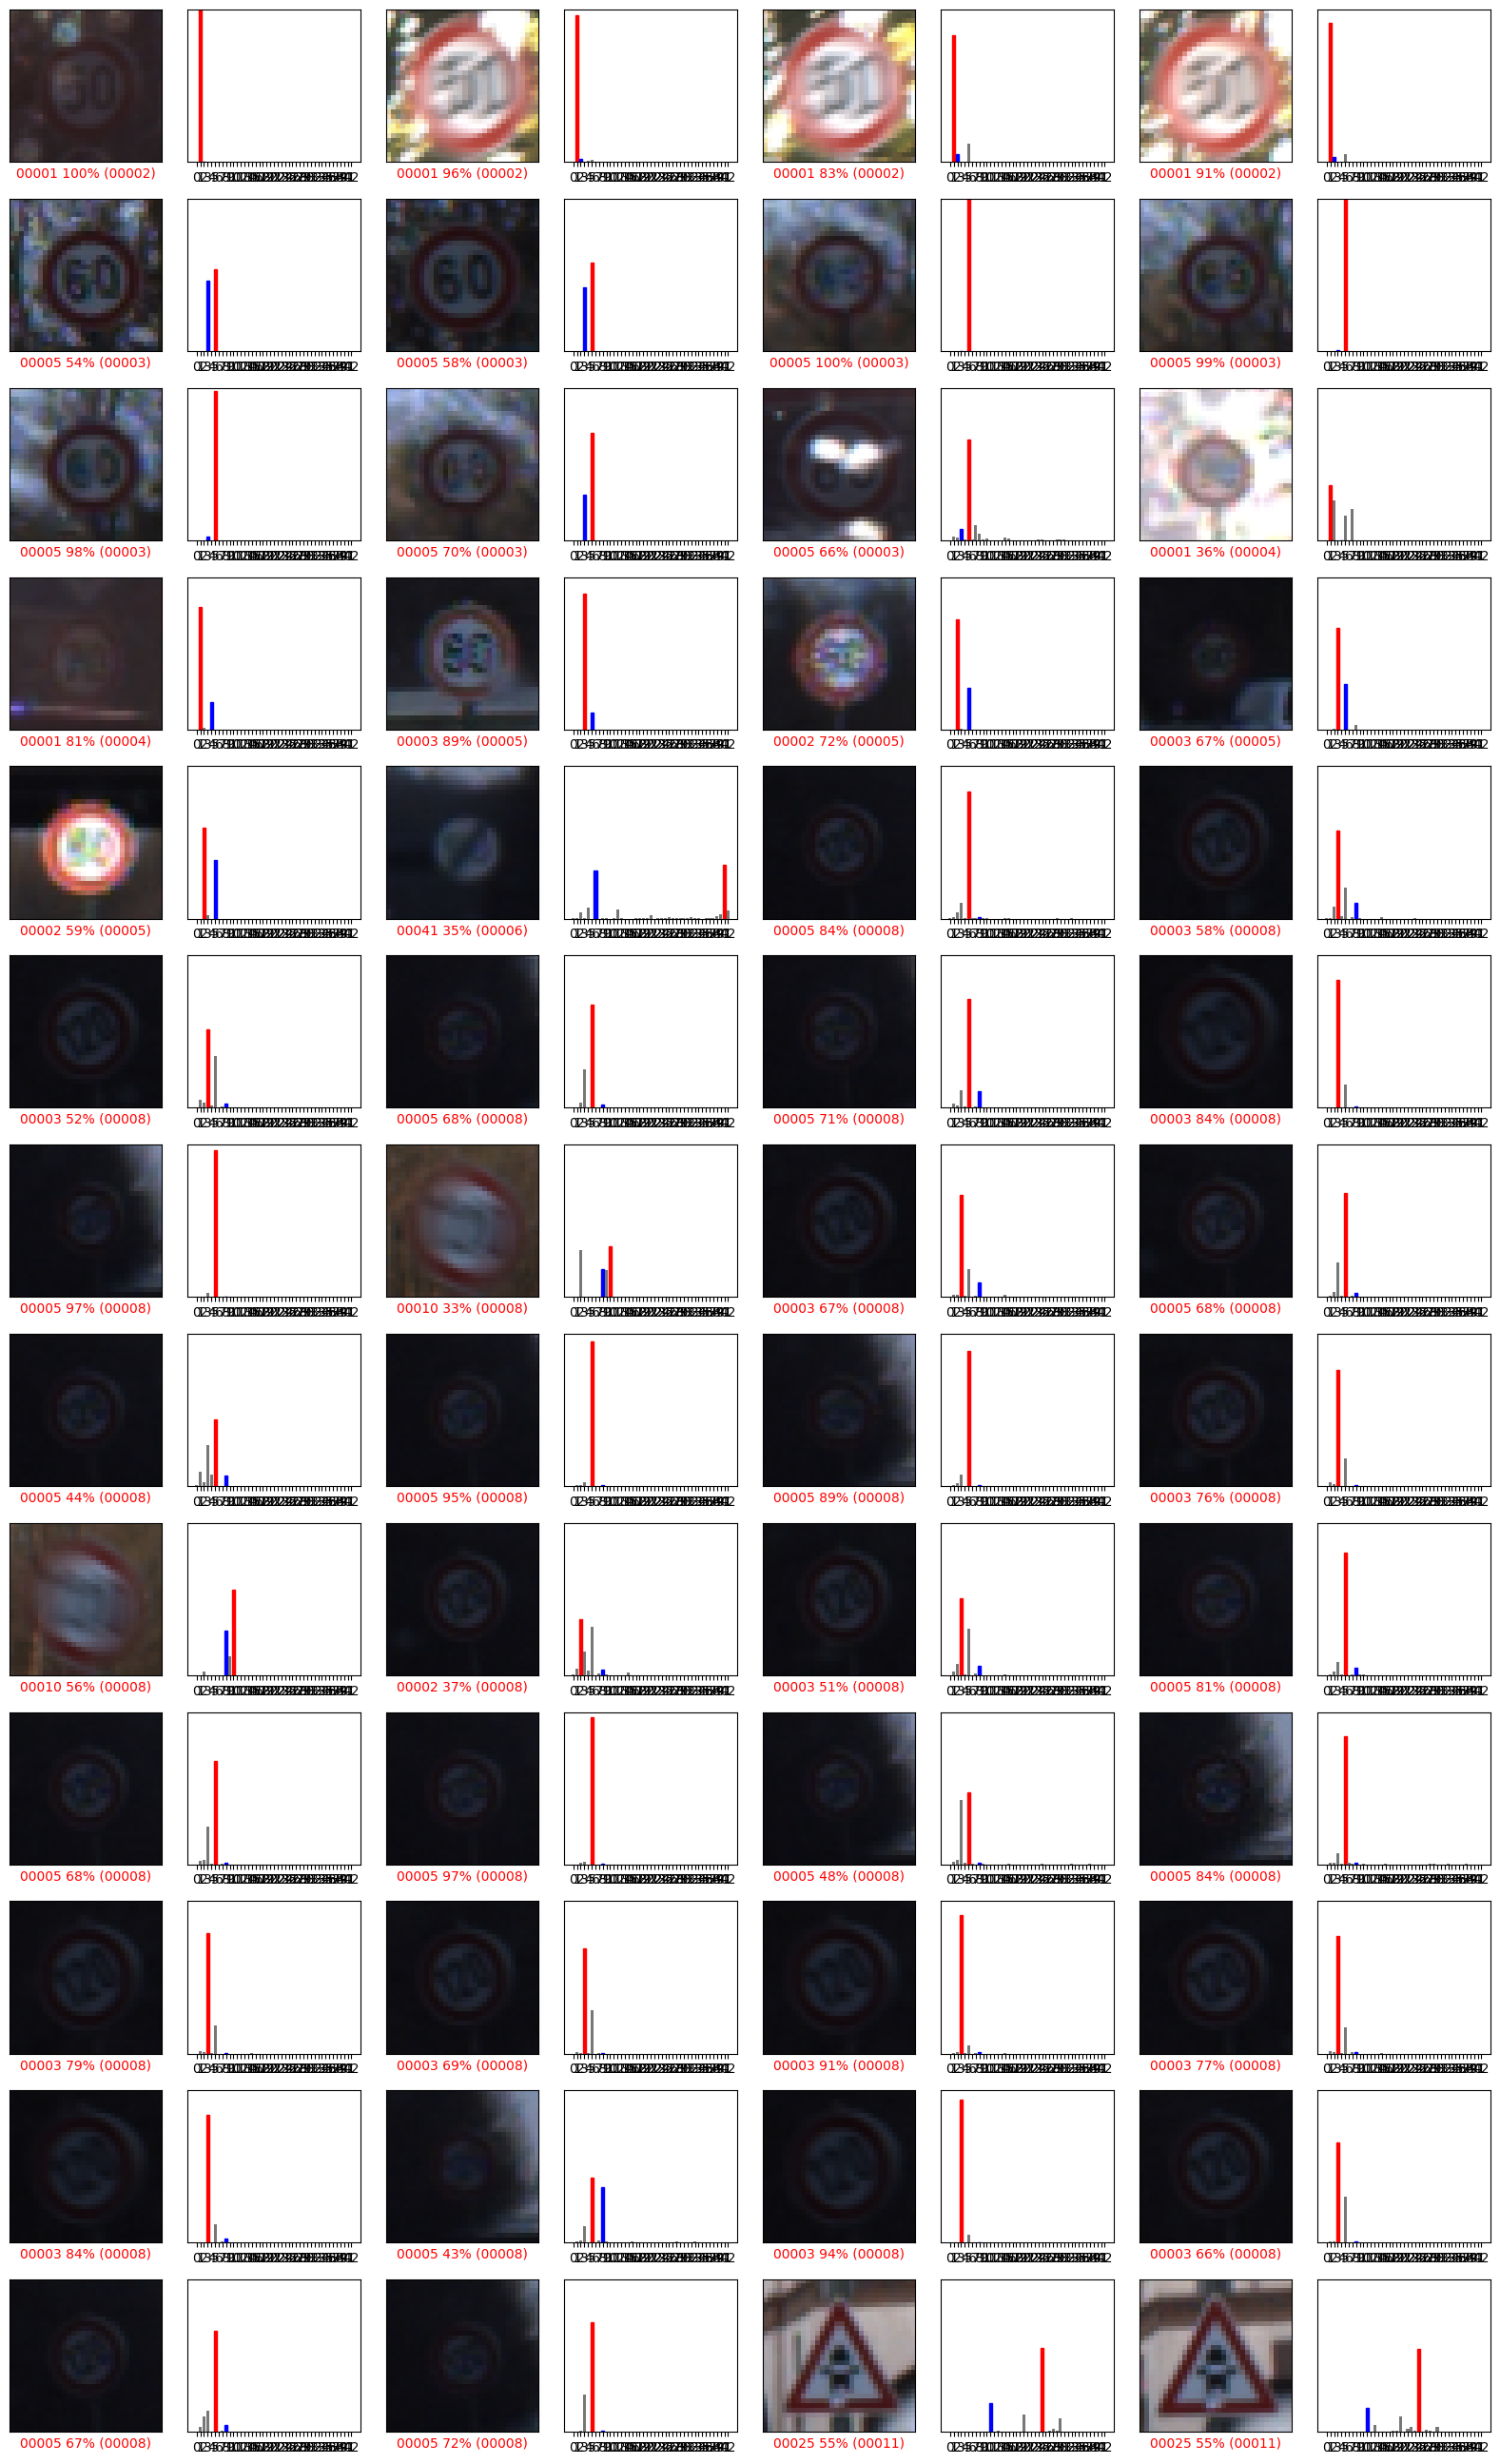
\includegraphics[width=0.8\linewidth]{images/gaussianblur_bad_predictions.png}
    \caption{Dynamic Gaussian Blur misclassified samples.}
    \label{fig:gaussianblur_bad_predictions}
\end{figure}

\subsubsection{Random Erasing}

\begin{figure}[h]
    \centering
    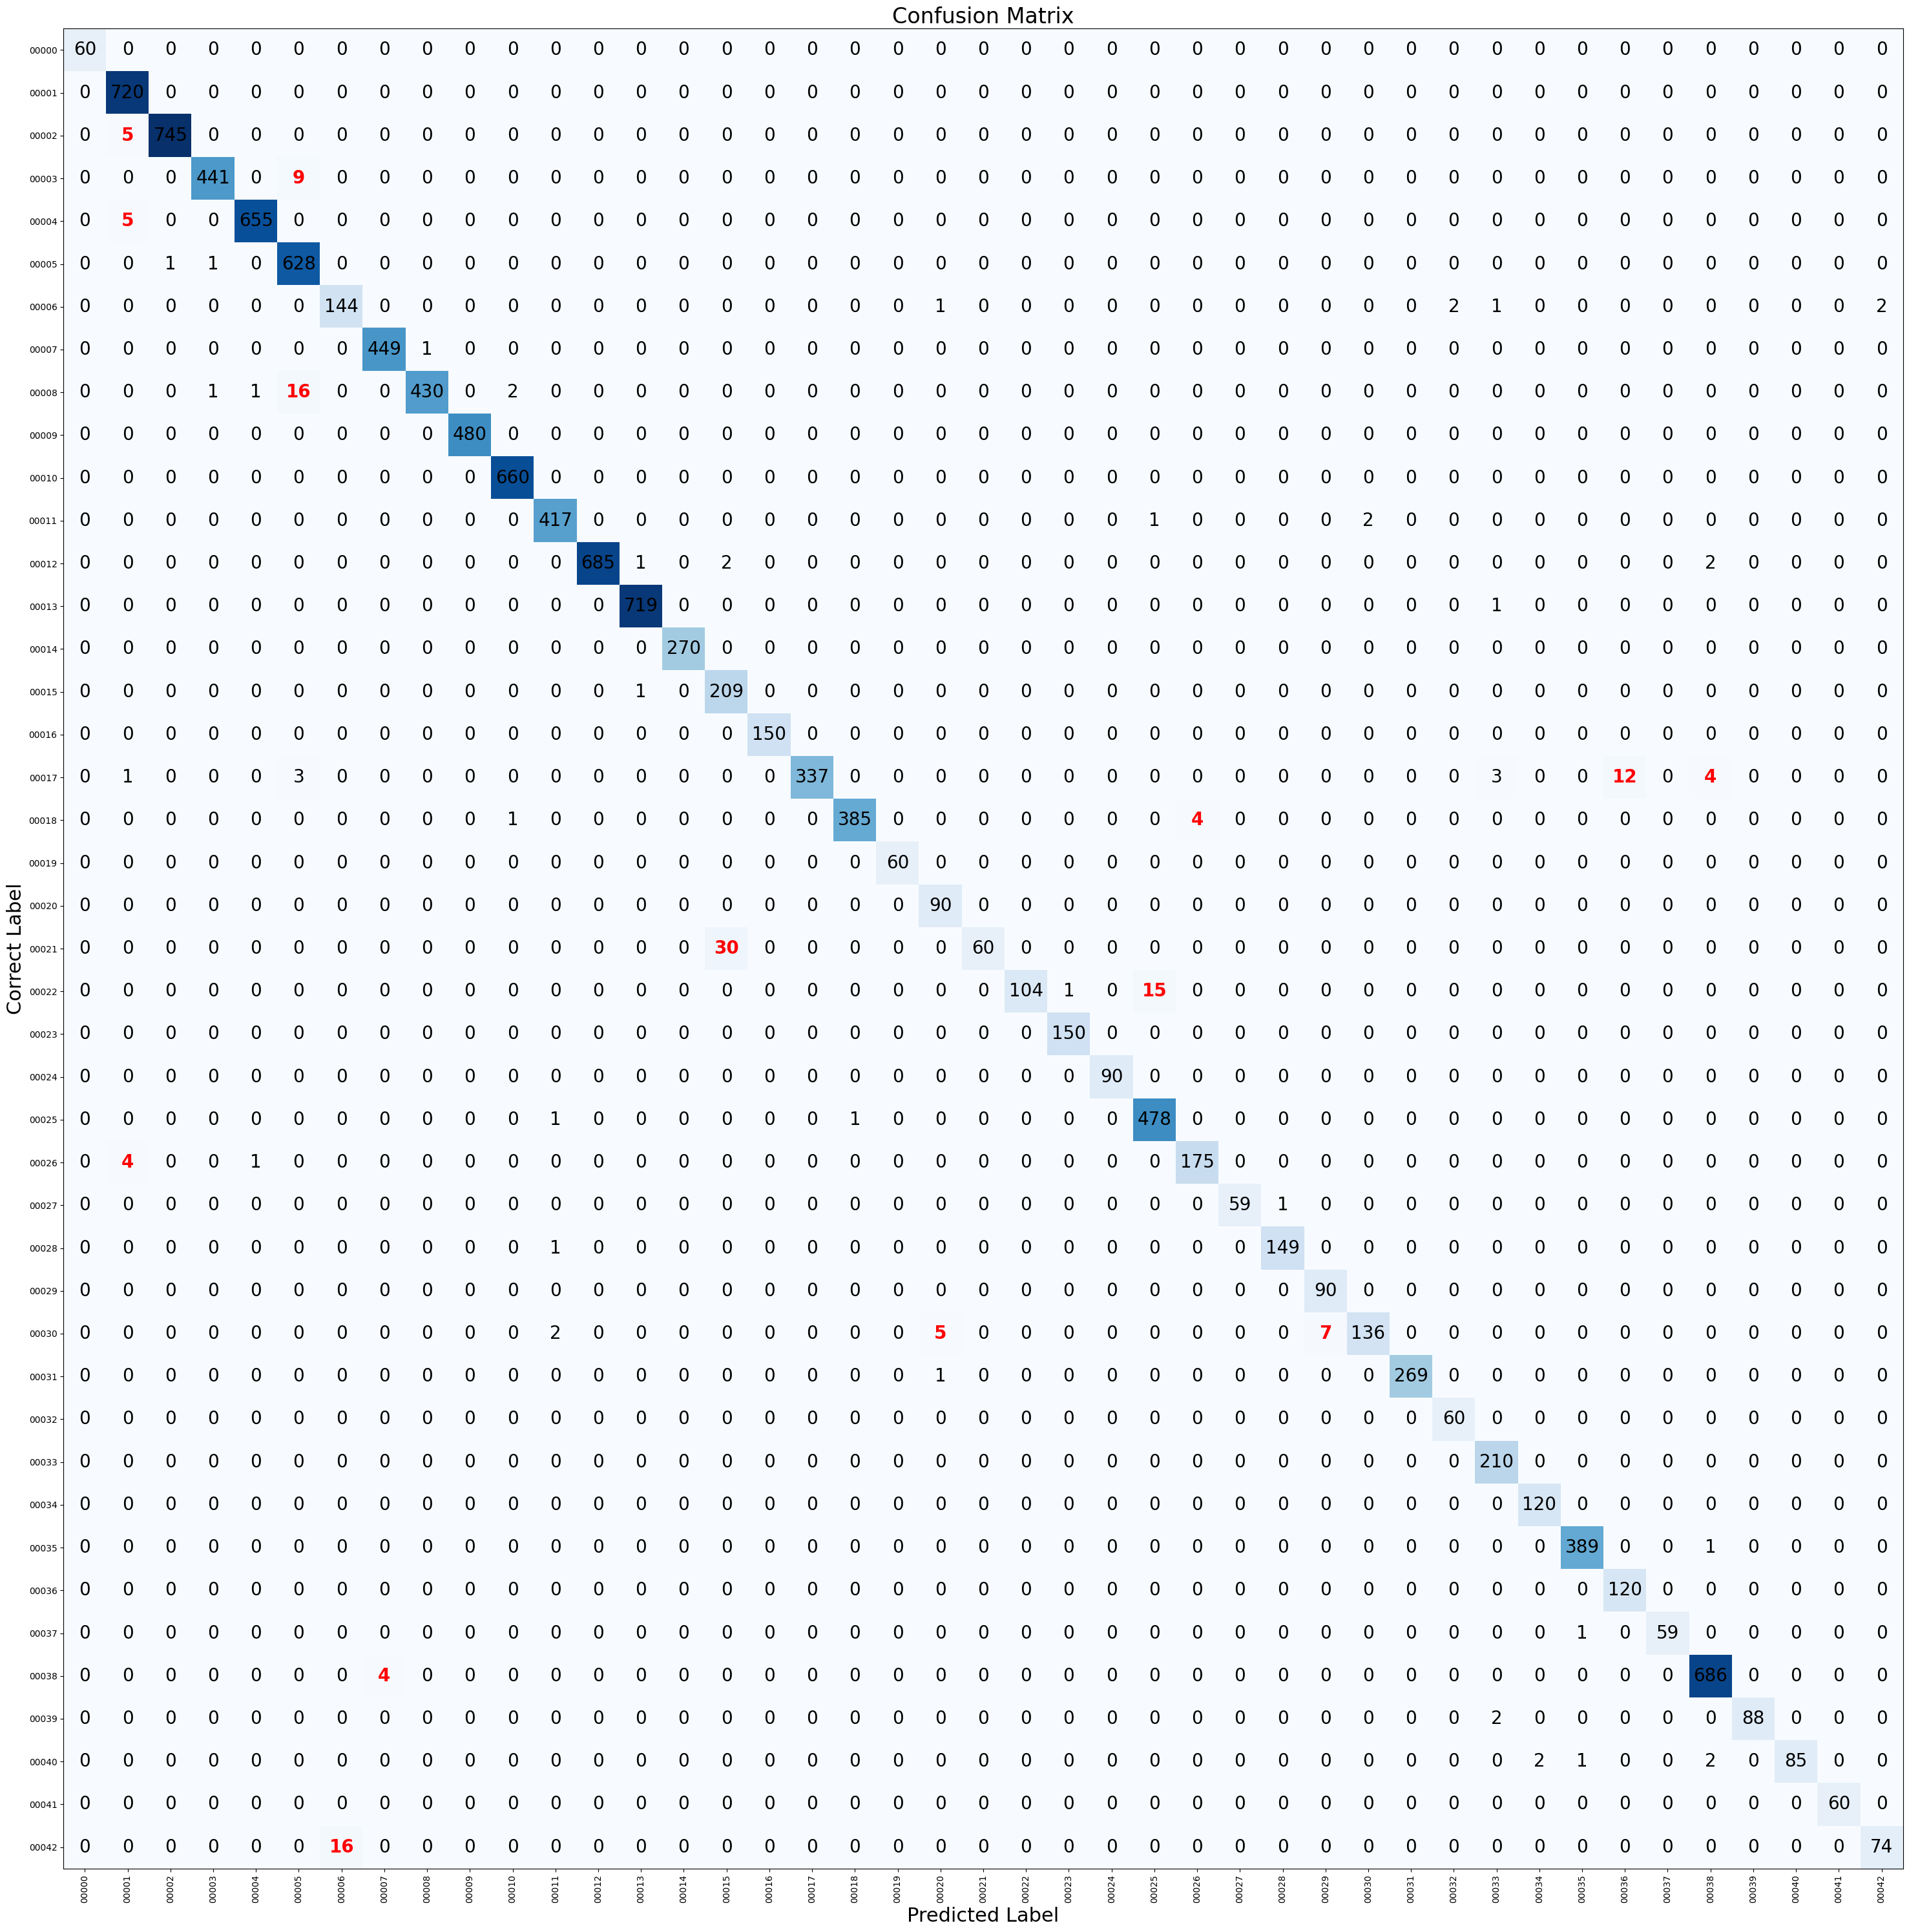
\includegraphics[width=0.8\linewidth]{images/random_erasing_confusion_matrix.png}
    \caption{Dynamic Random Erasing confusion matrix.}
    \label{fig:random_erasing_confusion_matrix}
\end{figure}

\begin{figure}[h]
    \centering
    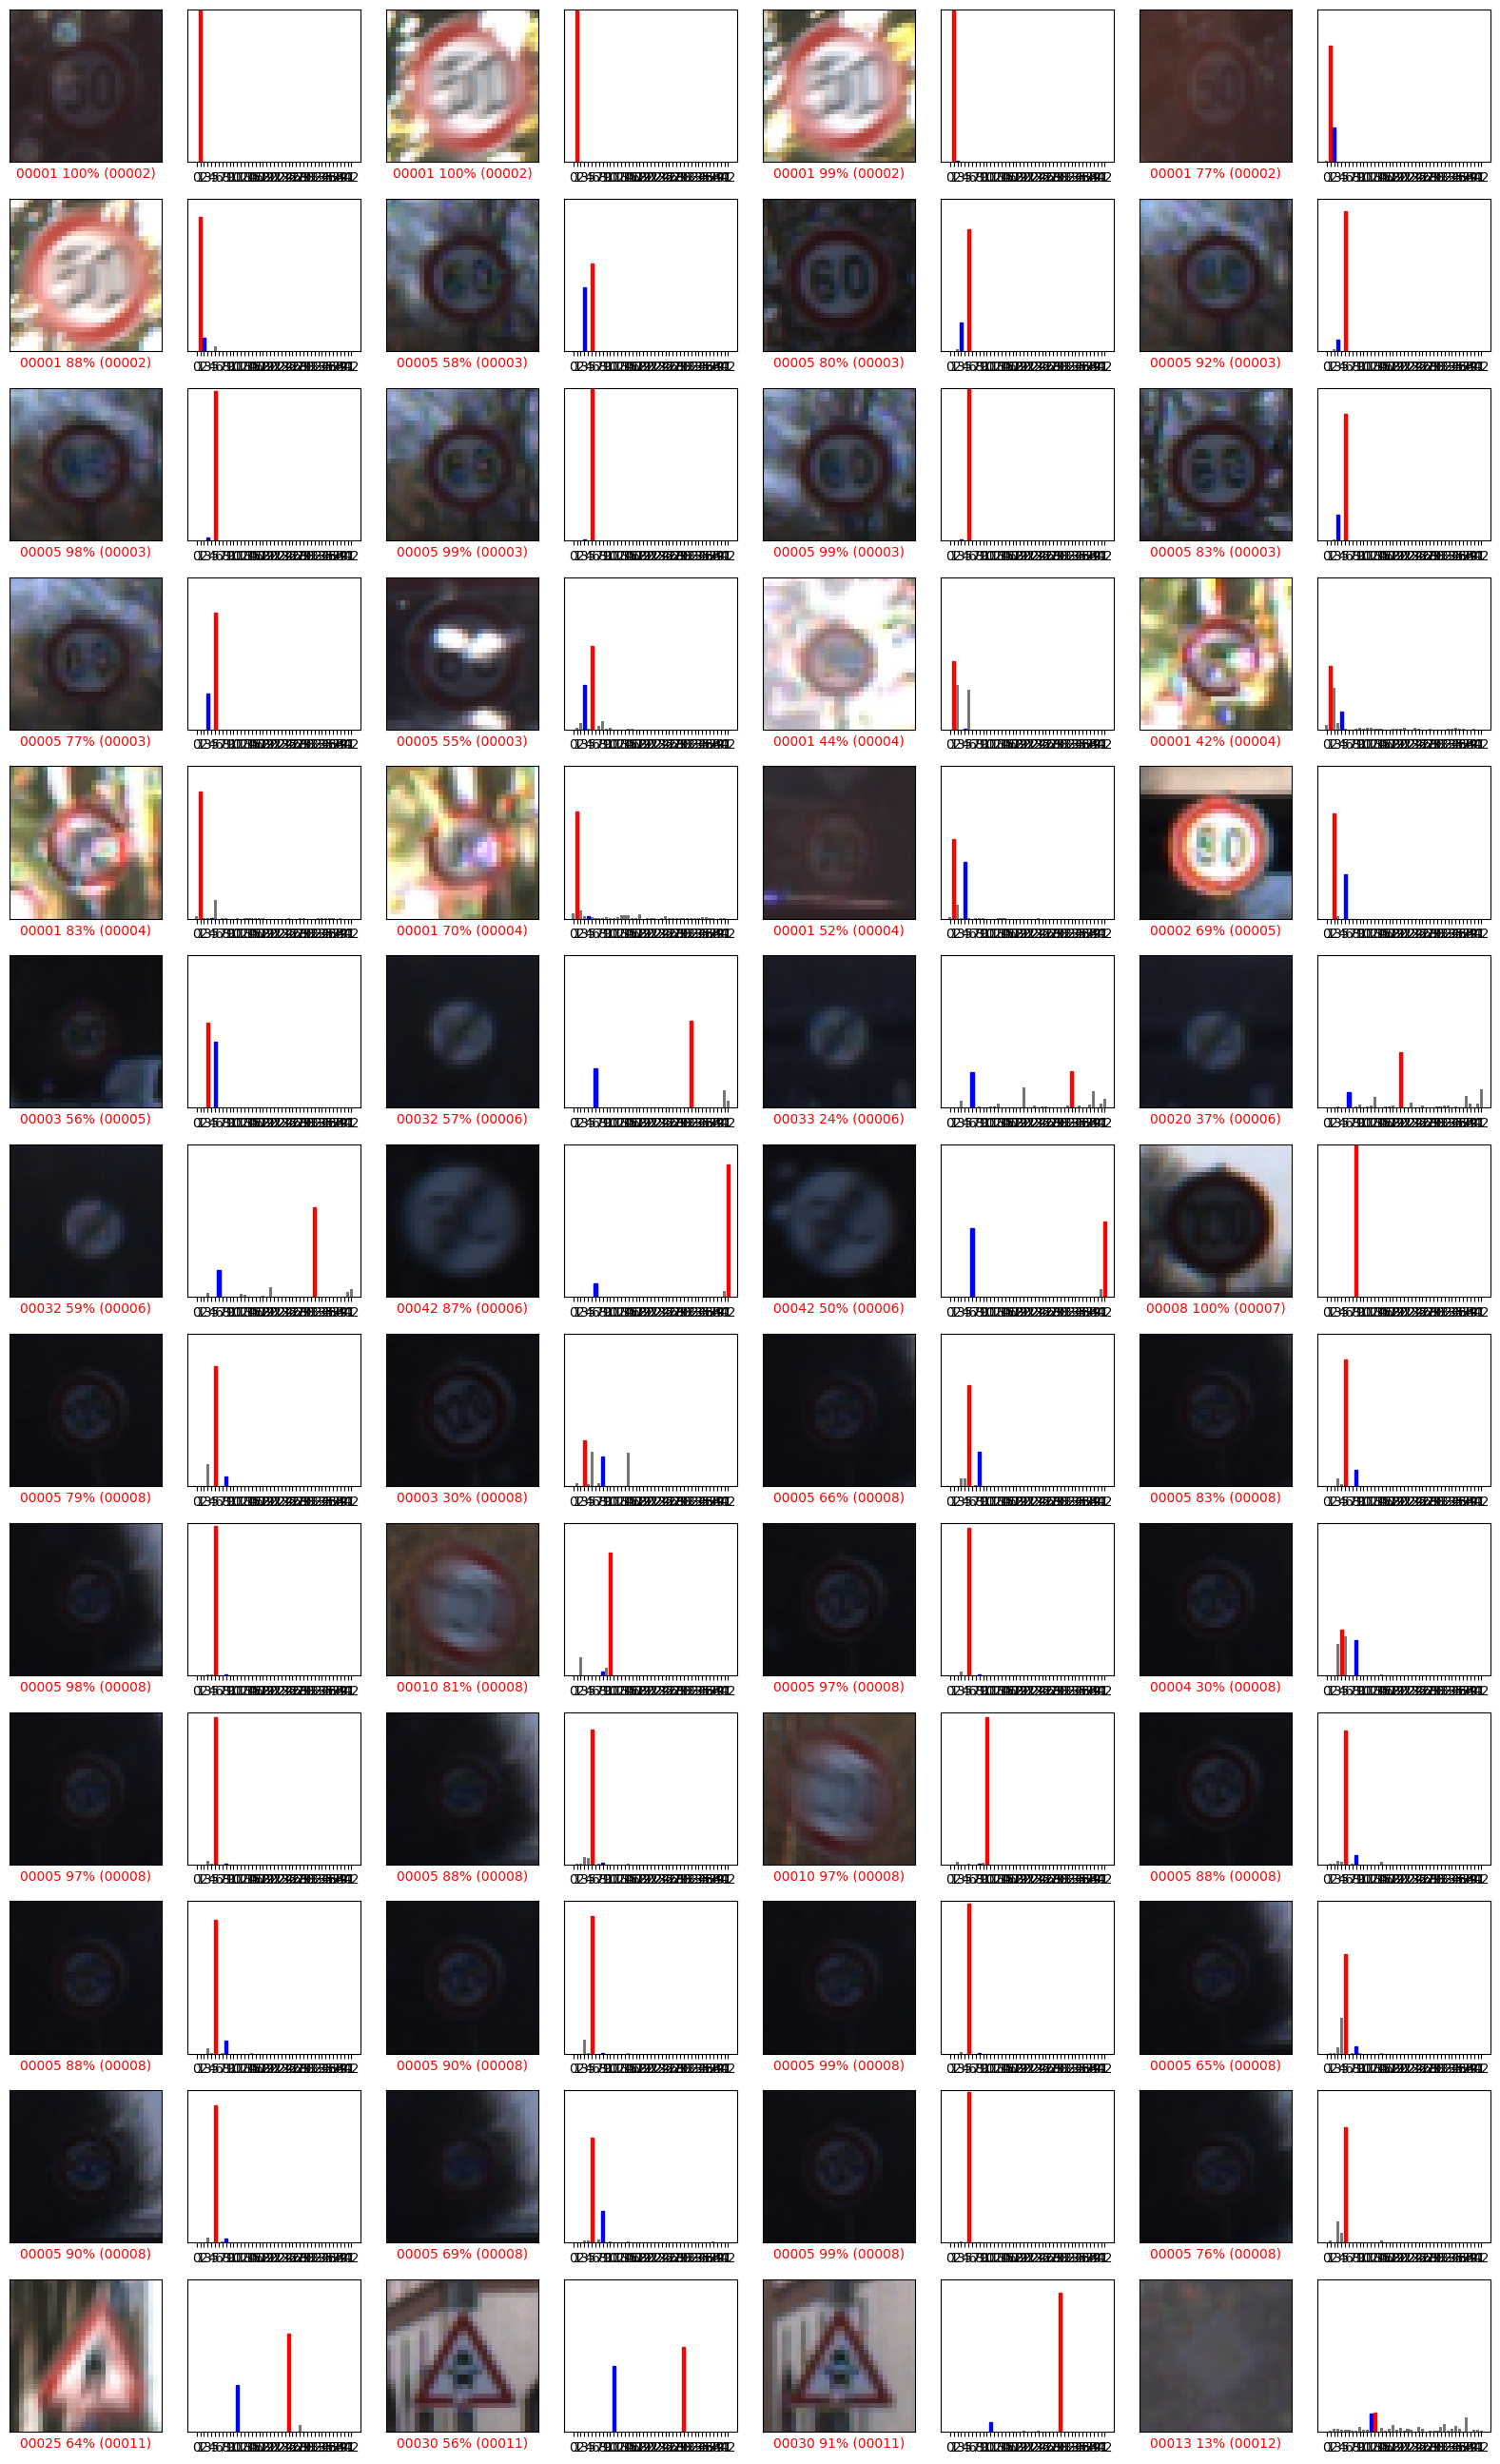
\includegraphics[width=0.8\linewidth]{images/random_erasing_bad_predictions.png}
    \caption{Dynamic Random Erasing misclassified samples.}
    \label{fig:random_erasing_bad_predictions}
\end{figure}

\subsubsection{Combined Dynamic}

\begin{figure}[h]
    \centering
    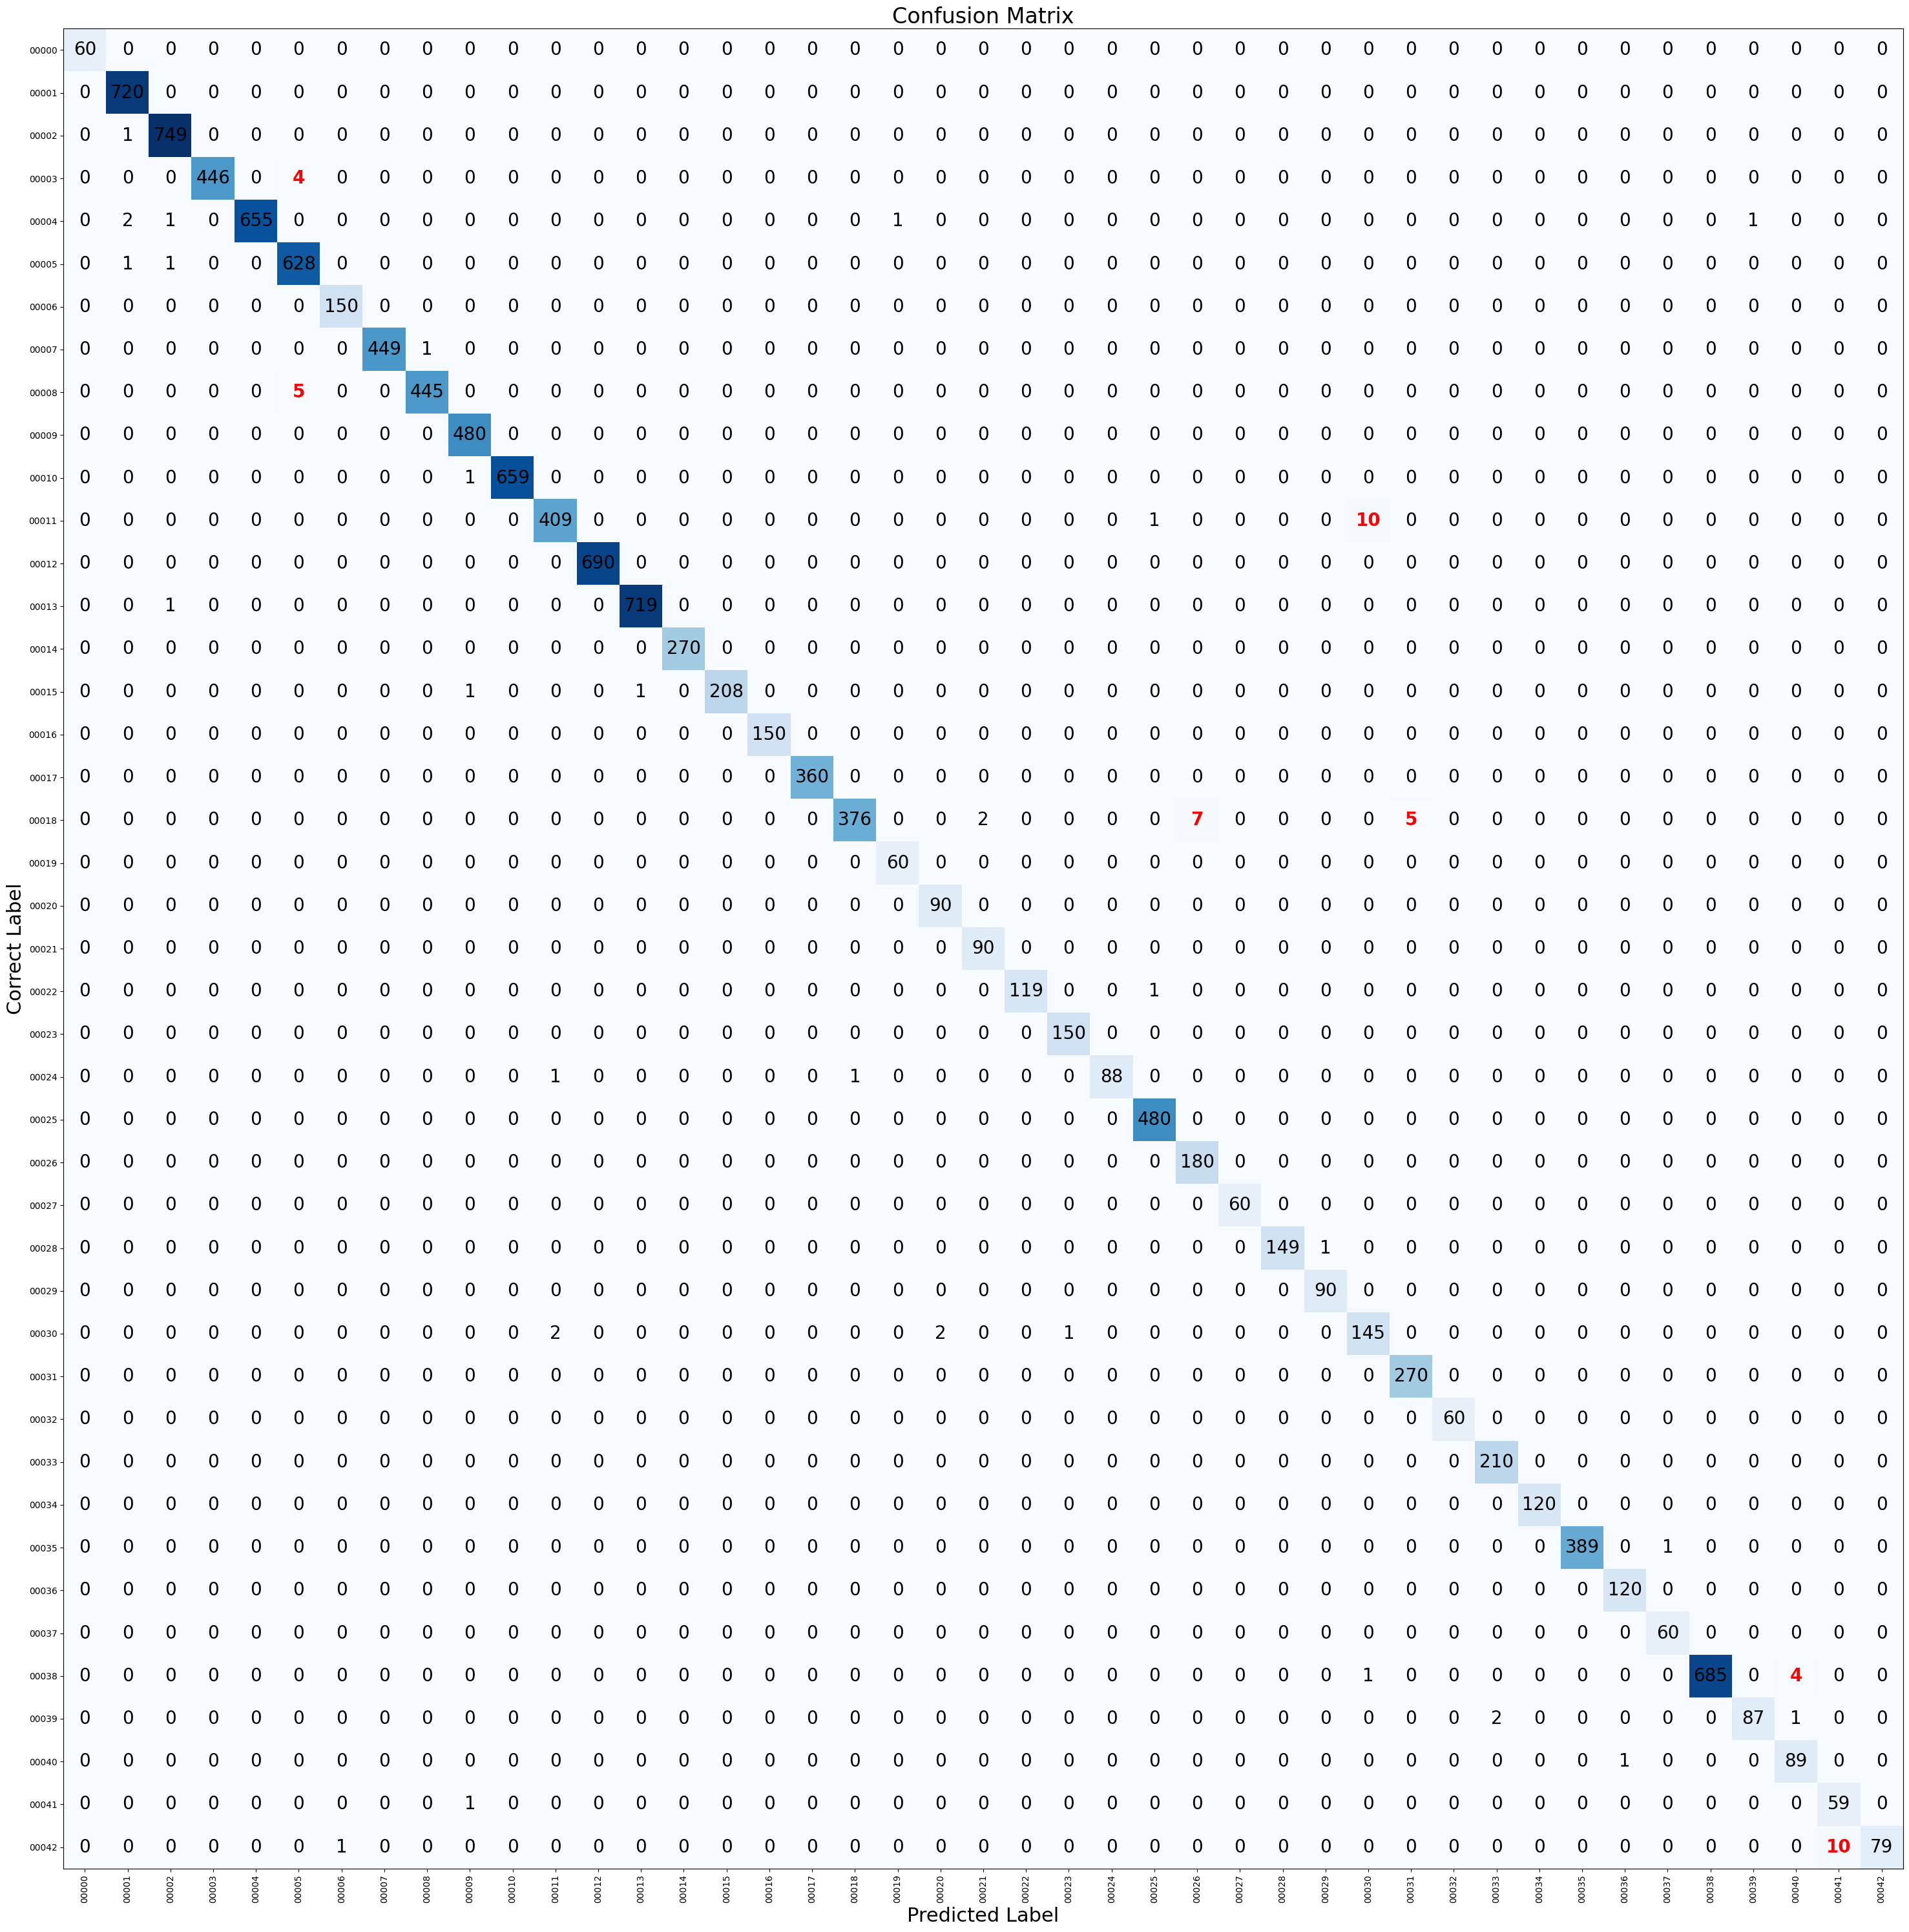
\includegraphics[width=0.8\linewidth]{images/combined_confusion_matrix.png}
    \caption{Combined dynamic augmentation confusion matrix.}
    \label{fig:combined_confusion_matrix}
\end{figure}

\begin{figure}[h]
    \centering
    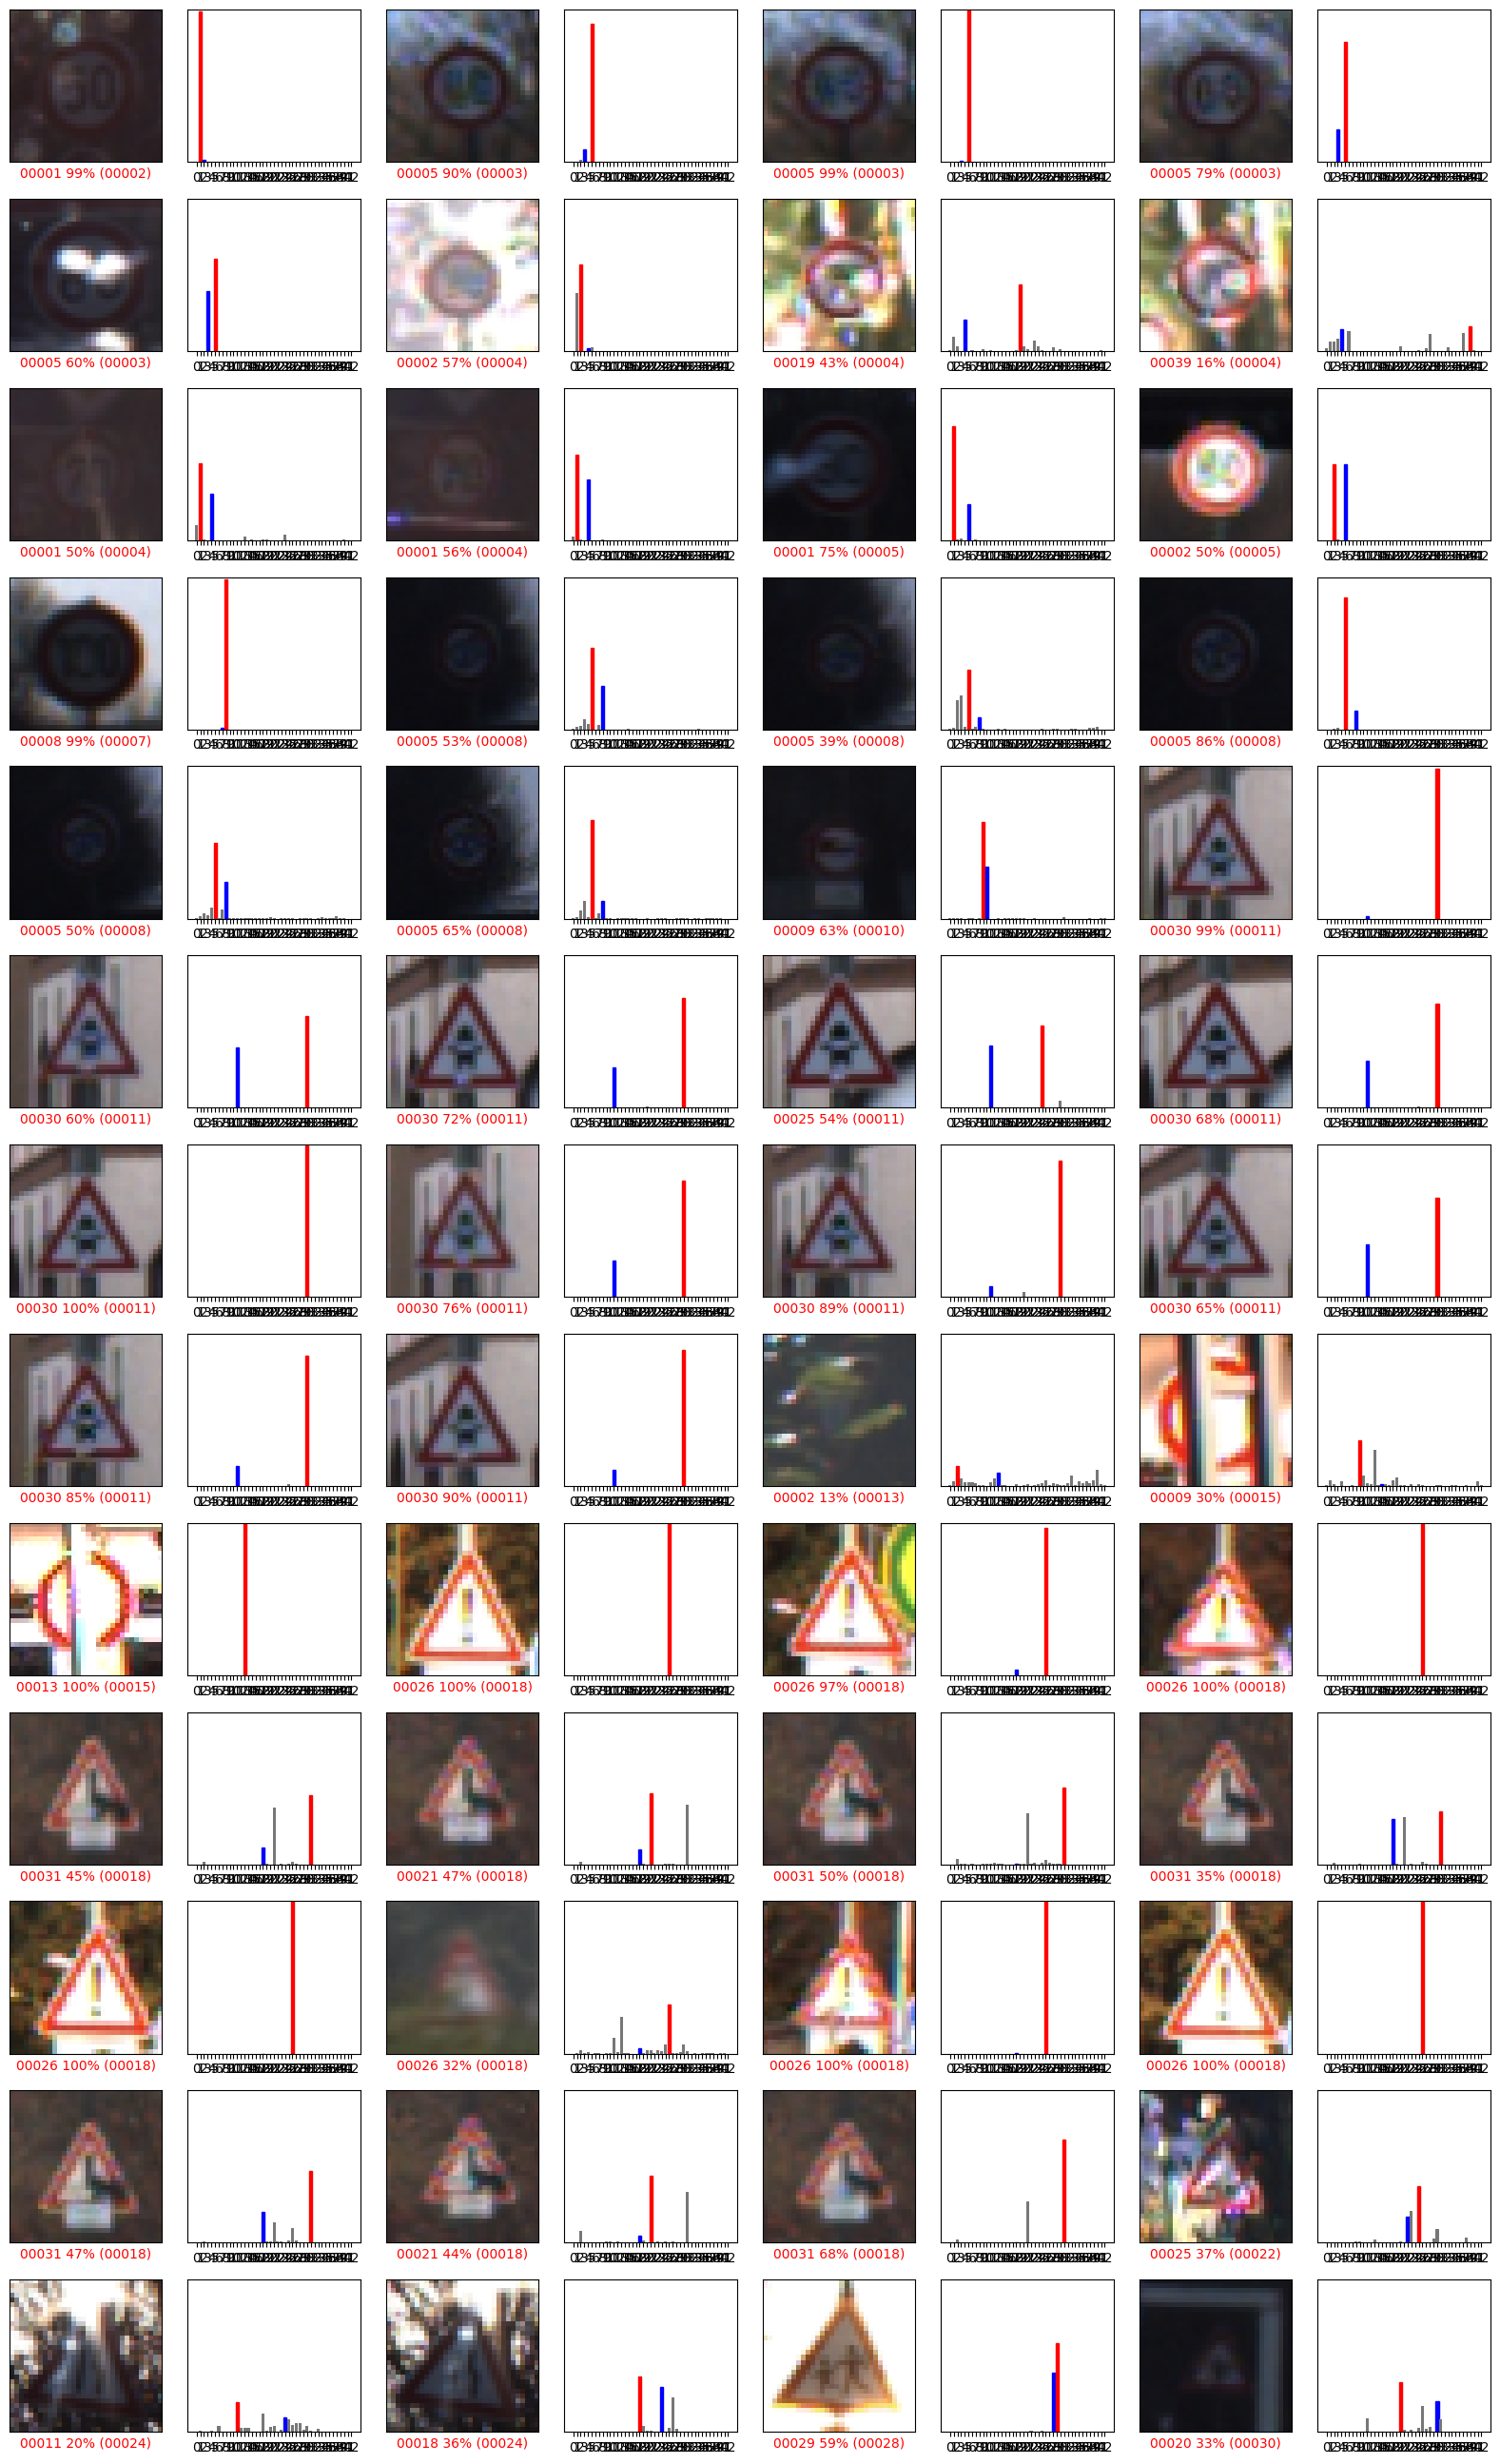
\includegraphics[width=0.8\linewidth]{images/combined_bad_predictions.png}
    \caption{Combined dynamic augmentation misclassified samples.}
    \label{fig:combined_bad_predictions}
\end{figure}

\subsection{Static Models}

\subsubsection{ColorJitter}

\begin{figure}[h]
    \centering
    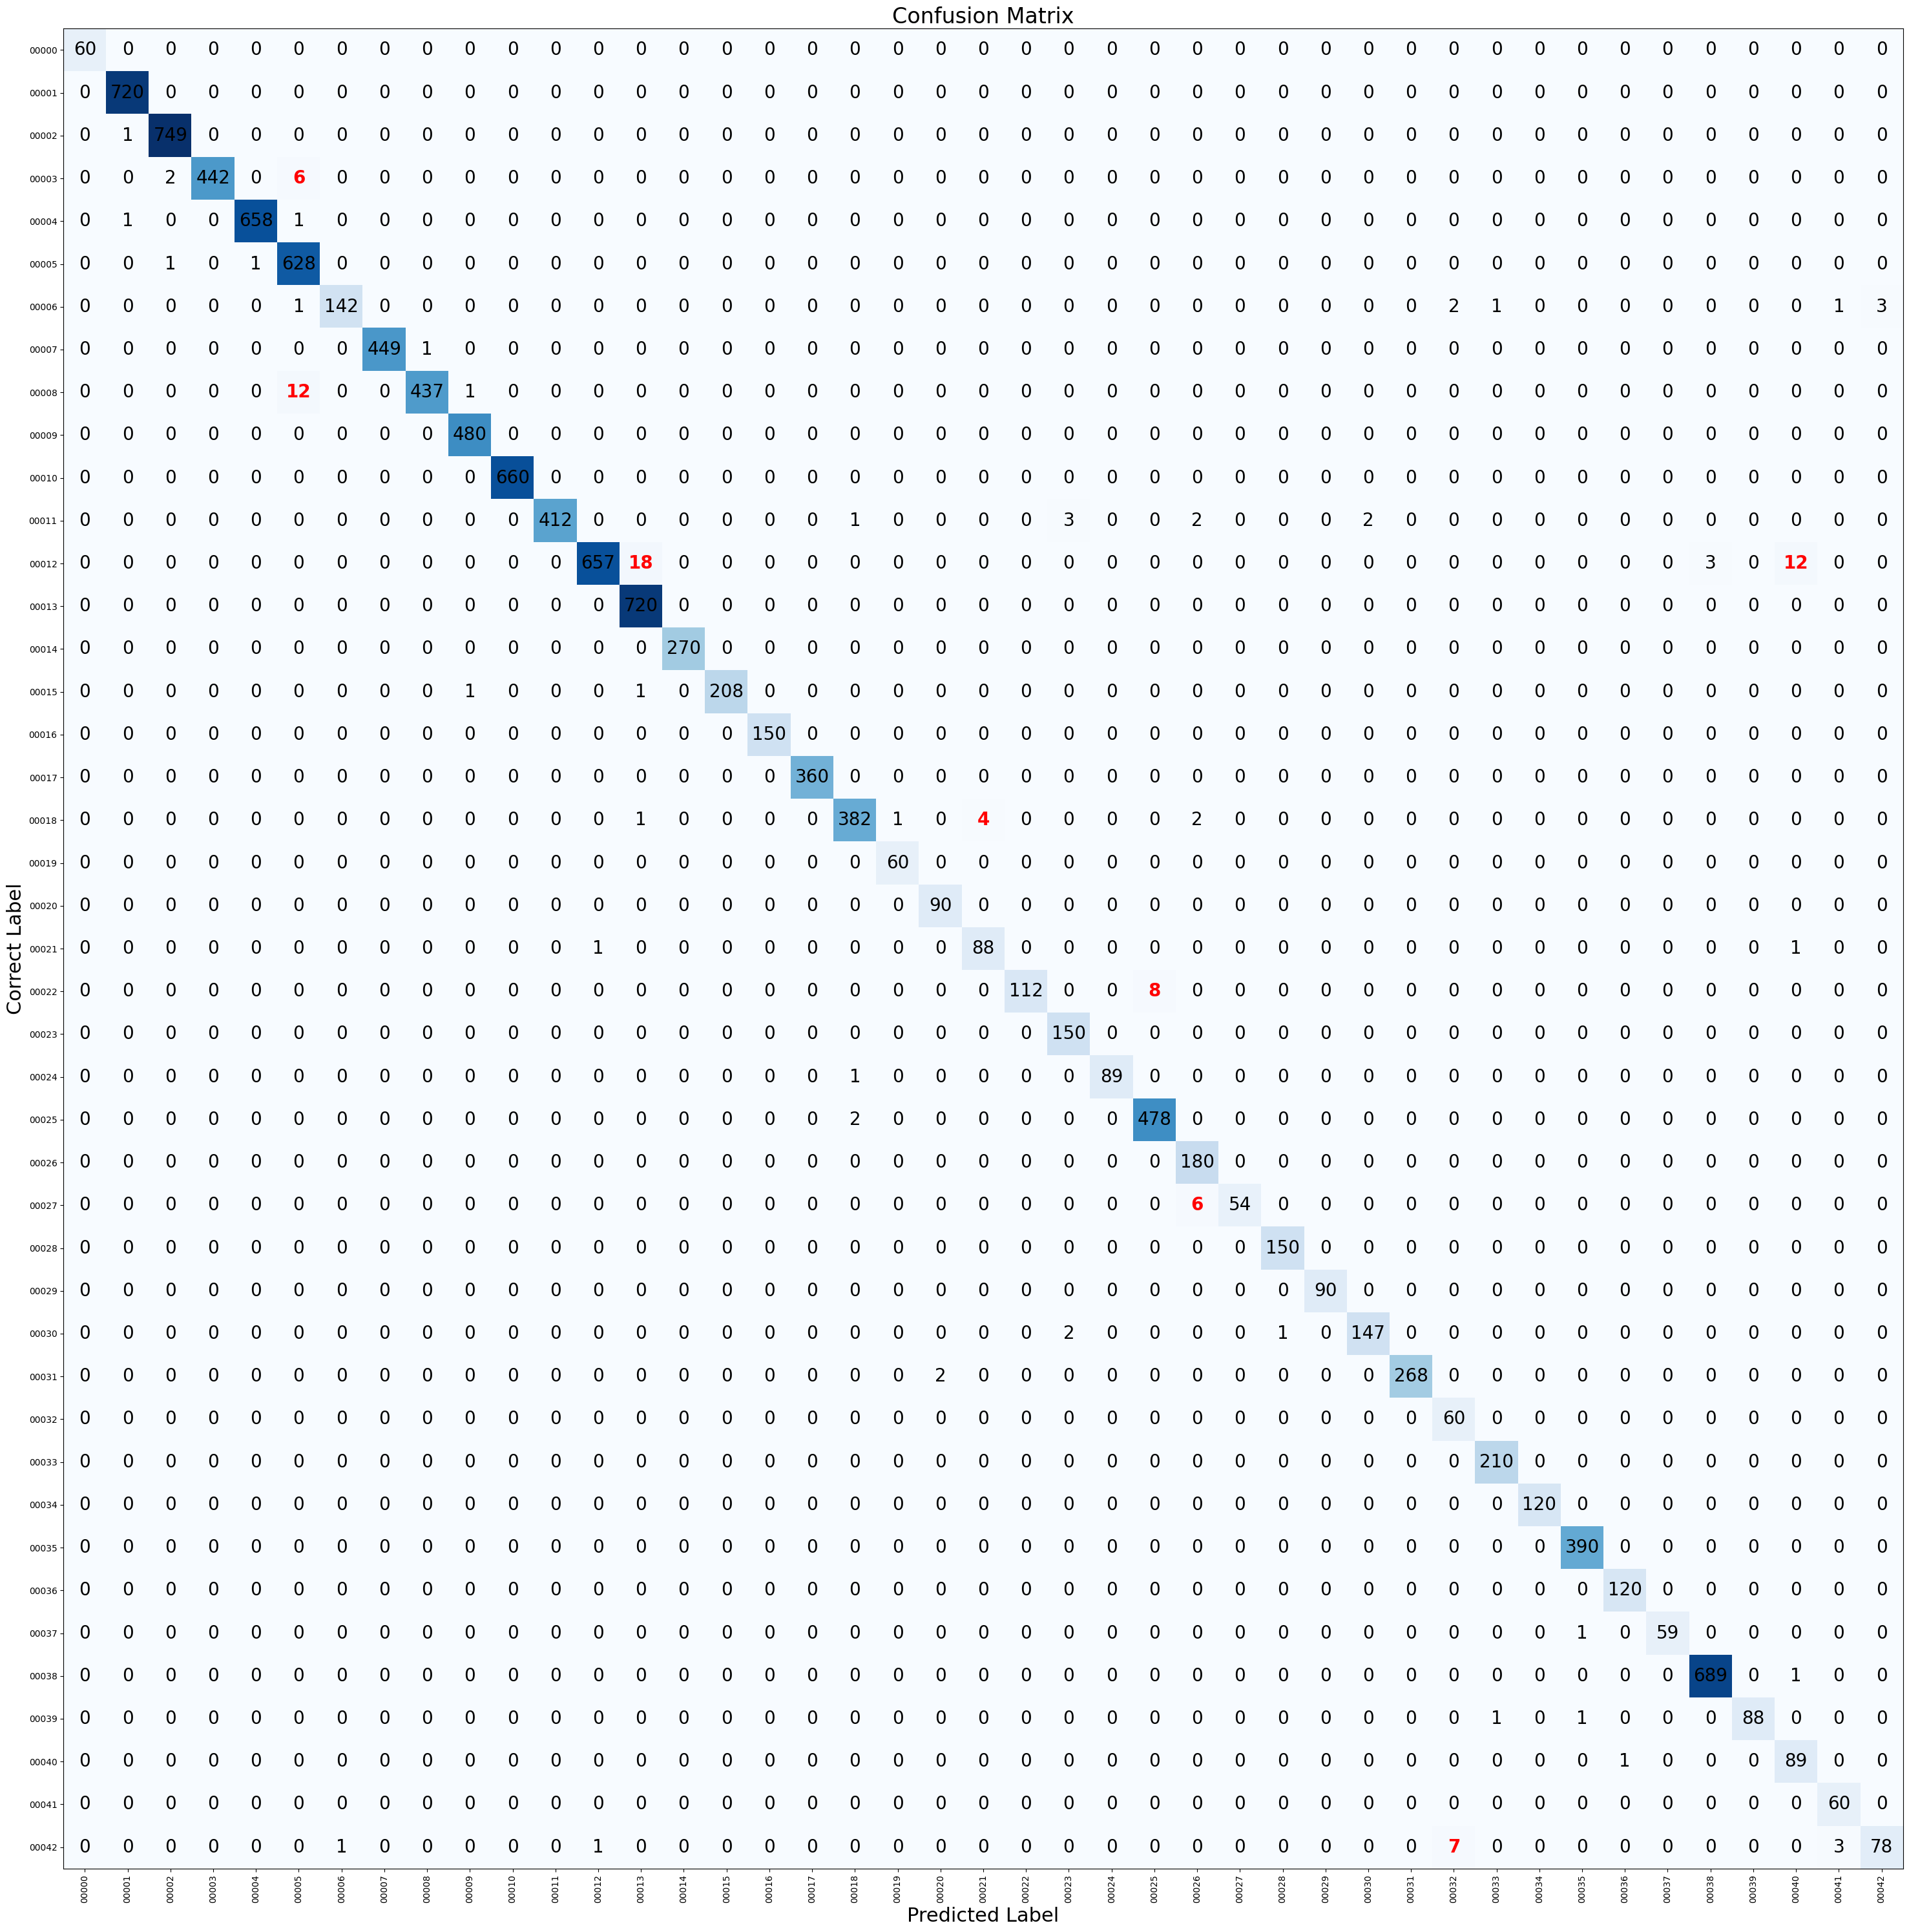
\includegraphics[width=0.8\linewidth]{images/static_colorjitter_confusion_matrix.png}
    \caption{Static ColorJitter confusion matrix.}
    \label{fig:static_colorjitter_confusion_matrix}
\end{figure}

\begin{figure}[h]
    \centering
    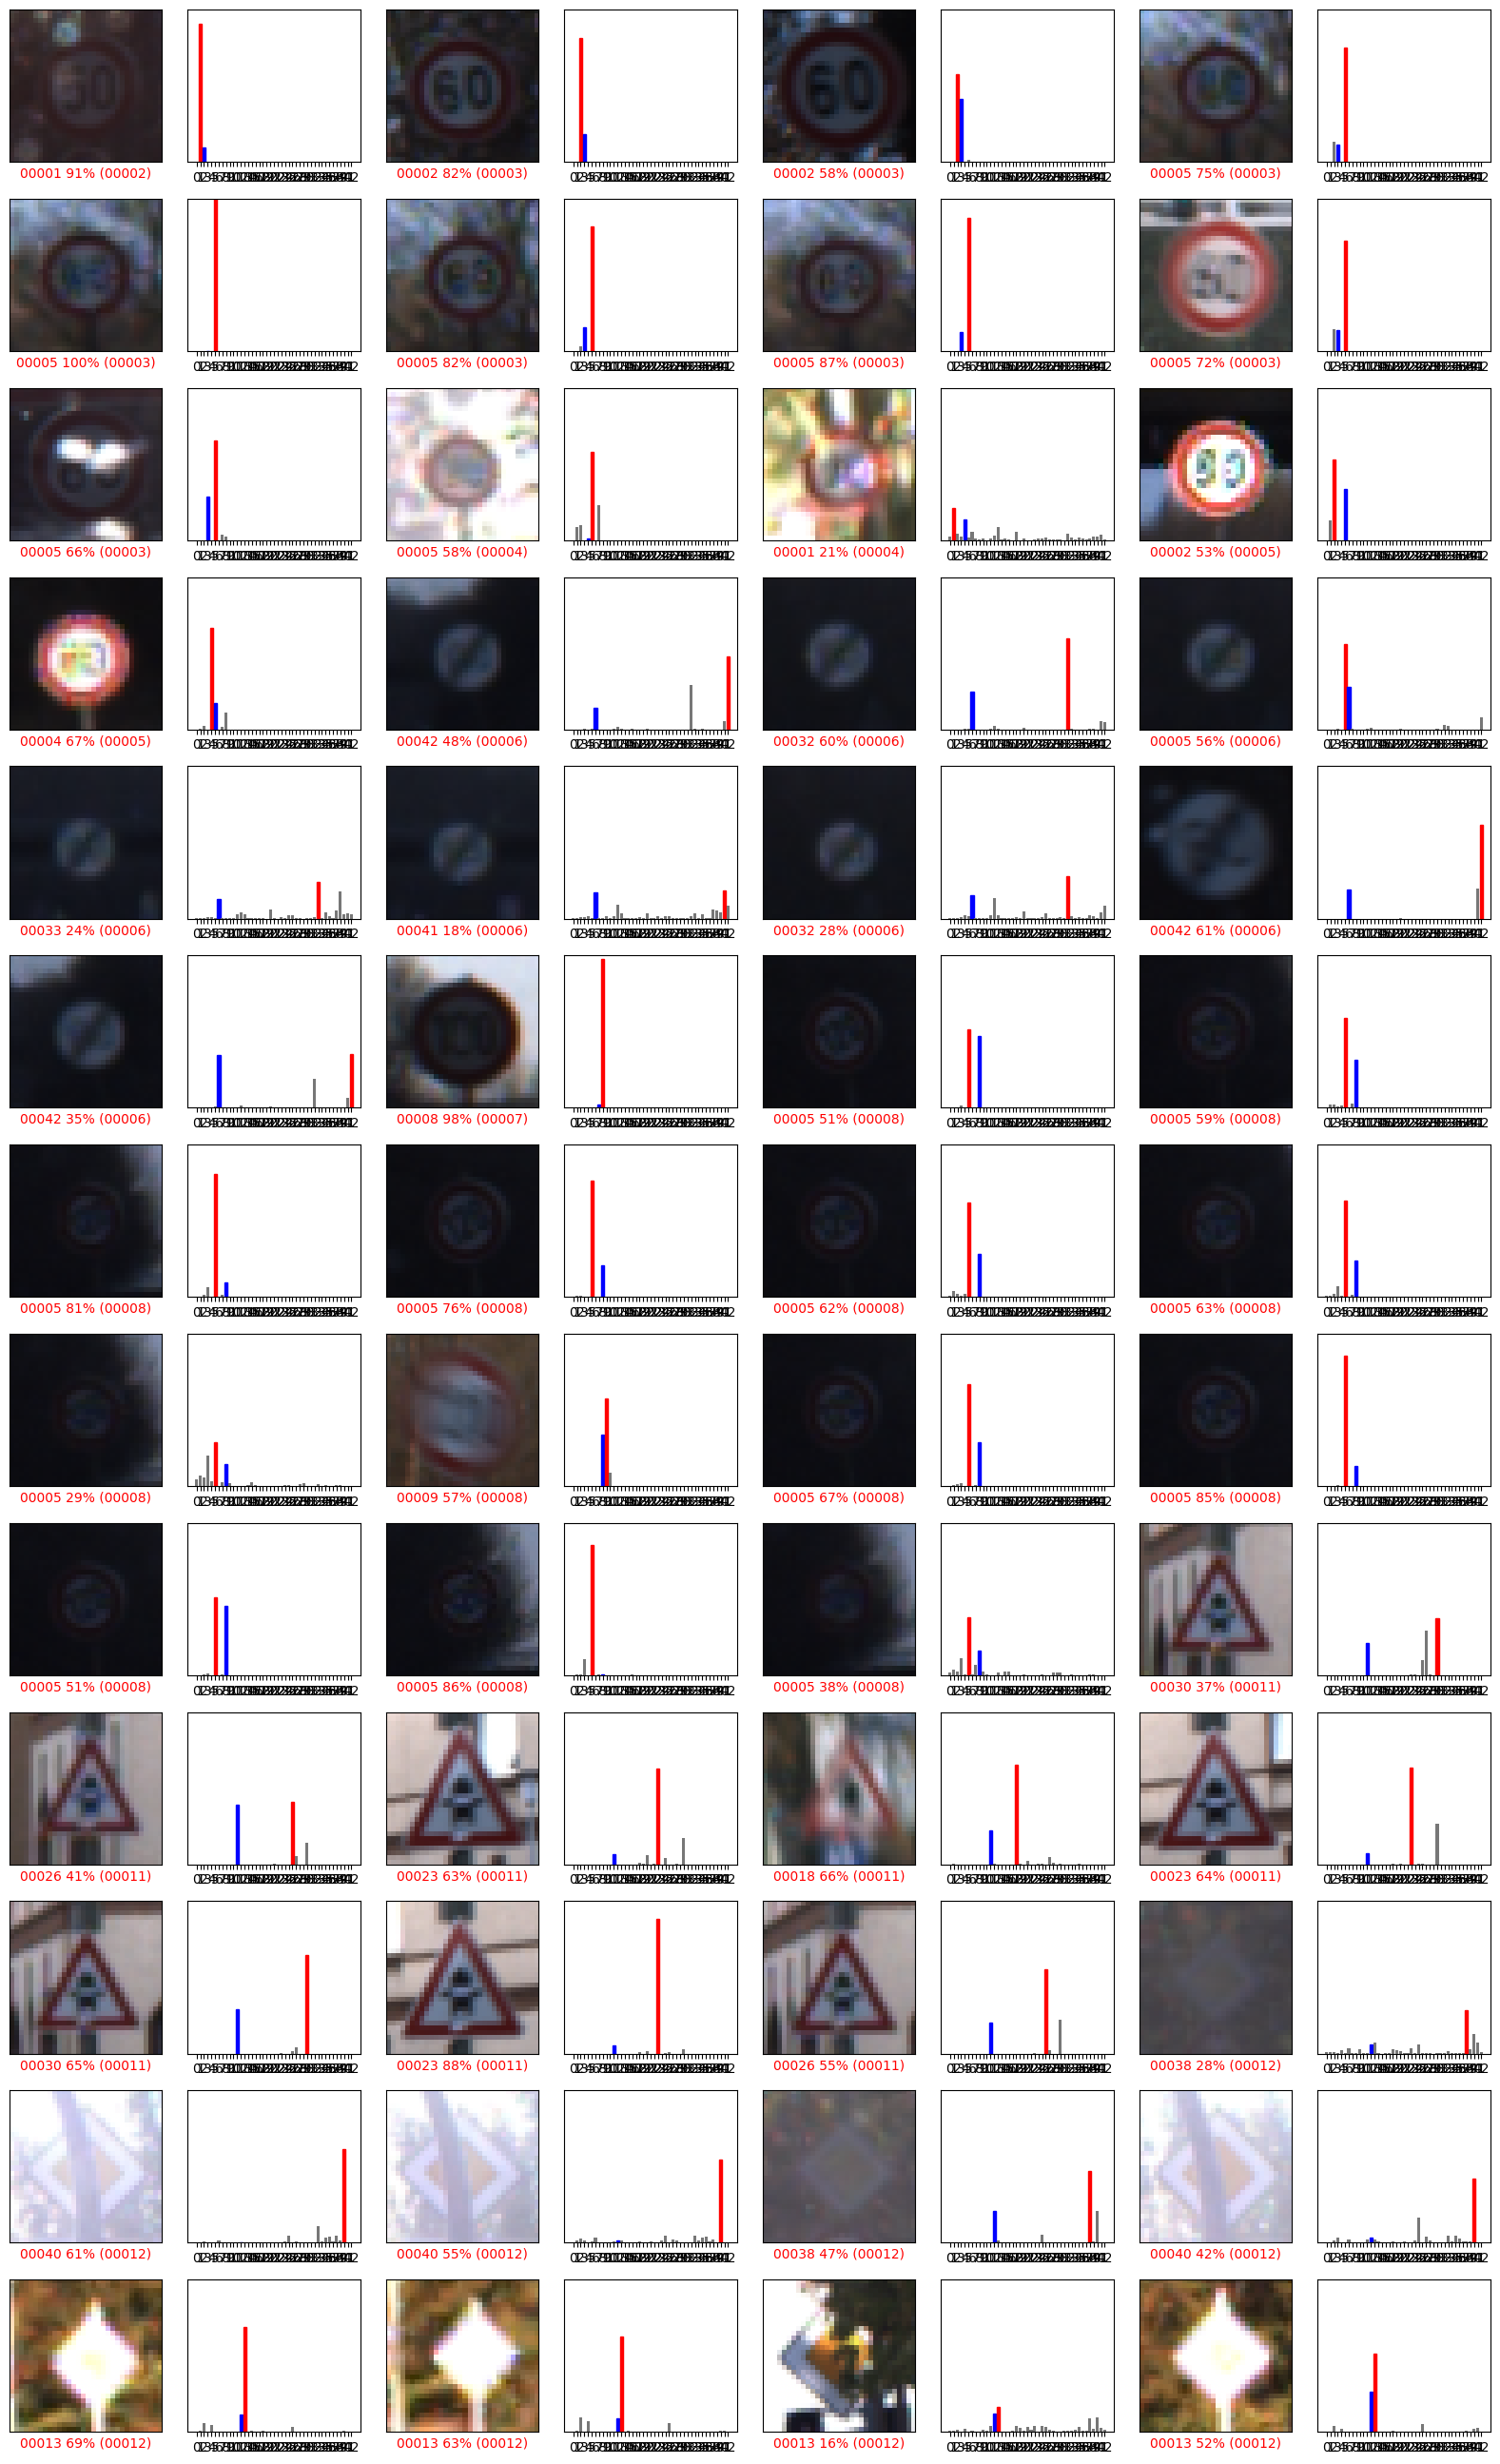
\includegraphics[width=0.8\linewidth]{images/static_colorjitter_bad_predictions.png}
    \caption{Static ColorJitter misclassified samples.}
    \label{fig:static_colorjitter_bad_predictions}
\end{figure}

\subsubsection{RandomAffine}

\begin{figure}[h]
    \centering
    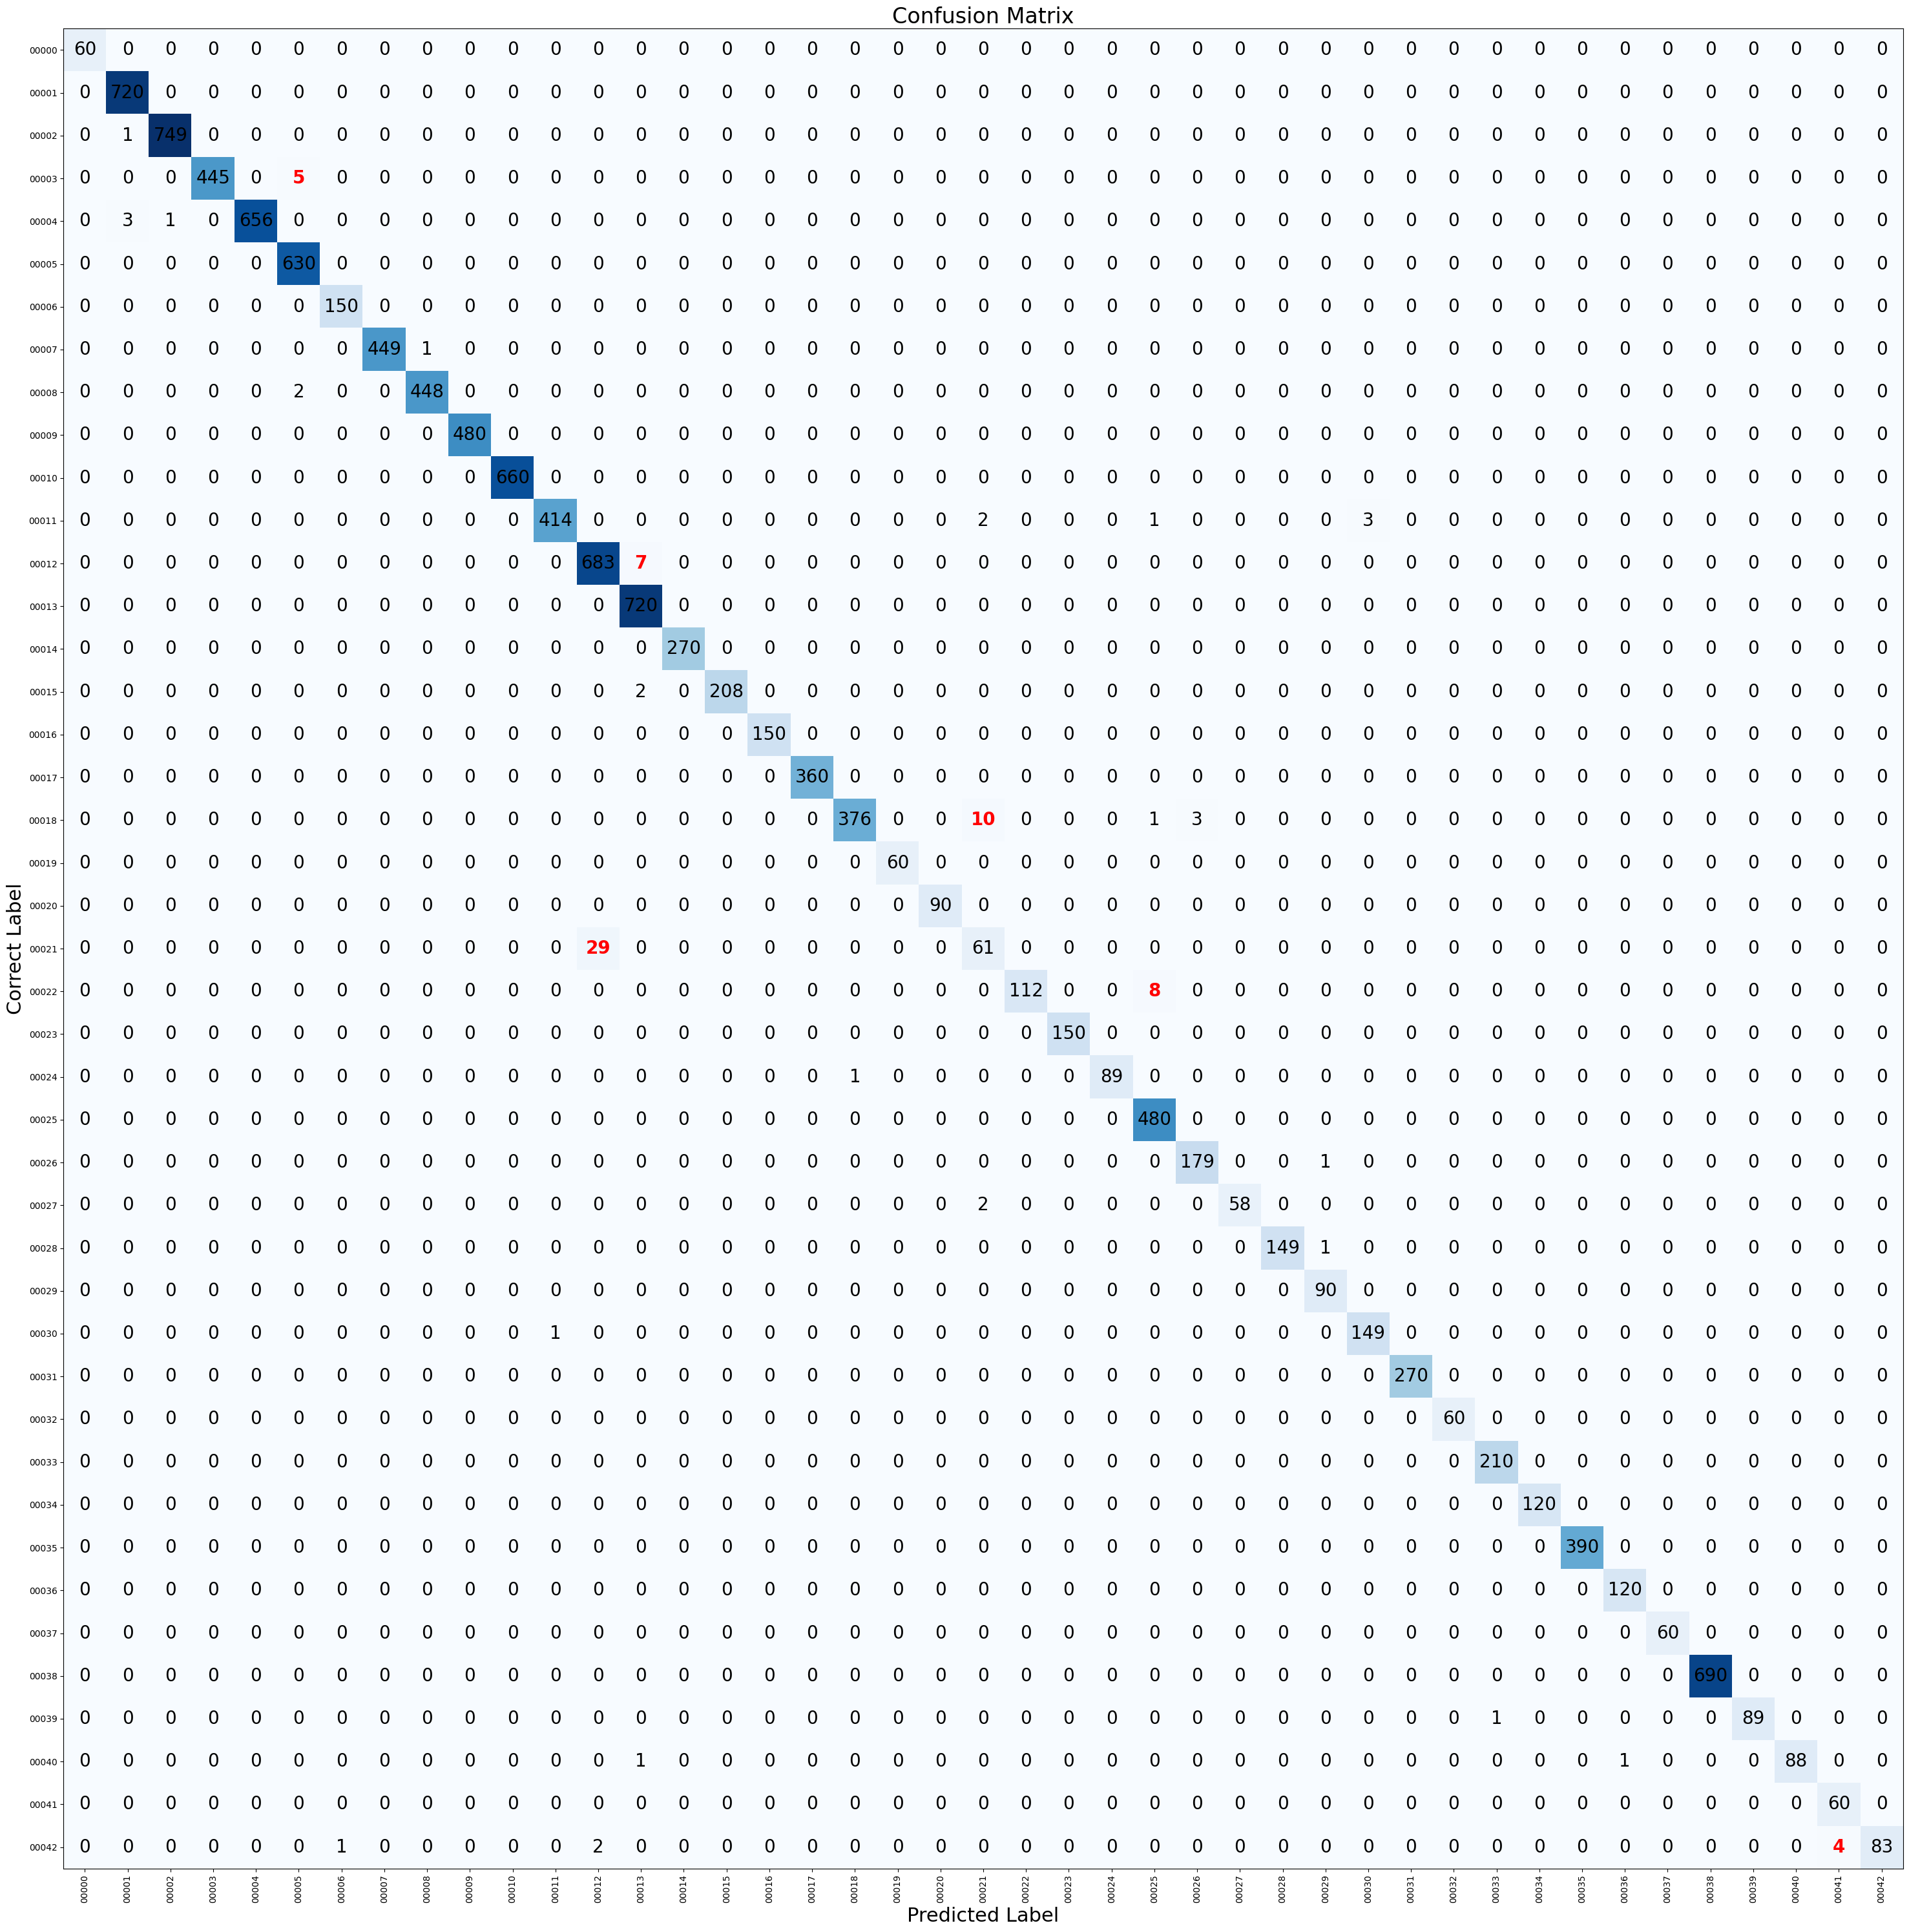
\includegraphics[width=0.8\linewidth]{images/static_affine_confusion_matrix.png}
    \caption{Static RandomAffine confusion matrix.}
    \label{fig:static_affine_confusion_matrix}
\end{figure}

\begin{figure}[h]
    \centering
    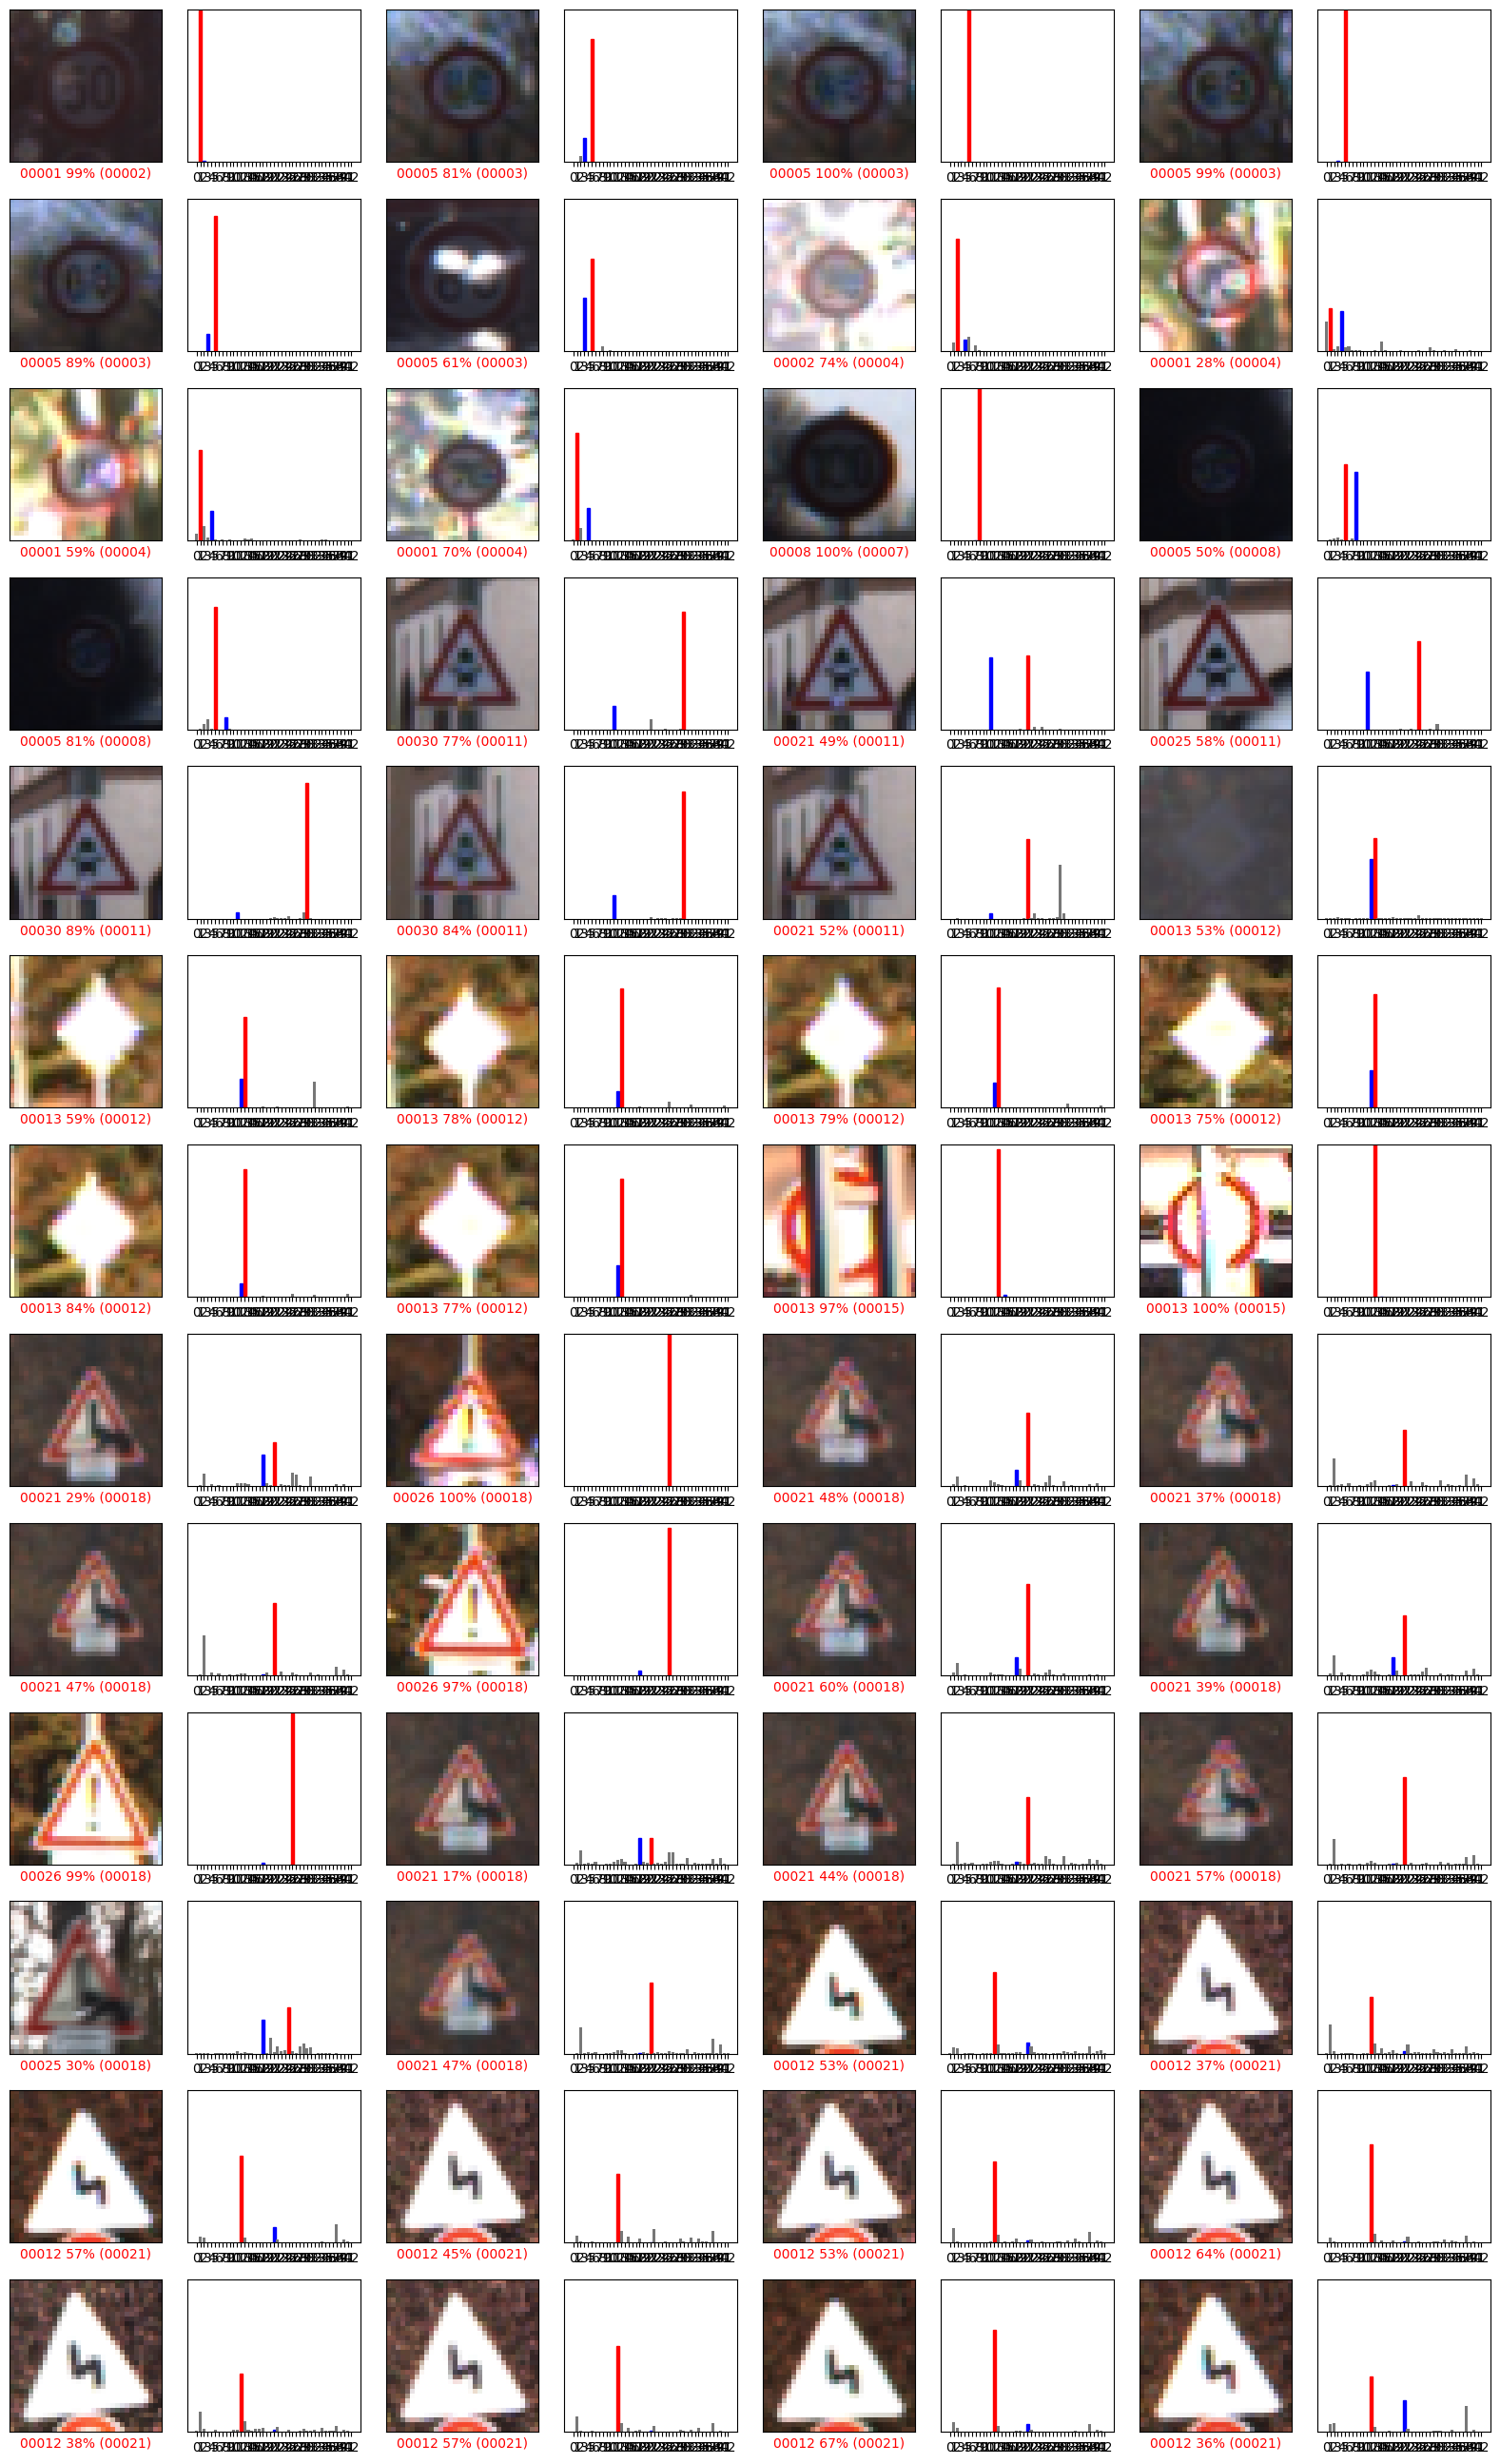
\includegraphics[width=0.8\linewidth]{images/static_affine_bad_predictions.png}
    \caption{Static RandomAffine misclassified samples.}
    \label{fig:static_affine_bad_predictions}
\end{figure}

\subsubsection{Gaussian Blur}

\begin{figure}[h]
    \centering
    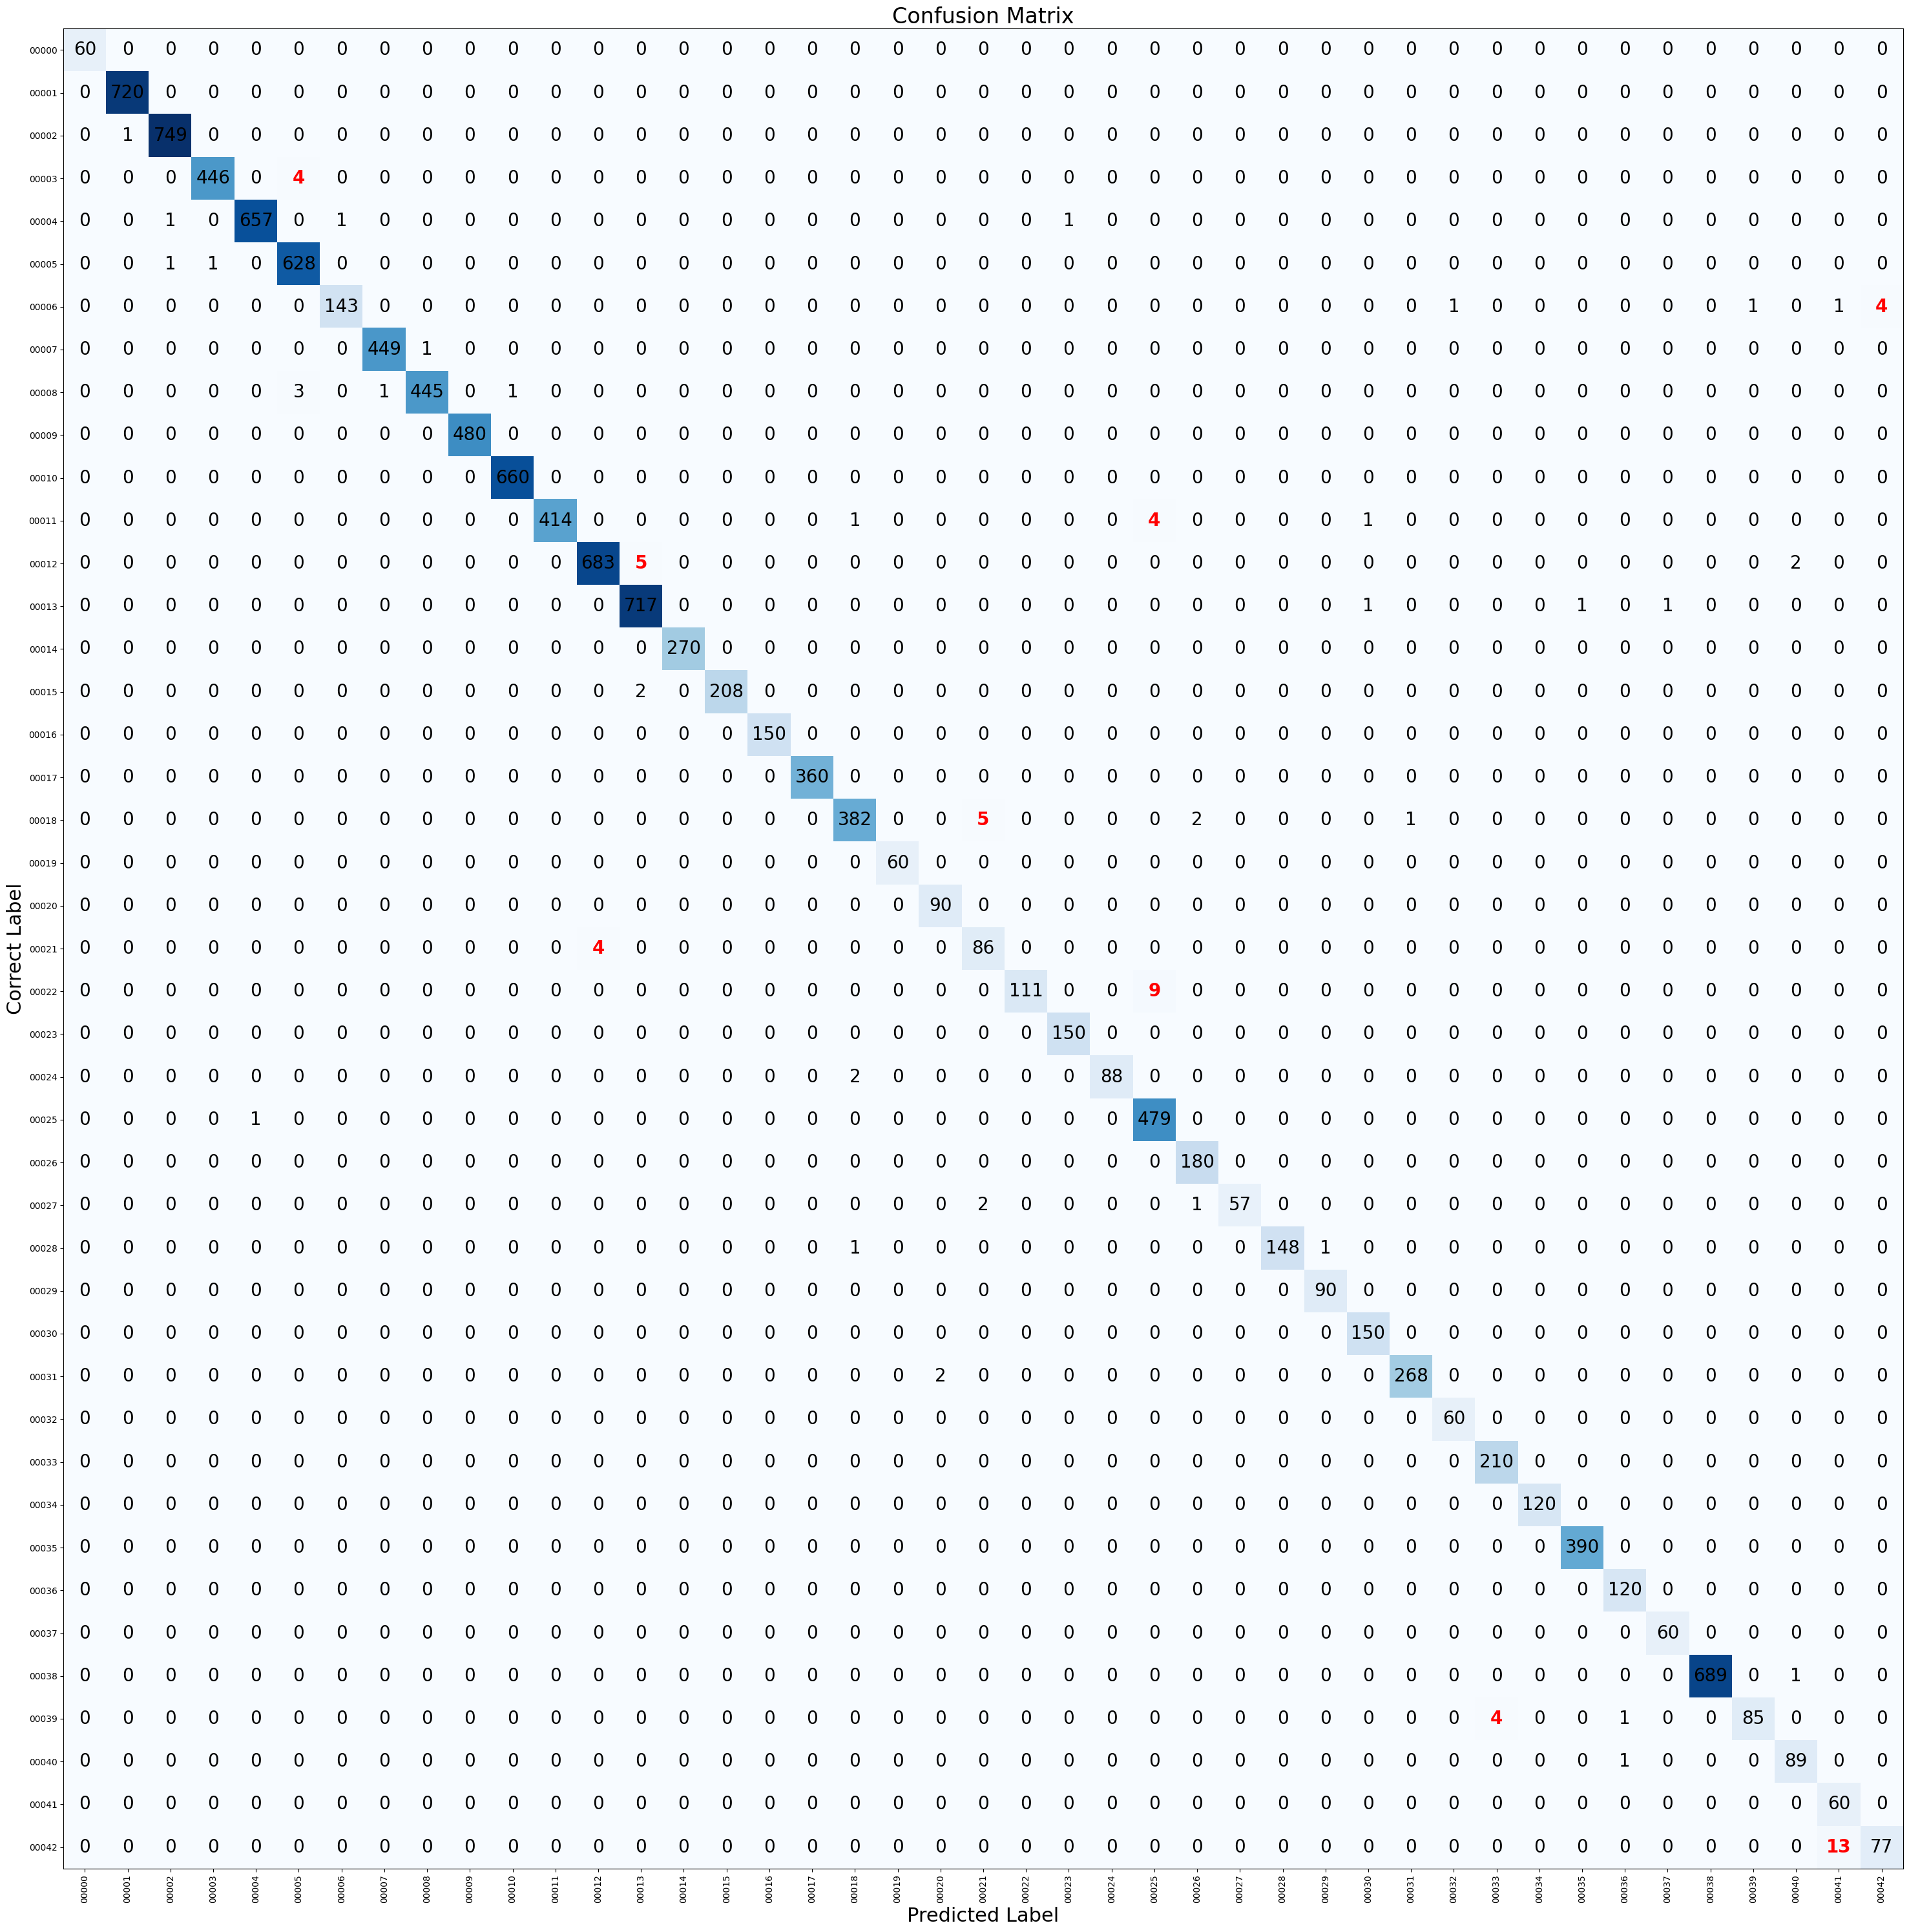
\includegraphics[width=0.8\linewidth]{images/static_blur_confusion_matrix.png}
    \caption{Static Gaussian Blur confusion matrix.}
    \label{fig:static_blur_confusion_matrix}
\end{figure}

\begin{figure}[h]
    \centering
    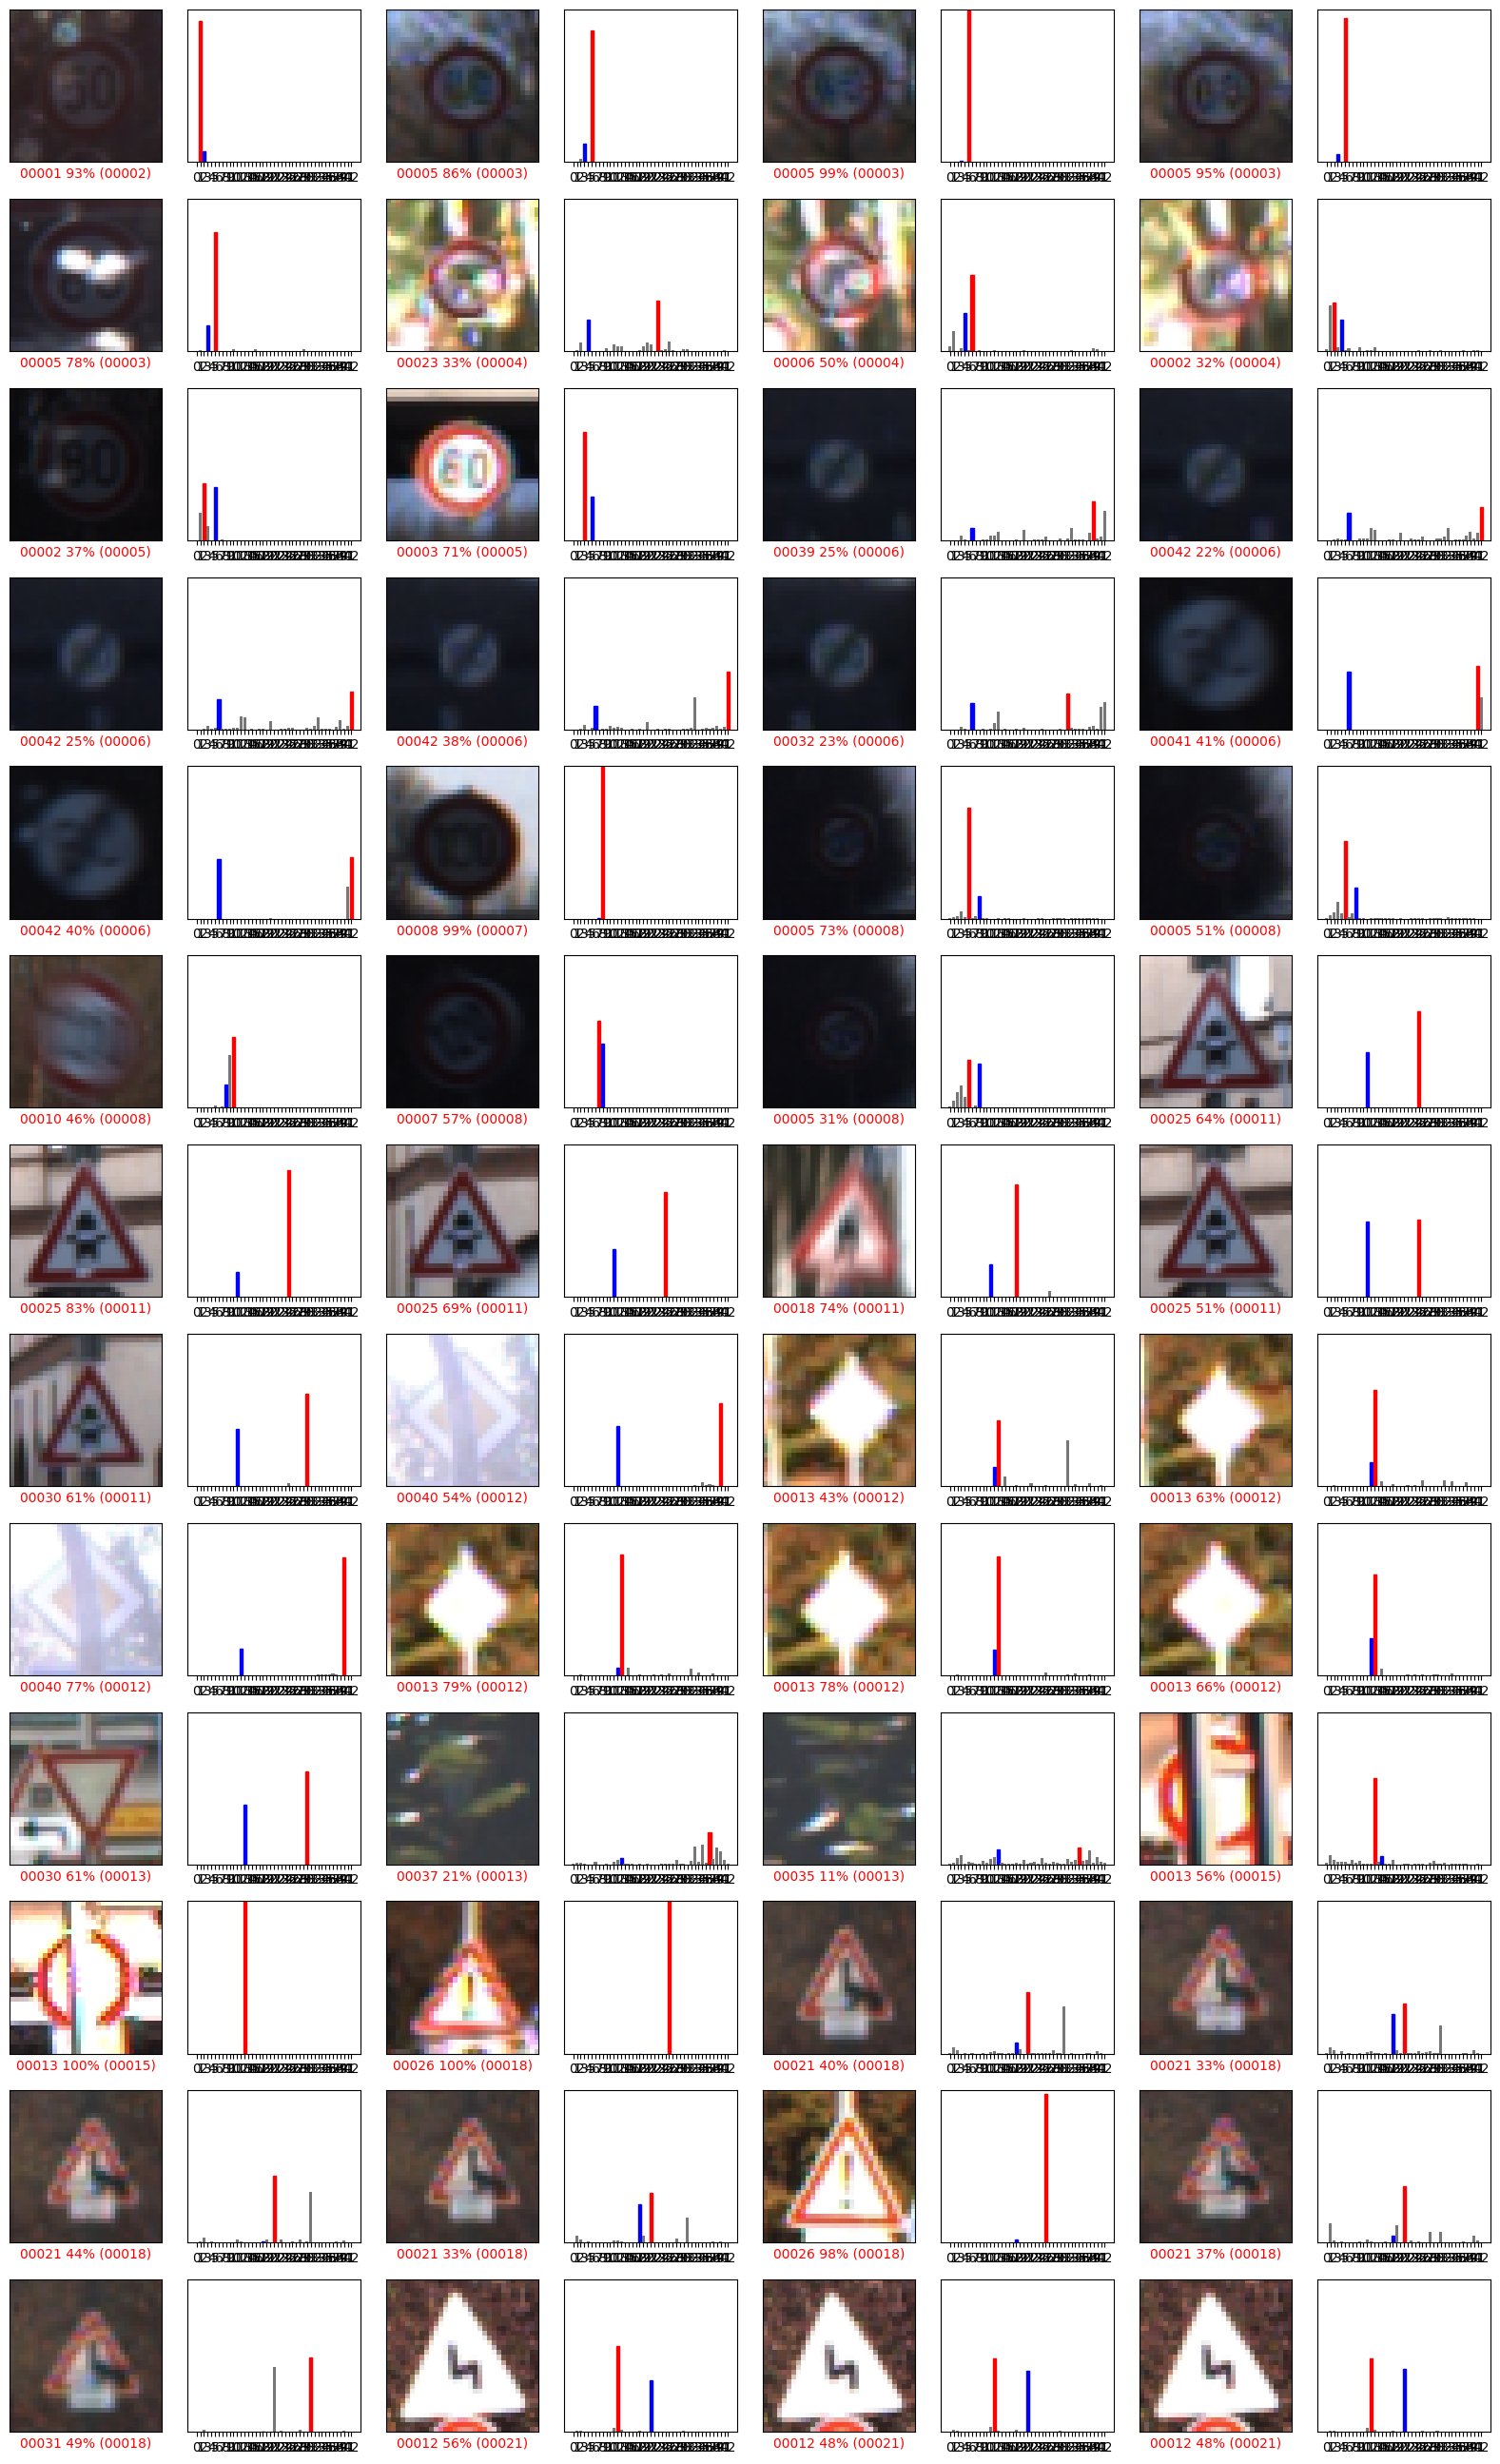
\includegraphics[width=0.8\linewidth]{images/static_blur_bad_predictions.png}
    \caption{Static Gaussian Blur misclassified samples.}
    \label{fig:static_blur_bad_predictions}
\end{figure}

\subsubsection{Random Erasing}

\begin{figure}[h]
    \centering
    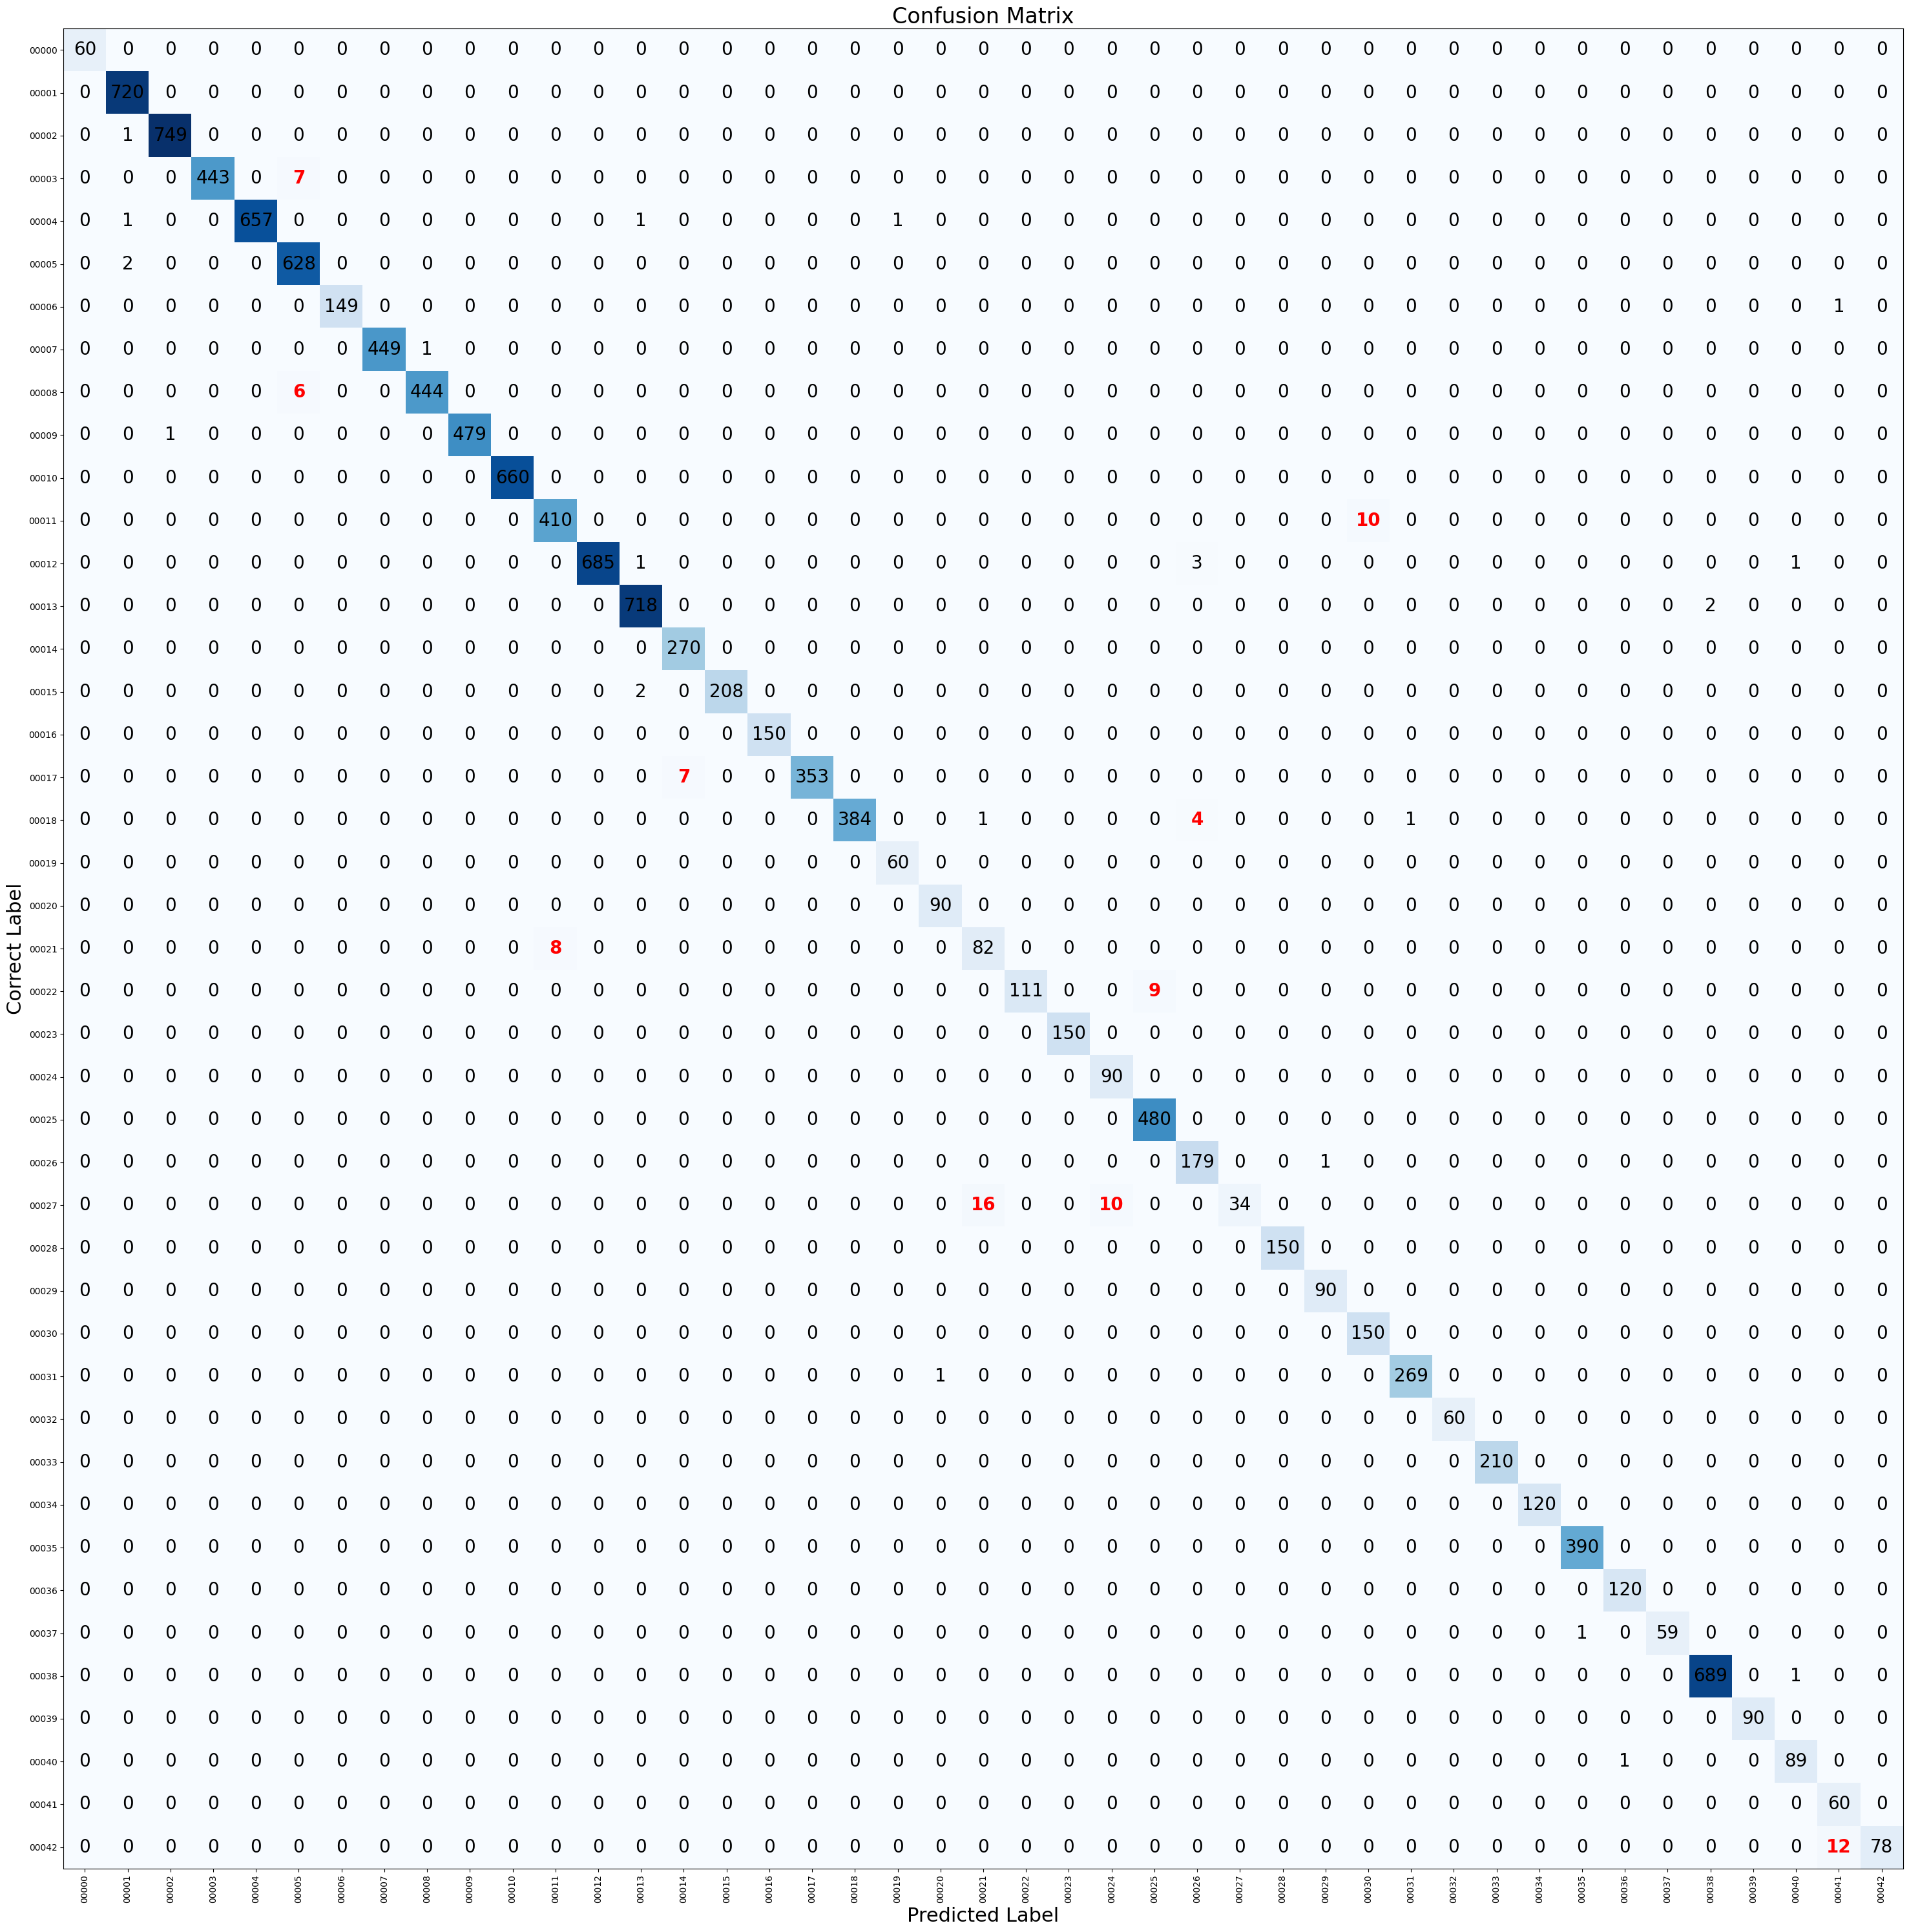
\includegraphics[width=0.8\linewidth]{images/static_erasing_confusion_matrix.png}
    \caption{Static Random Erasing confusion matrix.}
    \label{fig:static_erasing_confusion_matrix}
\end{figure}

\begin{figure}[h]
    \centering
    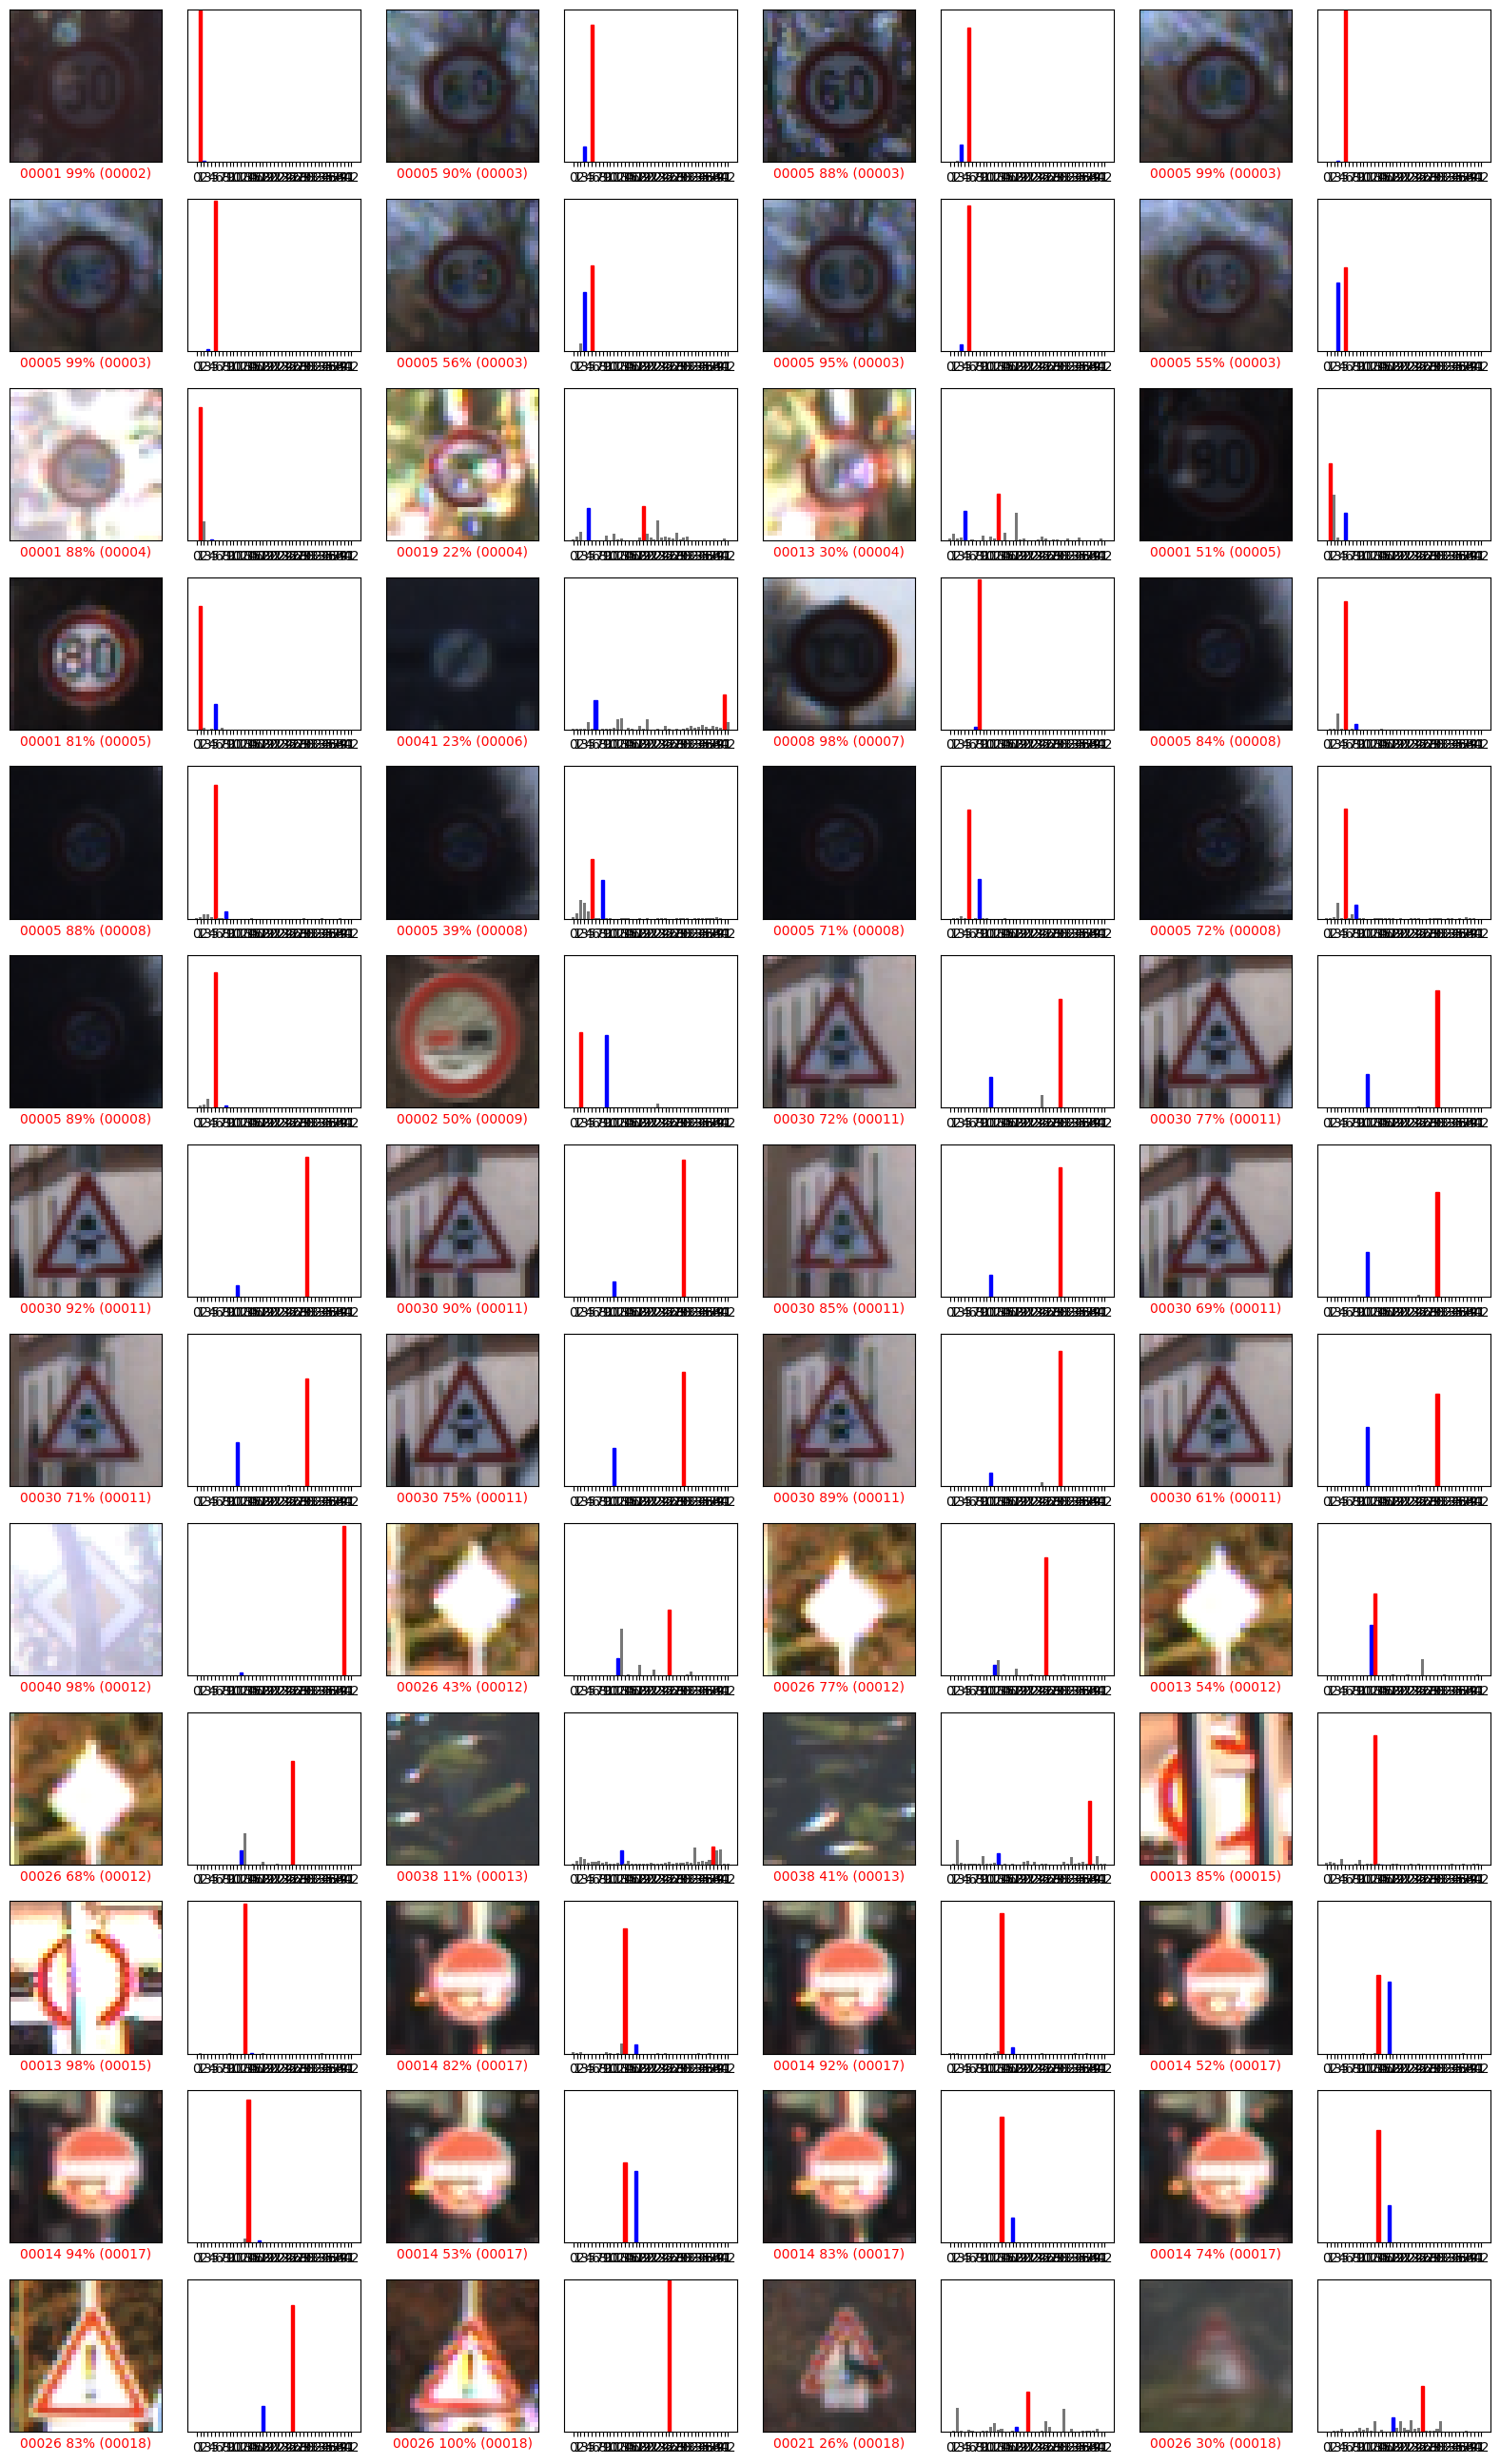
\includegraphics[width=0.8\linewidth]{images/static_erasing_bad_predictions.png}
    \caption{Static Random Erasing misclassified samples.}
    \label{fig:static_erasing_bad_predictions}
\end{figure}

\subsubsection{Combined Static}

\begin{figure}[h]
    \centering
    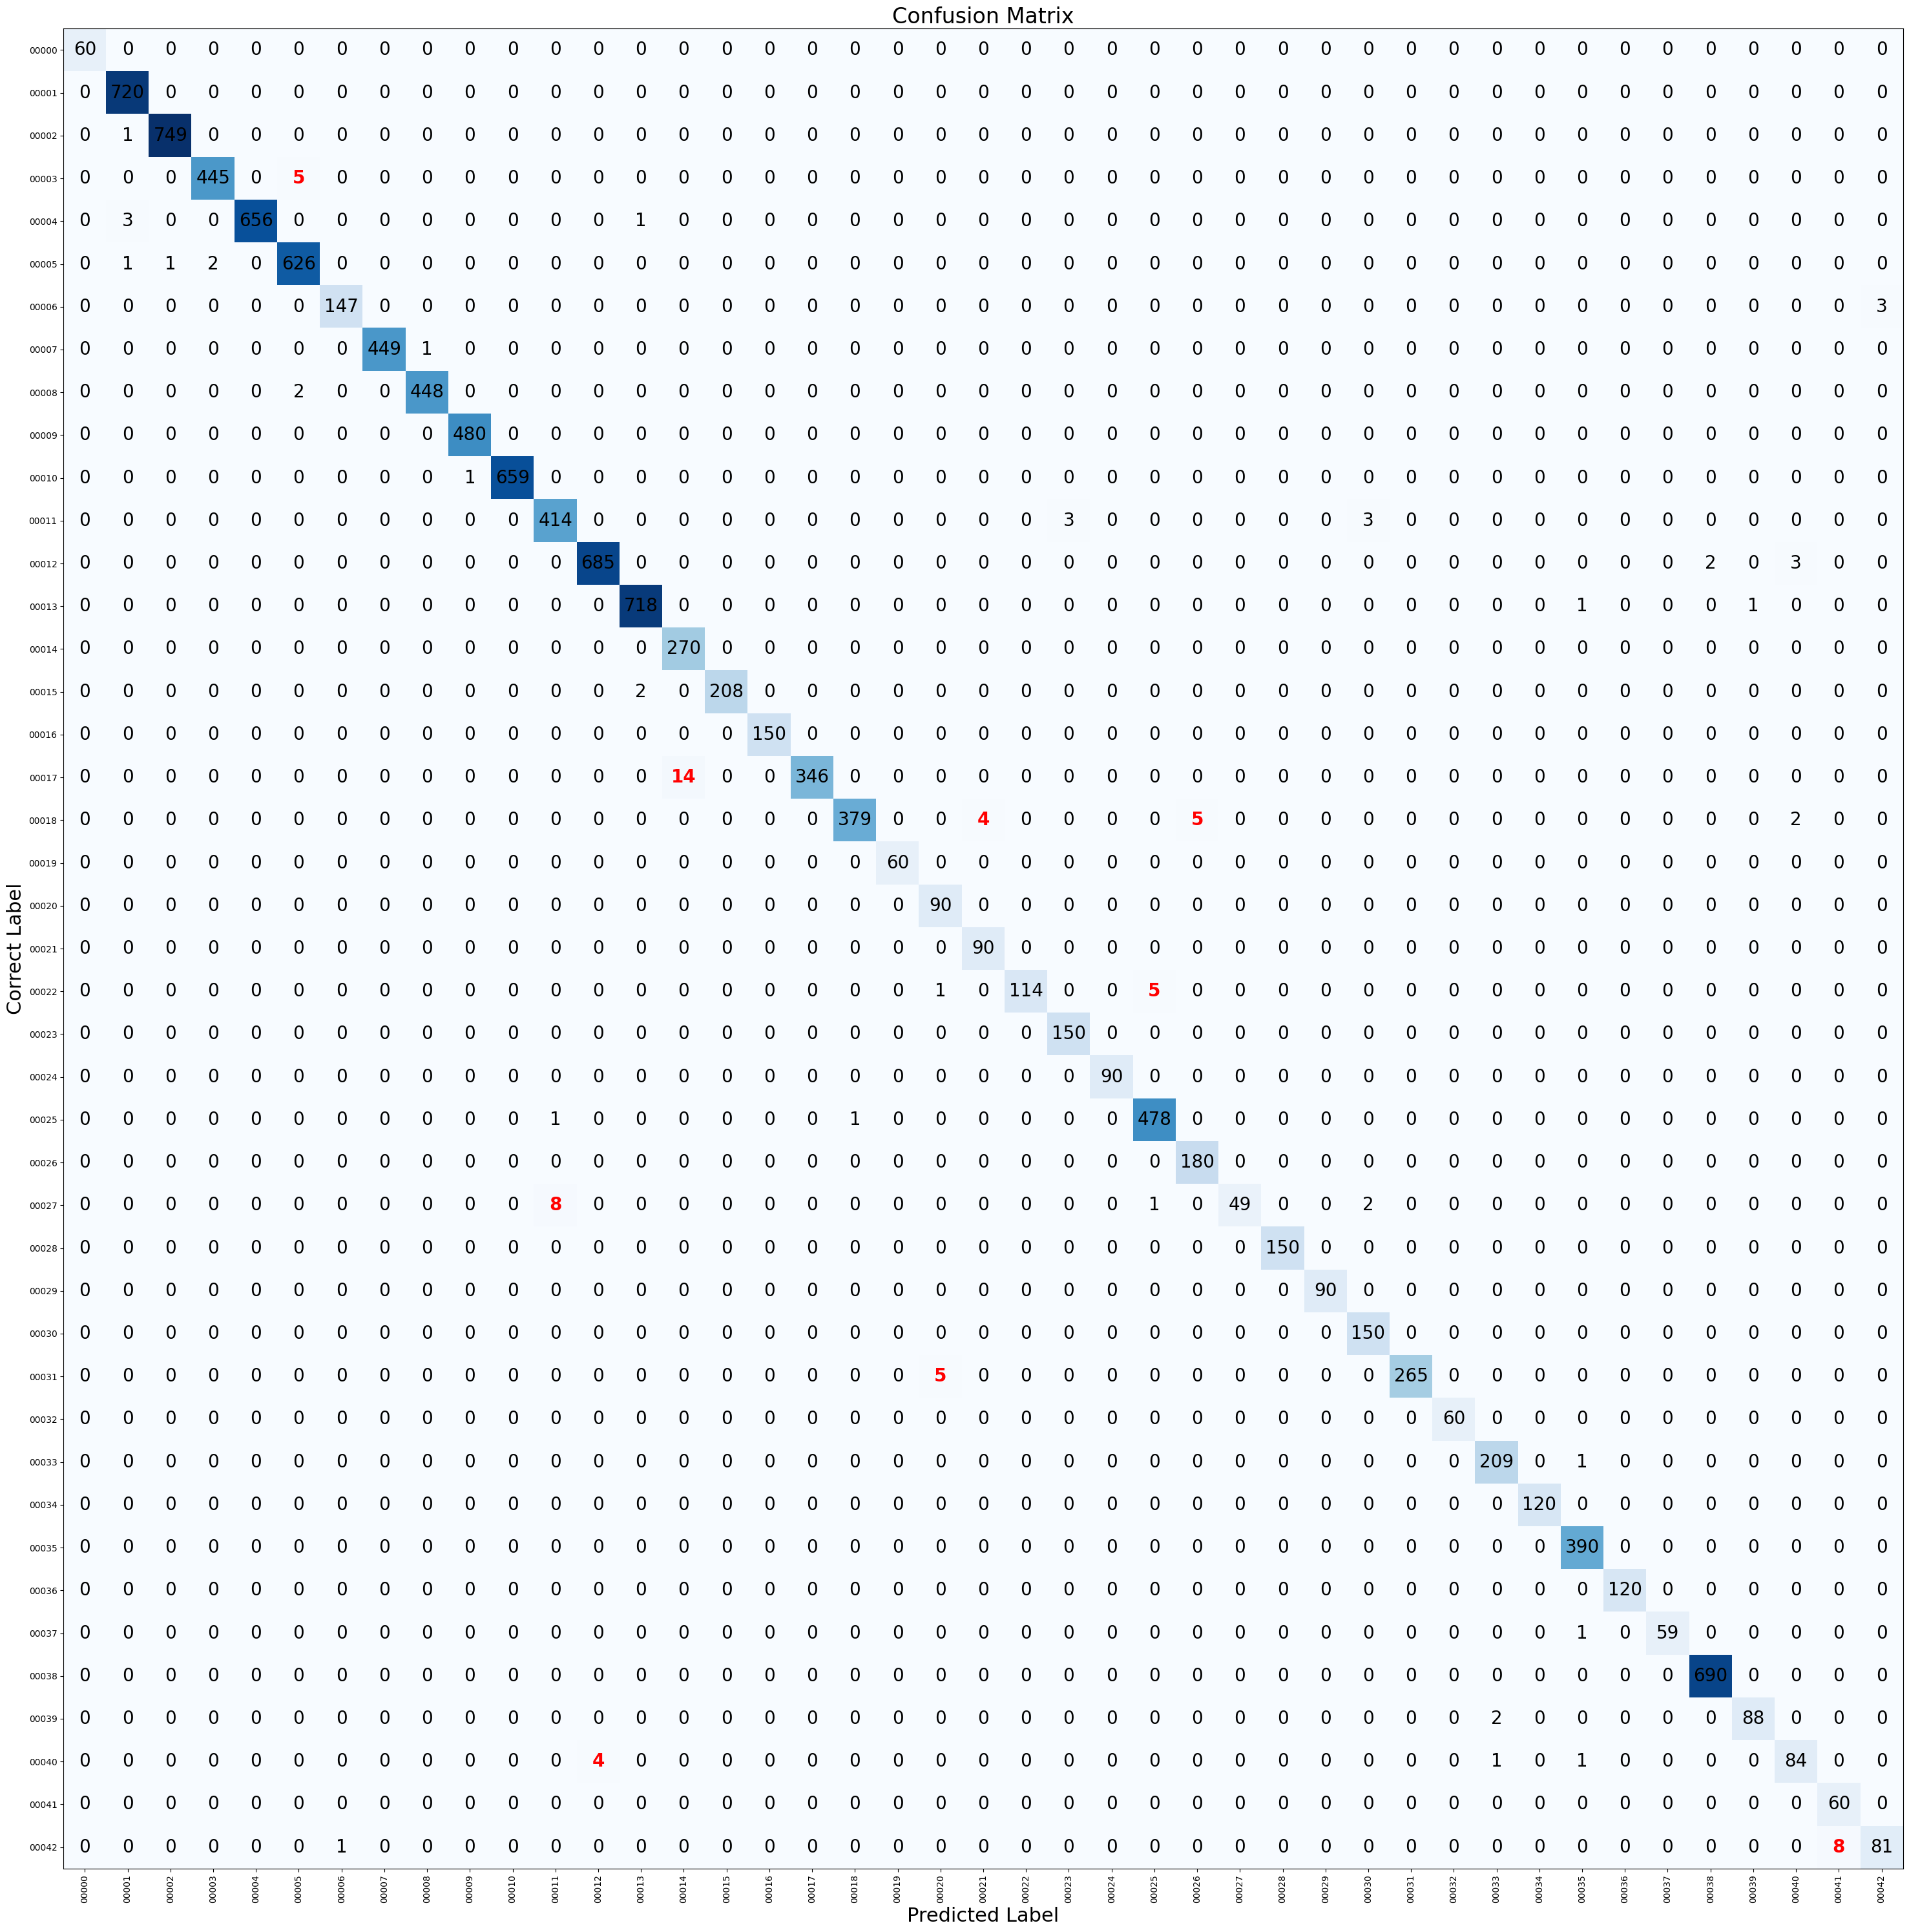
\includegraphics[width=0.8\linewidth]{images/static_combined_confusion_matrix.png}
    \caption{Combined static augmentation confusion matrix.}
    \label{fig:static_combined_confusion_matrix}
\end{figure}

\begin{figure}[h]
    \centering
    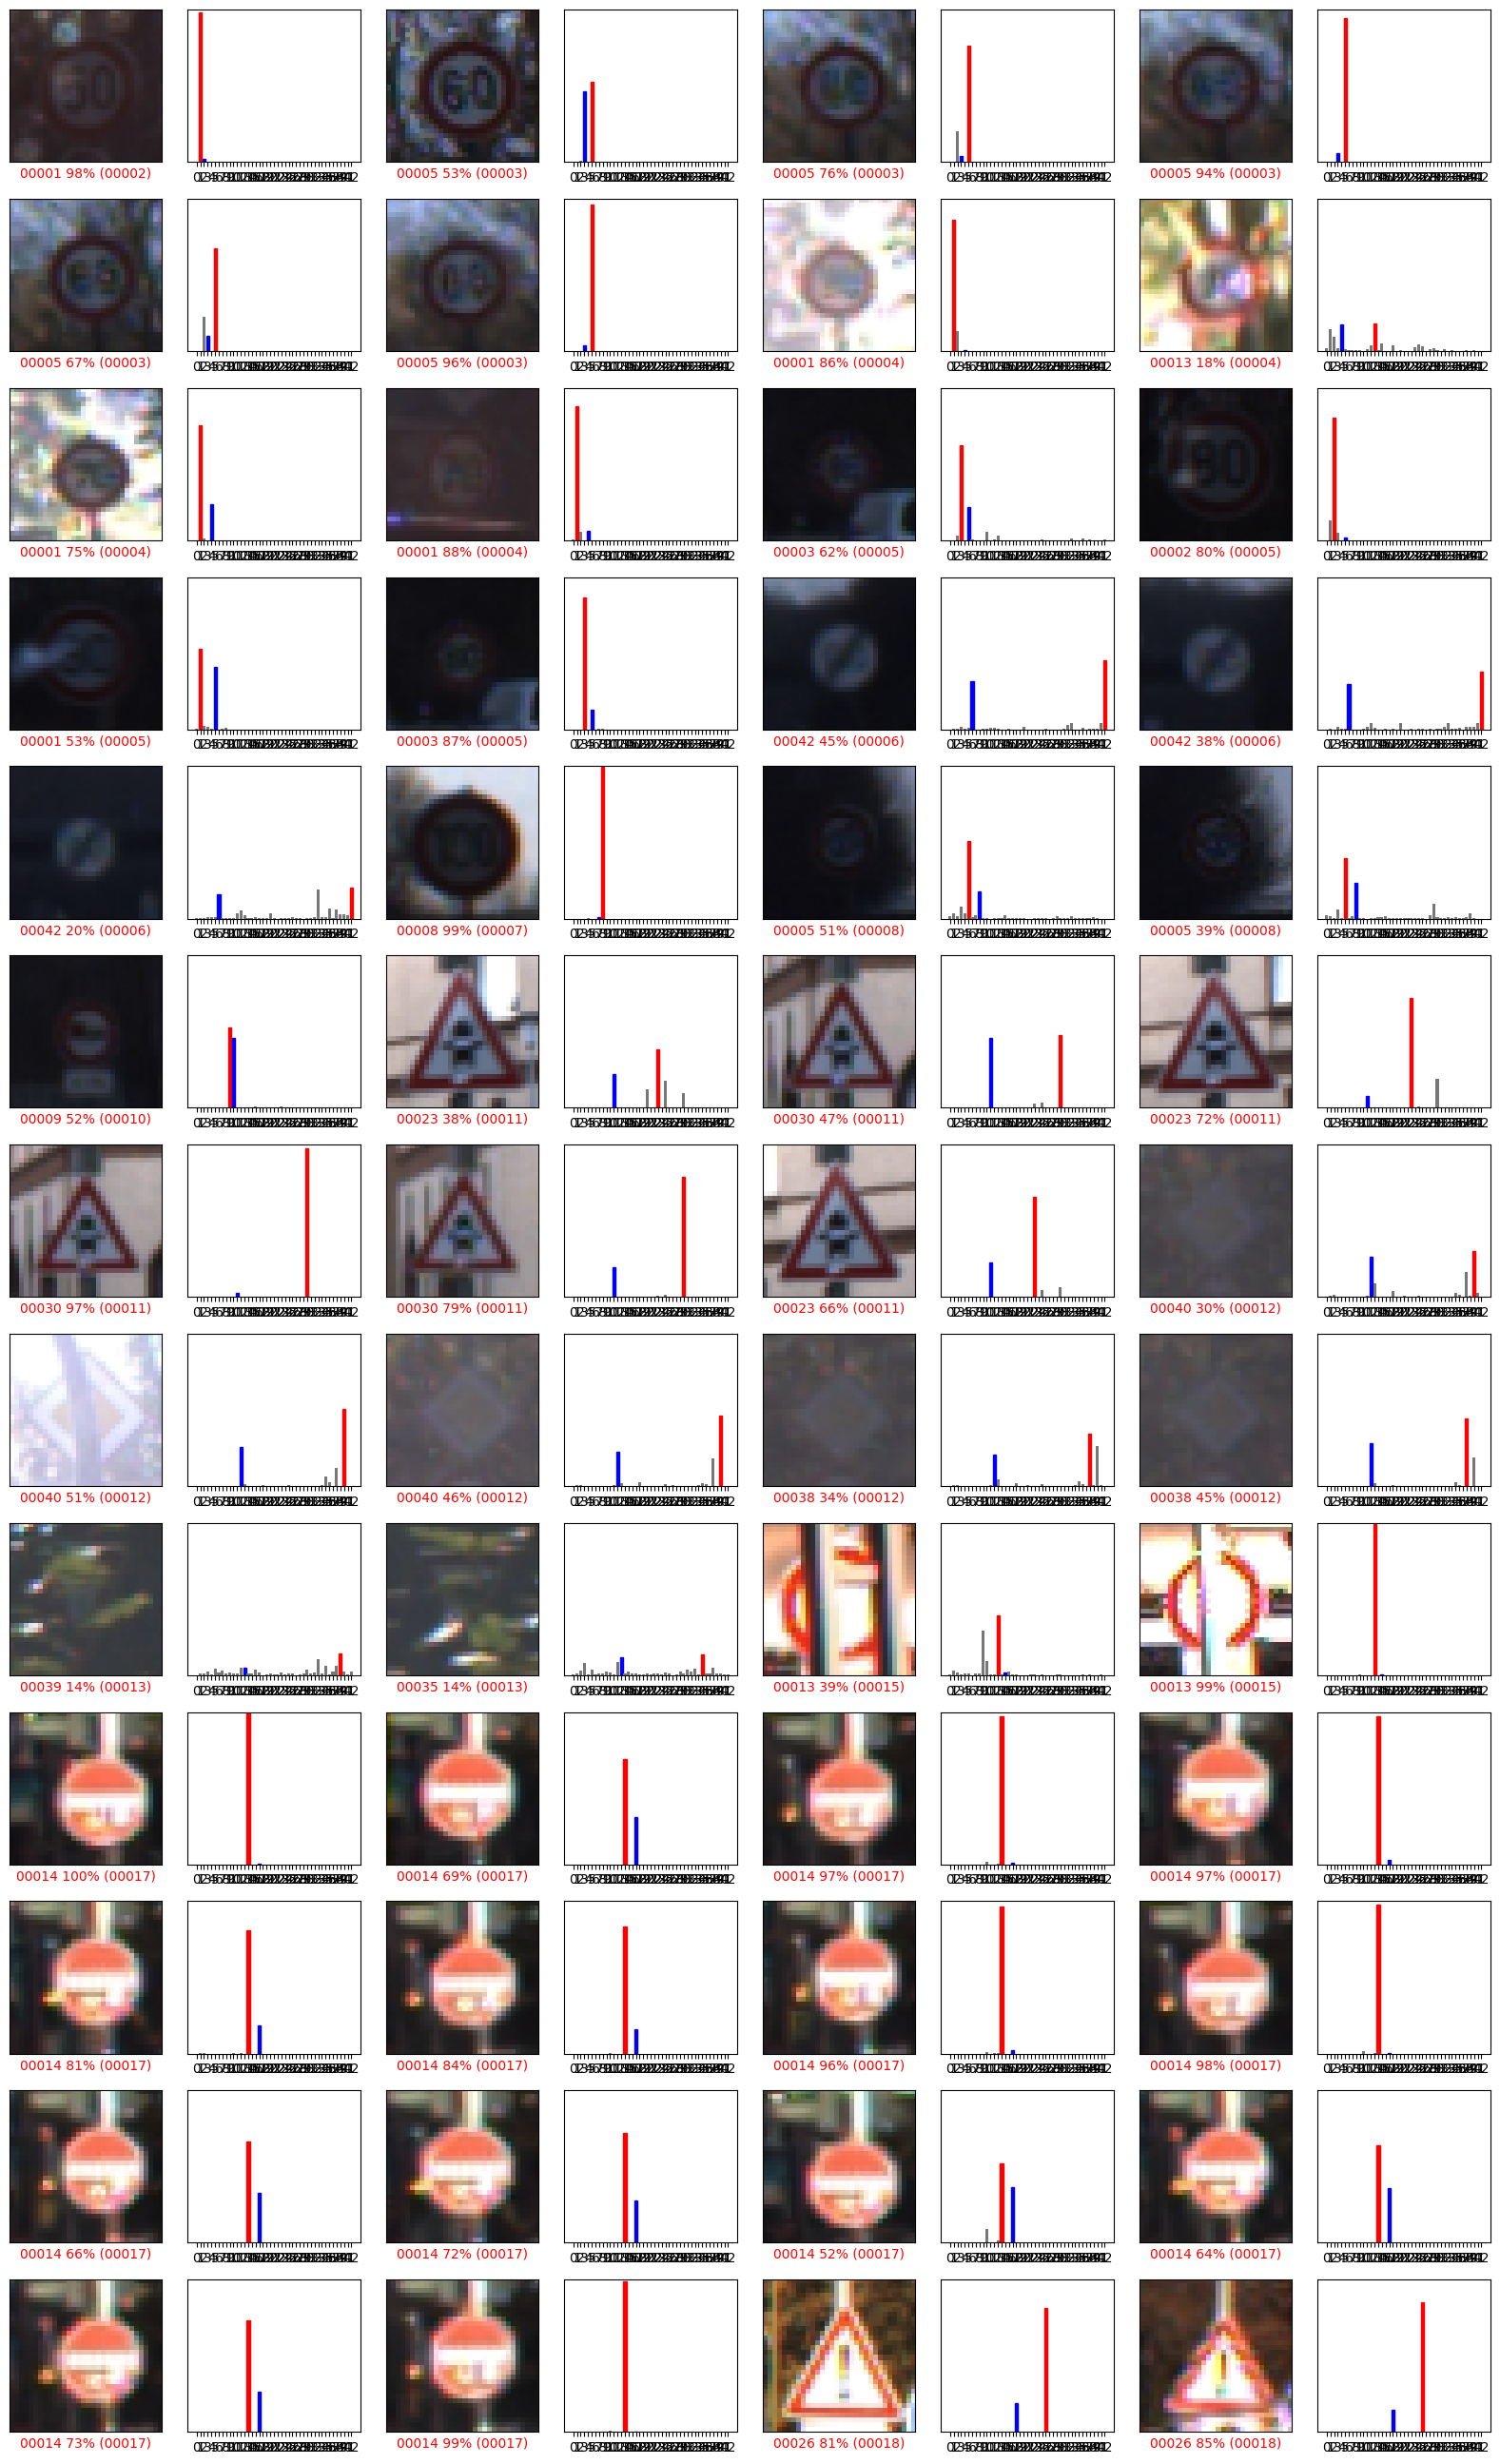
\includegraphics[width=0.8\linewidth]{images/static_combined_bad_predictions.png}
    \caption{Combined static augmentation misclassified samples.}
    \label{fig:static_combined_bad_predictions}
\end{figure}






\end{document}
